\documentclass[11pt]{article}
\usepackage[T1]{fontenc}
\usepackage{lmodern}
\usepackage[margin=1.05in]{geometry}
\usepackage{amsmath,amssymb,amsthm,mathtools}
\usepackage{mathrsfs}
\usepackage{microtype}
\usepackage{needspace}
\usepackage{graphicx}
\usepackage{float}
\usepackage{tikz}
\usepackage{tikz-cd}
\usetikzlibrary{arrows.meta,positioning,calc,fit}
\usepackage[colorlinks=true,linkcolor=blue!45!black,citecolor=blue!45!black,urlcolor=blue!45!black]{hyperref}
\hypersetup{pdftitle={Counterexamples to the Hahn-Wilson conjecture at height two},pdfauthor={OpenAI}}
\DeclareMathOperator{\Thick}{Thick}
\DeclareMathOperator{\Spec}{Spec}
\DeclareMathOperator{\Hom}{Hom}
\DeclareMathOperator{\Ext}{Ext}
\DeclareMathOperator{\Tor}{Tor}
\DeclareMathOperator{\gr}{gr}
\DeclareMathOperator{\cofib}{cofib}
\DeclareMathOperator{\fib}{fib}
\DeclareMathOperator{\hocolim}{hocolim}
\DeclareMathOperator{\holim}{holim}
\DeclareMathOperator{\coker}{coker}
\DeclareMathOperator{\im}{im}
\DeclareMathOperator{\id}{id}
\DeclareMathOperator{\Perf}{Perf}
\DeclareMathOperator{\Mod}{Mod}
\DeclareMathOperator{\CT}{CT}
\newcommand{\Sp}{\mathrm{Sp}}
\newcommand{\BP}{\mathrm{BP}}
\newcommand{\Z}{\mathbb Z}
\newcommand{\F}{\mathbb F}
\newcommand{\Q}{\mathbb Q}
\newcommand{\Gm}{\mathbb G_m}
\newtheorem{theorem}{Theorem}[section]
\newtheorem{lemma}[theorem]{Lemma}
\newtheorem{proposition}[theorem]{Proposition}
\newtheorem{corollary}[theorem]{Corollary}
\theoremstyle{definition}
\newtheorem{definition}[theorem]{Definition}
\newtheorem{notation}[theorem]{Notation}
\theoremstyle{remark}
\newtheorem{remark}[theorem]{Remark}
\newtheorem{example}[theorem]{Example}
\numberwithin{equation}{section}
\setcounter{tocdepth}{2}
\title{Counterexamples to the Hahn--Wilson conjecture at height two}
\author{OpenAI}
\date{September 26, 2026}

\begin{document}
\maketitle
\begin{abstract}
We disprove the Hahn--Wilson conjecture at height two. For every sufficiently
large prime $p$, we construct a connective $p$-complete spectrum $X$ of exact
fp-type two outside the ordinary thick subcategory generated by the specified
standard form of $\BP\langle2\rangle_p^\wedge$. The same spectrum satisfies
both localization comparisons
$L_2^fX\simeq L_2X$ and $L_{T(2)}X\simeq L_{K(2)}X$.
\end{abstract}

\section{Introduction}\label{sec:introduction}

Which infinite spectra can be built from truncated Brown--Peterson
spectra using finitely many cofiber sequences and retracts?
The Hahn--Wilson conjecture proposes a cohomological answer: finite
presentation over the Steenrod algebra, together with a chromatic
height bound, should characterize precisely these finite constructions.
We construct counterexamples at height two. Their chromatic
localizations retain strong finiteness properties; the obstruction
lies in how the local pieces are joined.

\subsection{The question and the theorem}

Fix a prime $p$. Write $K(j)$ for Morava $K$-theory, with $K(0)=H\Q$.
A nonzero finite $p$-local spectrum has \emph{type} $j$ if $j$ is the
least index for which its $K(j)$-homology is nonzero. The thick
subcategory theorem classifies thick subcategories of finite
$p$-local spectra by type
\cite{HS1998}.

A bounded-below $p$-complete spectrum $X$ is \emph{fp} if
$H^*(X;\F_p)$ is finitely presented over the mod-$p$ Steenrod algebra.
Mahowald and Rezk prove that this is equivalent to requiring
$\pi_*(V\wedge X)$ to be finite in total for some nonzero finite
$p$-local spectrum $V$ \cite[Proposition~3.2]{MR1999}.
Here \emph{finite in total} means finitely many nonzero homotopy
groups, each a finite group. For an fp-spectrum, fp-type at most $n$
means that this test holds for a finite spectrum of type $n+1$,
equivalently for every such spectrum. We include the zero spectrum.
Exact fp-type two means fp-type at most two but not at most one.

For a $p$-complete spectrum $B$, let $\Thick(B)$ be its closure in
$\Sp_p^\wedge$ under equivalences, finite sums, all integer shifts,
cofiber sequences and retracts. These are the permitted operations;
in particular this is ordinary thick closure. The conjecture is
\begin{equation}\label{eq:hw-conjecture}
 \{X:\text{$X$ has fp-type at most $n$}\}
 =\Thick(\BP\langle n\rangle_p^\wedge).
\end{equation}
Its written formulation appears in Lee--Pstr\k{a}gowski
\cite[Conjecture~1.1 and Note~1]{LP2026}, who report learning it from Dylan Wilson
in 2021. A standard completed truncated Brown--Peterson spectrum has
coefficients $\Z_p[v_1,\ldots,v_n]$, where $|v_i|=2(p^i-1)$.

Let $L_n=L_{E(n)}$ denote Johnson--Wilson localization and $L_n^f$
finite localization away from finite spectra of type greater than $n$.
For $n>0$, let $T(n)$ be a telescope of a periodic self-map of a finite
type-$n$ spectrum.

\begin{theorem}\label{thm:main}
For every sufficiently large prime $p$, there is a connective
$p$-complete spectrum $X$ of exact fp-type two such that, for a
standard form of $\BP\langle2\rangle_p^\wedge$,
\[
 X\notin\Thick(\BP\langle2\rangle_p^\wedge).
\]
The same spectrum satisfies
\[
 L_2^fX\simeq L_2X,
 \qquad L_{T(2)}X\simeq L_{K(2)}X.
\]
\end{theorem}

The theorem refutes the universally quantified conjecture
\eqref{eq:hw-conjecture}; its prime range is sufficiently large primes.
We use a specific regular $\BP$-module quotient throughout the proof.
At these odd primes the underlying spectrum is independent of the
standard quotient generators \cite[Corollary~1.9]{Lee2026}.
This uniqueness uses the work of Angeltveit--Lind, with its corrected
argument and the additional $p$-local result supplied by Lee
\cite{AL2017,Lee2026}.

\subsection{Global finiteness and the local classification}

Mahowald--Rezk's duality theory makes fp-spectra a natural class of
infinite spectra with controlled chromatic behavior
\cite[Theorem~8.11]{MR1999}. Hahn--Wilson's redshift theorem gives
further examples: for the multiplicative forms in their theorem,
$K(\BP\langle n\rangle_p^\wedge)_p^\wedge$ has fp-type $n+1$
\cite[Theorem~B]{HW2022}. The cases of fp-type at most $-1$ and $0$
are classical, and Lee--Pstr\k{a}gowski prove the global generation
conjecture at height one
\cite[Theorems~1.3 and~5.4]{LP2026}.

Mahowald and Rezk asked whether the comparison
$L_n^fX\to L_nX$ is an equivalence for fp-spectra
\cite[Conjecture~7.3]{MR1999}.
Burklund, Hahn, Levy, and Schlank subsequently disproved the unrestricted
telescope conjecture at every prime and every height at least two
\cite[Theorem~A]{BHLS2023}.
The finiteness distinction remains essential: Lee and Pstr\k{a}gowski
note that the relevant finite-smash homotopy of those counterexamples is
bounded but not finite in total
\cite[Section~1.1, following Conjecture~1.2]{LP2026}.
Thus those counterexamples do not supply the fp counterexample studied here.

There is also a positive classification at every height after Morava
$K$-localization. A $K(n)$-local spectrum $Y$ is \emph{locally fp}
if $\pi_i(F\wedge Y)$ is finite for every integer $i$ and every
finite type-$n$ spectrum $F$. Lee--Pstr\k{a}gowski identify these
objects with $\Thick(E_n)$ in the $K(n)$-local category, equivalently
with $\Thick(L_{K(n)}\BP\langle n\rangle)$
\cite[Theorems~1.7 and~4.3]{LP2026}. Here $E_n$ is Morava
$E$-theory. The height-one local classification has an earlier source
in Hahn--Mitchell's Iwasawa theory \cite[Theorem~8.1]{HM2007}.
The local test requires finiteness in each degree; the global fp-type
test above requires finiteness in total.

Set $X_K=L_{K(2)}X$. Then $X_K\in\Thick(E_2)$, and its cohomology
$E_2^*X_K$ is finitely generated over the ring of operations $E_2^*E_2$.
The natural map from $X_K$ to its double dual, formed using the
$K(2)$-local sphere, is an equivalence. The original
spectrum $X$ has no global finite construction from
$\BP\langle2\rangle_p^\wedge$.
Lee--Pstr\k{a}gowski suggest using a height decomposition and their
local theorem to prove global generation for fp-spectra satisfying
the telescope comparison \cite[Remark~5.1]{LP2026}.
Theorem~\ref{thm:main} shows that this additional hypothesis does not
suffice at height two. The tensor-ideal classification of locally
dualizable spectra concerns different permitted constructions
\cite{BHN2022}; here we keep the single generator and ordinary thick
closure fixed.

\subsection{The construction problem}

At large primes, chromatic algebraicity lets us build the example in a
periodic derived category of sheaves on the stack of formal group laws.
We choose Pstr\k{a}gowski's homology-compatible triangulated comparison,
which at height two is available for $p>8$
\cite[Corollary~6.9]{Pstragowski2021}.
Section~\ref{comp:section} records the source qualifications and supplies
the required local arguments for this comparison.
This bound concerns the comparison; the operator constructed below
requires larger primes. The comparison transports finite triangles and
retracts. All completion, inverse-limit and gluing constructions are
performed first in the algebraic category.

We use the weighted stack of $p$-typical formal group laws of height at
most two. Work in characteristic $p$, extend scalars to $k=\F_{p^2}$,
and quotient out the central strict automorphisms $1+p\Z_p$; write
$\mathcal N$ for the resulting stack. The coefficient $v_i$ has weight
$(p^i-1)/(p-1)$. Its Brown--Peterson coefficient chart is
\[
 f':\mathcal X_k\longrightarrow\mathcal N,\qquad
 \mathcal X_k=
 [ (\Spec k[v_1,v_2]\setminus\{(0,0)\})/\mathbb G_m ].
\]
The coordinate weights are $1,p+1$; the map $f'$ uses the law with
all higher $v_i$ equal to zero.
Put $T'=f'_*\mathcal O_{\mathcal X_k}$.
The weight line $\mathcal O(1)$ has the Cartier section $t=v_1$, which cuts
out height two. The open $\mathcal N[1/t]$ is $\Spec k$;
the completed chart retains a noncommutative algebra of operations.

Here is the precise shape of the algebraic problem. Put $D=2(p-1)$.
The category $\mathbf D(\mathcal N)$ consists of homological complexes
with weight-twisted periodicity $C_{j+D}=C_j(1)$, where $(1)$ is the
weight-line twist.

For such a complex $U$, set
\[
 \pi_iU=[\mathcal O[i],U],\qquad
 \widehat U=\mathop{\rm holim}_d
       \operatorname{cofib}(t^d:U[dD]\longrightarrow U).
\]
Thus $\pi_iU$ denotes homotopy of derived global sections.
Proposition~\ref{transfer:criterion} reduces the construction to finding $U$ with
\begin{equation}\label{eq:target}
 \begin{gathered}
 \pi_iU\ \text{finite for every }i,\qquad
 \widehat U\in\Thick(\widehat{T'}),\\
 U\notin\Thick(T').
 \end{gathered}
\end{equation}
The transfer proof uses the first condition to obtain finite homotopy
groups and establish the fp test for a connective cover. The second
controls the change back from the reduced stack. The third supplies
the obstruction to a global finite construction. The transfer proof
uses nonsplit comparison triangles and nilpotence; it does not require
these coefficient changes to have sections.

To produce $U$, begin with a cone of one operation on
$\widehat{T'}$, and let $Y$ be the sum of its shifts through one
period. Write $L$ for inversion of $t$. On the overlap, the operation
acts on Laurent series. We arrange that it has many independent
kernel vectors and cokernel classes. A triangular matching controls
both kinds of defect and gives a closed image. They form the two
summands of the overlap sections $\pi_iLY$.

In each degree we pair kernel and cokernel directions inside a
discrete cocompact $k$-subspace of $\pi_iLY$. Since the open is
$\Spec k$, these subspaces are realized by an open periodic complex
$V$ and a map $V\to LY$. Define $U$ by the homotopy pullback
\[
\begin{tikzcd}[column sep=large,row sep=large]
 U \arrow[r] \arrow[d] & Y \arrow[d] \\
 V \arrow[r] & LY .
\end{tikzcd}
\]
In each degree, the complete part maps to a compact open subspace of
the overlap, with finite kernel. The chosen discrete subspace
complements this image up to finite error.

\needspace{7\baselineskip}
Thus the joint map
\[
 \pi_iY\oplus\pi_iV\longrightarrow\pi_iLY
\]
has finite kernel and cokernel. The pullback long exact sequence makes
$\pi_iU$ finite in every degree.
Completion kills both open objects $V$ and $LY$, so
$\widehat U\simeq Y$. This proves the first two conditions in
\eqref{eq:target}.

The last condition is the main obstruction. An independent estimate
bounds certain joint operator kernels at Laurent precision $N$ by
$O(N^{1/3})$. Our paired defects grow at least as $cN^\beta$ for a
fixed $\beta>1/3$ and every sufficiently large $N$.
This discrepancy constrains every global map from $U$ into a finite
construction from $T'$: after a flat coefficient extension, vanishing
on homology forces vanishing on the homology of the module dual.
The dual condition removes the free part of each stage of a possible
finite tower; the homology condition then passes to the preceding
stage. Backward induction excludes every such tower and its retracts.
We prove this categorical criterion before proving its growth
hypothesis. The use of ghosts and finite extension towers has a
general antecedent in Christensen \cite{Christensen1998}; the
homology-to-dual-homology implication here is proved from the selected
gluing data.

\subsection{Reading the proof}

The algebraic argument comes first. Section~\ref{geom:section} defines
the reduced setting and proves its chart geometry. Section~\ref{complete:section}
computes complete operations using compatible maps on finite reductions.
It realizes perfect modules as actual complexes, so the calculation controls
maps and cones as well as endomorphism groups. Sections~\ref{op:section}
and~\ref{glue:section} construct the Laurent operator and the gluing.
Section~\ref{obs:section} proves the finite-tower criterion and verifies
its hypothesis for the glued object. Together, these arguments explain how
complete operations control finite constructions and how the gluing
obstructs them globally.

Sections~\ref{comp:section} and~\ref{transfer:section} establish the
comparison with spectra and prove the transfer proposition. The latter
takes the connective cover of the resulting $E(2)$-local spectrum,
following the methods of Mahowald--Rezk
\cite[Proposition~3.5 and Section~7.2(2)]{MR1999}; in particular, it proves
the total-finiteness test needed for the fp condition.
Section~\ref{comp:section} also gives the Brown--Peterson quotient
calculation and proves a separate thick-transport principle for
equivalences of underlying categories.
Section~\ref{scope:section} establishes exact type two and both localization
comparisons, then compares the example with the positive local theory and
proves the separate obstruction for the connective cover of Morava $E$-theory.

\tableofcontents

\section{Law charts and the height-two quotient}
\label{geom:section}

The counterexample will be built in a category of periodic complexes
of sheaves on a stack of formal group laws.  Our task here is to
construct the stack and its chart sheaf, then establish tools for
computing sections.  We begin with the integral stack of laws of height
at most two, pass to characteristic $p$, and quotient a central
procyclic group of automorphisms.  The quotient has a simple height-one
open and explicit nilpotent neighborhoods of height two.  The height-two
stabilizer provides both the coefficient ring for the construction and
the finite cohomological bounds needed for periodic complexes.

Throughout this section $p>5$ is prime.  Put
\[
 D=2(p-1),\qquad m_i=\frac{p^i-1}{p-1},\qquad q=m_2=p+1.
\]
Additional large-prime conditions will be imposed only when constructing
the operator used in the counterexample.

\subsection{The integral law groupoid}

We start over $\Z_{(p)}$ because the same flat chart will supply the
characteristic-$p$ construction and the later integral comparison.
We use the classical Brown--Peterson Hopf algebroid
\[
 P=\Z_{(p)}[v_i:i\geq1],\qquad
 \Gamma_P=P[t_i:i\geq1]
\]
of strict $p$-typical formal group laws.  Divide all its topological
degrees by $D$, so that $v_i$ and $t_i$ have weight $m_i$.
The formal-group and cooperation calculations used here are recalled
in \cite[Chapter~4]{Ravenel1986}; for the Araki formulas see also
\cite[Appendix~B.5.5--B.5.6, B.5.12, and B.5.15]{Ravenel1992}.
We choose Araki coordinates, for which
the universal law $F$ satisfies
\begin{equation}\label{geom:p-series}
 [p]_F(T)=\mathop{\textstyle\sum}\nolimits_{i\geq0}^{F}
             v_iT^{p^i},\qquad v_0=p.
\end{equation}
The superscript denotes addition in $F$, not ordinary addition.
The following calculation recalls why this is an integral coordinate
choice.  Write $\log_F(T)=\sum_{i\geq0}l_iT^{p^i}$ and successively
subtract the lower terms of \eqref{geom:p-series} from $[p]_F$ using
formal-group subtraction.  The logarithm shows that the next remainder starts at
$T^{p^n}$; its coefficient is integral, since all the preceding
subtractions were integral.  Comparison with the Hazewinkel recursion
\[
 p l_n=v_n^{\mathrm{Haz}}
       +\sum_{0<i<n}l_i(v_{n-i}^{\mathrm{Haz}})^{p^i}
\]
gives a triangular change of generators with diagonal
$1-p^{p^n-1}$, a unit in $\Z_{(p)}$.

A strict arrow from $F_R$ to $F_L$ has the form
\[
 \phi(T)=T+_{F_L}\mathop{\textstyle\sum}\nolimits_{i\geq1}^{F_L}
                      t_iT^{p^i}.
\]
The coefficients of $F_R$ are given by the right unit $\eta_R$.
Commuting $\phi$ with the $p$-series gives
\begin{equation}\label{geom:invariant-ideals}
 \eta_Rv_i\equiv v_i\pmod{(p,v_1,\ldots,v_{i-1})}.
\end{equation}
In particular the ideal $(p,v_1,v_2)$ defines an invariant closed locus.

Let $\mathcal M$ be the stack of this groupoid on
$\Spec P\setminus V(p,v_1,v_2)$, also divided by $\Gm$ for the
regraded weights.  All stacks and sheaves in this section use fpqc
descent.  Define
\[
 \begin{aligned}
 B_2&=\Z_{(p)}[v_1,v_2],\\
 A_2&=B_2[v_2^{-1}],\\
 \mathcal X&=[(\Spec B_2\setminus V(p,v_1,v_2))/\Gm],
 \end{aligned}
 \qquad f:\mathcal X\longrightarrow\mathcal M,
\]
where $f$ puts $v_{i>2}=0$.  We will also use the standard
Johnson--Wilson coefficient chart
\[
 A_{\mathrm{Haz}}
 =\Z_{(p)}[v_1^{\mathrm{Haz}},(v_2^{\mathrm{Haz}})^{\pm1}],
\]
with the higher Hazewinkel generators set equal to zero.

\begin{proposition}\label{geom:law-charts}
The map $f$ is flat and affine.  The maps
$\Spec A_2\to\mathcal M$ and
$\Spec A_{\mathrm{Haz}}\to\mathcal M$ are flat affine covers.
In graded coordinates, the cooperation Hopf algebroid of the latter
chart has arrow ring
\[
 A_{\mathrm{Haz}}\otimes_{P,\eta_L}\Gamma_P
                  \otimes_{P,\eta_R}A_{\mathrm{Haz}}.
\]
\end{proposition}

\begin{proof}
We verify flatness, affineness, and then coverage.  The Landweber
flatness criterion applies to each localization of $B_2$
inverting $p$, $v_1$, or $v_2$, and to $A_{\mathrm{Haz}}$: the invariant
regular sequence remains regular up to the point where its ideal
becomes the unit ideal.  The interpretation of this criterion as
flatness of law charts is the standard equivalence between Landweber
exact comodules and flat descent; see
\cite[Lemma~2.2, Corollary~2.3, and Theorem~2.5]{HS2005}
and \cite[Section~5, Theorem~26, and Proposition~27]{Naumann2007}.

One can pass explicitly from exactness on graded comodules to the
flatness assertion being used.  Apply exact coinduction
$\Gamma_P\otimes_P(-)$ to a sequence of graded $P$-modules, and then
apply base change to the chart ring $A$.  This tests flatness of
$A\otimes_{P,\eta_L}\Gamma_P$ over $P$ via $\eta_R$; inversion of
arrows interchanges the two units if necessary.  Graded flatness here
implies ordinary flatness.  For an ungraded test module $N$, put a copy
of $N$ in every weight and let each homogeneous element act through its
ordinary action into the correspondingly shifted copy.  A fixed
weight of the graded tensor product recovers the ungraded tensor
product.  Thus the graded exactness test also tests arbitrary modules.

After pulling back to an affine scheme of laws with its grading frame
trivialized, the fiber of $f$ is the affine scheme of strict arrows
whose other end is a $B_2$-law.  The deleted locus cannot occur at that
end by \eqref{geom:invariant-ideals}.  This proves affineness of $f$.
Fiber products of affine law charts are affine as well: in addition
to the strict-arrow coordinates, they retain only an invertible
grading parameter.  In particular the relevant chart maps and
diagonals are affine.

It remains to check that the indicated flat charts cover.  This may
be checked on geometric points.  In characteristic zero the logarithm
gives strict isomorphisms of the required $p$-typical form.  In
characteristic $p$, let $h=1$ or $2$ be the height, and compare two
laws over an algebraically closed field with the same nonzero
coefficient $v_h$.  For a fixed left law, solve for an arrow by
prescribing the right coefficients in order.  After the preceding
equations have been imposed, the equation at step $j\geq1$ is
\begin{equation}\label{geom:recursive-arrow}
 \eta_Rv_{j+h}
 =v_h t_j^{p^h}-v_h^{p^j}t_j
       +\text{a polynomial already determined by }t_{<j}.
\end{equation}
Indeed, compare degree $p^{j+h}$ in
$[p]_{F_L}(\phi(T))=\phi([p]_{F_R}(T))$.  All exponents in the
left $p$-series are divisible by $p^h$, so only $\phi$ through degree
$p^j$ can enter there.  The first occurrence of $t_j$ is additive in
degree $p^j$.  On the right, apart from the displayed coefficient
$\eta_Rv_{j+h}$, only previously fixed coefficients enter: the
formal-sum coefficients needed at this step have total exponent at
most $p^j$ and hence, by homogeneity, use only generators of weight
at most $m_j$.  This gives \eqref{geom:recursive-arrow}.
Its leading coefficient is nonzero, so it can be solved at every
step.  Both charts contain laws of the prescribed height and leading
coefficient; for the Hazewinkel chart use the homogeneous triangular
coordinate change above.  This proves coverage.  Finally the displayed
arrow ring is the usual Landweber base-change calculation for
cooperations, and is also the ring obtained directly by pulling back
the two ends of the law groupoid.
\end{proof}

We fix the chart sheaves
\begin{equation}\label{geom:integral-chart-sheaves}
 T_{\Z}=f_*\mathcal O_{\mathcal X},\qquad
 T_{\Z_p}=f_*\bigl(\mathcal O_{\mathcal X}
                          \otimes_{\Z_{(p)}}\Z_p\bigr).
\end{equation}
They are $p$-monic, meaning that multiplication by $p$ is injective.
This follows on $\mathcal X$ and is preserved by the affine pushforward.
The later comparison will identify these particular sheaves with the
algebraic images of Brown--Peterson spectra.

\subsection{Removing the central procyclic group}

The construction itself uses the characteristic-$p$ law stack.  On this
stack a central copy of $\Z_p$ acts through strict automorphisms of
every law.  We remove this common inertia to obtain a height-two
stabilizer whose invariants have cohomological dimension at most three.

Put $k=\F_{p^2}$.  Write
\[
 i:\mathcal M_0\longrightarrow\mathcal M,
 \qquad e:\mathcal M_k\longrightarrow\mathcal M_0
\]
for reduction to characteristic $p$ and extension of scalars from
$\F_p$ to $k$, respectively.  Subscripts $0$ and $k$ on $\mathcal X$
and $f$ mean the corresponding base changes.
The proconstant group
\[
 Z=1+p\Z_p\simeq\Z_p
\]
acts as central inertia by the strict automorphisms $[z]_F$.
Here a proconstant group scheme is an inverse limit of finite
constant group schemes; its functions over $k$ are locally constant
$k$-valued functions.  Integer multiplication has the $p$-typical
formal-sum expansion obtained from logarithms and successive
subtraction as above.  In characteristic $p$, the $p$-series has
formal-variable order at least $p$, so these multiplications extend
continuously to $p$-adic integers on every jet.  They commute with
all arrows and with the grading.  The action is faithful on geometric
fibers because the laws have finite height.  Fix a topological
generator $c$ of $Z$.

We construct an affine groupoid presentation for the quotient and
prove that the chart remains affine.  These properties will make its
pushforward accessible to the later coinduction calculation.

\begin{lemma}\label{geom:torsor}
Let $A$ be a $k$-algebra with a locally finite continuous action of
$Z$, and let $Z_m$ be the subgroup of index $p^m$.  Suppose that
\[
 A=\bigcup_{m\geq0}A^{Z_m}
\]
and that the action on $\Spec A$ is geometrically free.  Then
$\Spec A\to\Spec(A^Z)$ is an fpqc $Z$-torsor.
\end{lemma}

\begin{proof}
We first descend the free action to finite quotients.  We then prove
the finite torsor assertion directly and pass to the limit.
Set $A_m=A^{Z_m}$.  Every element has finite orbit, so $A$ is
integral over each $A_m$.  Two geometric points with the same
restriction to $A_m$ differ by $Z_m$.  To see this, restrict first
to a subalgebra generated by finitely many finite orbits.  For a finite
group, distinct orbits of geometric points are separated by invariant
functions: apply the Chinese remainder theorem and take an invariant
product of separating functions.  Formation of finite-group
invariants commutes with field extension, since it is a finite
kernel and a field extension is flat.  The finite-level assertions
then give nonempty closed sets of possible elements of $Z_m$;
compactness supplies a compatible element for the whole algebra.

Integrality lifts every geometric point of $A_m$ to one of $A$.
The induced $Z/Z_m$-action on $\Spec A_m$ is free.  In fact, if a
coset fixes such a point, lift it to a point of $A$.  The translate
of that lift and the original lift differ by $Z_m$ by the preceding
paragraph.  Geometric freeness upstairs forces the original coset
to be trivial.

For completeness, a finite constant group $K$ acting geometrically
freely on an affine scheme gives a torsor over the invariant ring
even when $|K|$ is not invertible.  At a lift of a geometric point
of the invariant spectrum, choose elements $b_1,\ldots,b_{|K|}$
whose evaluations on its orbit form an invertible matrix.  Such
elements exist by the Chinese remainder theorem after field extension,
and hence a determinant of elements from the original algebra is
nonzero there.  If
$D_b=\det(g(b_j))_{g\in K,j}$, then $D_b^2$ is invariant.
After inverting it, solve for the coefficients of any element in
the basis $b_j$ using this matrix.  Uniqueness makes the coefficients
invariant.  The same matrix gives the tensor torsor isomorphism.
These neighborhoods cover the invariant spectrum by integrality.

Applying this argument to $A_m$ shows that $\Spec A_m$ is a finite
faithfully flat $Z/Z_m$-torsor over $\Spec A^Z$.  Passing to the
filtered union gives faithful flatness and the torsor identity for
$A$.  The resulting affine map is quasi-compact, hence fpqc.
\end{proof}

\begin{proposition}\label{geom:rigidification}
There is a flat affine groupoid stack $\mathcal N$ and a map
$r:\mathcal M_k\to\mathcal N$ that quotients the vertical central
$Z$-action on arrows.  Its pullback is exact and identifies sheaves
on $\mathcal N$ with sheaves on $\mathcal M_k$ having trivial vertical
$Z$-action.  Moreover
\[
 f'=rf_k:\mathcal X_k\longrightarrow\mathcal N
\]
is flat and affine.  The weight line descends to $\mathcal N$, and
$t=v_1$ is an invariant Cartier section of $\mathcal O(1)$ there.
\end{proposition}

\begin{proof}
We construct the quotient on an affine presentation, and then check the
chart and the weight line.  Take $S=\Spec(A_2\otimes k)$ and quotient
its affine arrow scheme
$S\times_{\mathcal M_k}S$ by vertical composition with $Z$.
The hypotheses of Lemma~\ref{geom:torsor} hold.  The action is
geometrically free by the leading orders of finite-height $p$-series,
and it is locally finite on the arrow coefficients by uniform
continuity on each formal-variable jet.  Thus the quotient is affine
and the original arrow scheme is an fpqc torsor over it.
Composition descends by centrality: after locally lifting two
composable arrows, changing either lift changes their composite by
the corresponding vertical element.  Identity and inverse descend
as well.  Source and target remain flat by faithfully flat descent.
This defines the asserted groupoid and $\mathcal N$.
Descent of a sheaf's arrow isomorphism through the torsor gives the
claimed description of $r^*$ and its exactness.

Similarly, $S\times_{\mathcal N}\mathcal X_k$ is the quotient of
$S\times_{\mathcal M_k}\mathcal X_k$ by vertical composition.
An isomorphism in the quotient has local lifts whose choices form
a $Z$-torsor, as is visible on the arrow chart.  There is no residual
automorphism from $\mathcal X_k$ in this vertical subgroup: an
automorphism from $\mathcal X_k$ is a grading element, and its
grading parameter must be identity to lie in the strict subgroup.
This assertion holds fpqc locally over arbitrary bases, not only on
geometric points.  The quotient is therefore represented by the
invariant affine of Lemma~\ref{geom:torsor}.  Its map to $S$ is flat,
since the map upstairs is flat and the torsor is faithfully flat.
This proves the assertion about $f'$.

The torsor descriptions commute with base change.  The central
action is trivial on the weight line, so that line descends.
Equation~\eqref{geom:invariant-ideals} in characteristic $p$ makes
$v_1$ invariant.  It is a non-zero-divisor on the law charts, proving
the Cartier assertion.
\end{proof}

Use the same notation $t$ on $\mathcal M_0$ and $\mathcal M_k$, and set
\begin{equation}\label{geom:characteristic-chart-sheaves}
 T_0=f_{0*}\mathcal O_{\mathcal X_0},\qquad
 T_k=f_{k*}\mathcal O_{\mathcal X_k},\qquad
 T'=f'_*\mathcal O_{\mathcal X_k}.
\end{equation}
The settings and their chart objects are arranged as follows:
\[
\begin{array}{ccccccc}
 \mathcal N&\xleftarrow{r}&\mathcal M_k&\xrightarrow{e}&\mathcal M_0&
 \xrightarrow{i}&\mathcal M\\
 T'&&T_k&&T_0&&T_{\Z},\,T_{\Z_p}.
\end{array}
\]
The upper row records maps of stacks: $r$ quotients the central
automorphisms, $e$ extends scalars from $\F_p$ to $k$, and $i$ is the
characteristic-$p$ inclusion.  The lower row records the chart objects
in those settings.  Sections~\ref{complete:section}--\ref{obs:section}
carry out the algebraic construction on $\mathcal N$ in the periodic
category defined next, with $T'$ as its chart object.
Sections~\ref{comp:section}--\ref{transfer:section} return to the
integral setting and transfer the construction to spectra.

The Cartier section $t$ determines the height-one open and the
height-two thickenings.  We next specify the category and the section
groups in which the construction is measured.

\subsection{Periodic complexes and sections}
\label{geom:periodic-foundations}

Later we will assemble quotients by powers of $t$ using inverse limits,
so the category must allow arbitrary quasi-coherent sheaves as well as
finite constructions.  We fix its conventions before describing the
charts on which those quotients are computed.  The weight twist of a
graded module is
\[
 W(s)_a=W_{s+a}.
\]
For a stack $\mathcal S$ with a flat affine groupoid presentation and
weight line $\mathcal O(1)$, let $\mathbf D(\mathcal S)$ be the derived
category of twisted periodic homological complexes of quasi-coherent
sheaves:
\begin{equation}\label{geom:periodic-complex}
 C_{j+D}=C_j(1),\qquad d:C_j\longrightarrow C_{j-1}.
\end{equation}
The differential respects the periodic identifications, and we invert
quasi-isomorphisms.  We retain the associated stable homotopy theory
when forming homotopy limits or colimits.  Write $C[h]=\Sigma^hC$,
with $(C[h])_j=C_{j-h}$ and the usual sign on the differential.
A sheaf $W$ denotes the pure complex with $C_0=W$ and zero terms
outside the residue class $0\pmod D$, extended by the twists.

For the integral stack $\mathcal M$, Section~\ref{comp:section}
identifies this periodic category, by flat descent and an explicit
degree regrading, with the differential $E_*E$-comodule model used in
the chromatic comparison, where $E=E(2)$.

For any of these categories set
\begin{equation}\label{geom:sections-homotopy}
 \pi_j C=[\mathcal O[j],C]_{\mathbf D(\mathcal S)}.
\end{equation}
This is sections homotopy, not underlying sheaf homology.  For example,
a sheaf map $W\to W'(s)$ extends to a map $W[sD]\to W'$ of pure
complexes.  Such sheaf maps need not account for all derived maps.
After the chart calculations, we will construct the model structure
and finite resolutions that justify our computations of these derived
groups.

\subsection{The height-one open and height-two thickenings}

We now describe the two pieces determined by $t$.  The open has no
remaining stabilizer after the central quotient.  On each nilpotent
thickening, the stabilizer acts on one explicit coordinate ring; this
will turn the reductions of $T'$ into concrete coefficient modules.

\begin{proposition}\label{geom:open}
There are equivalences
\[
 \mathcal M_0[1/t]\simeq BZ,\qquad
 \mathcal N[1/t]\simeq\Spec k.
\]
The first is split by the law with $v_1=1$ and $v_{i>1}=0$.
\end{proposition}

\begin{proof}
Normalize $v_1=1$ by its weight-one grading.  We will show that every
normalized law is locally isomorphic to the stated law and then
determine its stabilizer.  An arrow from the stated law into an arbitrary
normalized law is obtained by imposing
$\eta_Rv_{j+1}=0$ successively.  Modulo the preceding equations,
\[
 \eta_Rv_{j+1}=t_j^p-t_j
                    +\text{a polynomial in }t_{<j}.
\]
This is the height-one case of the coefficient comparison in
\eqref{geom:recursive-arrow}; equivalently, only $\phi^p$ on the
left and $\phi(T^p)$ on the right can contribute the new $t_j$.
The equations are successively finite \'etale, so their limit is
faithfully flat and supplies the cover.

On the splitting law the automorphism equations reduce recursively
to $t_j^p=t_j$.  Their group of solutions is exactly $Z$:
$[1+ap^j](T)-_F T$ supplies any prescribed next digit in $\F_p$,
and successive correction and completeness identify all strict
automorphisms.  There is no remaining grading stabilizer, since
strict arrows preserve the normalized coefficient $v_1=1$.
The first equivalence follows.  Base change to $k$ and quotient by
the central group give the second.
\end{proof}

Let
\[
 \Lambda=\mu_q(k),\qquad R_d=k[x]/(x^d)\quad(d\geq1),
 \qquad R=k[[x]].
\]
The group $\Lambda$ has order $q$, prime to $p$.  The rings $R_d$
will be the coordinate rings of the thickenings, and $R$ records their
compatible coefficients.  Let $F_0$ be the Honda law with $v_2=1$
and $v_i=0$ for $i\ne2$, $i\geq1$.
Denote its proconstant group of strict automorphisms by $G^1$, and put
\[
 G_{\mathrm{up}}=G^1\rtimes\Lambda,\qquad
 H=G^1/Z,\qquad G=H\rtimes\Lambda.
\]
The action of $\Lambda$ on strict automorphisms is the weight action.

\begin{proposition}\label{geom:thickened-charts}
The chart law $F_x$ with $v_1=x$, $v_2=1$, and $v_{i>2}=0$
gives compatible presentations
\begin{equation}\label{geom:quotient-thickenings}
 \mathcal M_k/(t^d)=[\Spec R_d/G_{\mathrm{up}}],\qquad
 \mathcal N/(t^d)=[\Spec R_d/G].
\end{equation}
Under these presentations, $\mathcal X_k/(t^d)$ is
$[\Spec R_d/\Lambda]$.  Sheaves are smooth, that is, discrete
continuous, semilinear representations over $R_d$.
The compatible coefficient action on $R$ satisfies
\[
 g(x)\in x+x^2R\quad(g\in H),\qquad
 \lambda(x)=\lambda^{-1}x\quad(\lambda\in\Lambda).
\]
If $u$ is the chart basis of the weight line with $t=xu$, then
\begin{equation}\label{geom:twist-cocycle}
 g(u)=\frac{x}{g(x)}u\quad(g\in H),\qquad
 \lambda(u)=\lambda u\quad(\lambda\in\Lambda).
\end{equation}
For every strict label representing an element $g\in H$, there is
a formal isomorphism $F_{g(x)}\to F_x$ over $R$ reducing to that label.
\end{proposition}

\begin{proof}
We normalize $v_2$ and then identify arrows by lifting their
special-fiber labels.  Uniqueness of the lifts will also identify
composition over every nilpotent base.

On $V(t^d)$ the coordinate $v_2$ is invertible.  Normalize it to 1
by adjoining a $q$-th root of the grading parameter.  This gives a
flat cover by the stated chart: the map obtained by adjoining a
grading parameter $\lambda$ has coordinates
$(v_1,v_2)=(\lambda x,\lambda^q)$ and is the composite of the
original flat cover with the grading action.  On $\mathcal X_k$ the
remaining grading group is $\Lambda$, giving the asserted chart
there; its ambient $v_2\ne0$ open is $[\Spec k[x]/\Lambda]$.

We identify all arrows and their composition, not just their
geometric fibers.  If $\rho$ is the grading parameter and $t_j$ are
the strict-arrow parameters with left end $x$, the right chart point
is $y=x/\rho$, since $\eta_Rv_1=x$.  The remaining equations are
\begin{equation}\label{geom:nilpotent-arrow-equations}
 \eta_Rv_2=\rho^q,\qquad \eta_Rv_{j+2}=0\quad(j\geq1).
\end{equation}
Modulo $x$ the first right unit is 1.  Modulo the preceding equations
the subsequent ones are $t_j^{p^2}-t_j=0$.  This follows by comparing
$\phi(T)^{p^2}$ with $\phi(T^{p^2})$ for the Honda law; its
coefficients lie in $\F_p$, and all preceding digits are fixed by
the square of Frobenius.  Thus the special-fiber arrow scheme is
proconstant with labels
\[
 (\rho_0,t_1^0,t_2^0,\ldots)
       \in\Lambda\times k^{\mathbb N_{>0}}.
\]
Labels with $\rho_0=1$ give $G^1$, and grading-only arrows split
off $\Lambda$.

For a prescribed left end $x$, each label lifts uniquely through
the nilpotent layers.  At a square-zero layer
$(x^b)/(x^{b+1})$, only the special-fiber Jacobian acts.  Its first
diagonal entry is a unit because $q$ is prime to $p$; the other
diagonal entries are $-1$.  After adding combinations of earlier
rows, the system is lower triangular.  Each equation is a finite
polynomial, so the linear correction system on the infinite product
of coefficient modules is solved recursively from its first row.
This proves existence and uniqueness on every layer and over every
chart algebra.  Proconstant labels are unchanged by a nilpotent
thickening, so the construction is functorial.  In particular
composition is determined by composition of the special-fiber labels.

Write the $g$-arrow as an arrow from the right end $y$ to the left
end $x$, and define $g(x)=y$.  If an $h$-arrow is composed on its
source side, its left end is $y$, and the composite label is $gh$.
The resulting coefficient pullback is $g\circ h$.  This convention
therefore gives left semilinear actions: the moving source coordinate
$g(x)$ supplies their coefficient action.  Strict labels are tangent
to identity, and the grading labels act as stated.  Central $[z]$
fixes $x$ and has trivial grading: its unique lift is $[z]_{F_x}$
itself.  Dividing by it gives the second presentation in
\eqref{geom:quotient-thickenings}.

For the last assertion, a strict-label lift has $\rho\in1+xR$.
There is a unique $\chi\in1+xR$ with $\chi^{1-p}=\rho$, since
$1-p$ is a unit.  The linear coordinate change $T\mapsto\chi T$
sends
\[
 v_i\longmapsto\chi^{1-p^i}v_i=\rho^{m_i}v_i.
\]
It carries the law at $y=x/\rho$ to the source of the strict
arrow.  Composing gives the required formal isomorphism over $R$.
Finally invariance of $t=xu$ gives \eqref{geom:twist-cocycle} over
the domain $R$.  Reducing this identity gives the formula on each
$R_d$; thus no division by a nilpotent coordinate is involved.
\end{proof}

\begin{proposition}\label{geom:coinduction}
The sheaves $T'$ and $T_k$ are $t$-monic.  Set
$T'_d=T'/t^d$ and $T_{k,d}=T_k/t^d$; their ordinary quotients also
represent their derived multiplication cofibers.  On the chart of
Proposition~\ref{geom:thickened-charts},
\[
 T'_d=C_{\mathrm{lc}}(G/\Lambda,R_d)
       =C_{\mathrm{lc}}(H,R_d),
\]
with action
\[
 (gF)(s)=g\bigl(F(g^{-1}s)\bigr)
       \qquad(g\in G,\ s\in G/\Lambda).
\]
The inner value is acted on through the coefficient action on $R_d$.
The analogous description of $T_{k,d}$ uses
$G_{\mathrm{up}}/\Lambda$.
\end{proposition}

\begin{proof}
The maps from $\mathcal X_k/(t^d)$ in
Proposition~\ref{geom:thickened-charts} are the subgroup maps for
$\Lambda$, so their pushforward is coinduction.  To check the
semilinear formula explicitly, let $M$ be a semilinear $G$-module.  An $R_d$-linear
$\Lambda$-equivariant functional $\epsilon:M\to R_d$ has adjoint
\[
 m\longmapsto\bigl(s\longmapsto s(\epsilon(s^{-1}m))\bigr).
\]
The function is constant on cosets, is locally constant by
smoothness, and is equivariant for the stated action.  Evaluation
at $1\Lambda$ is the inverse adjunction.  This proves the formula.
Multiplication by $t$ is injective on $\mathcal O_{\mathcal X_k}$.
Affineness and the projection formula show it remains injective
after either chart pushforward, and identify the quotients with the
pushforwards from $\mathcal X_k/(t^d)$.  Monicity makes these
ordinary quotients the multiplication cofibers of pure complexes.
\end{proof}

\subsection{The reduced stabilizer and its operation ring}

To describe the completed coefficient ring, we now study $H$ and its
action on $R$.  The formal-group digits give ordered coordinates on
$H$ and a polynomial associated graded for its completed skew group
ring.  This description also gives the cohomological dimension bound
directly, without a uniform-group hypothesis on the whole of $H$.

For $i\geq1$, let $G^1(i)$ consist of strict Honda automorphisms
whose digits $t_j$ vanish for $1\leq j<i$, and let $H(i)$ be its
image in $H$.  Set
\[
 \Gamma_s=H(2s+1)\qquad(s\geq0).
\]

\begin{lemma}\label{geom:group-filtration}
The filtration is complete and separated, and
\begin{equation}\label{geom:group-graded}
 H(i)/H(i+1)=
 \begin{cases}
 (k,+),&i\text{ odd},\\
 (k/\F_p,+),&i\text{ even},
 \end{cases}
 \qquad [H(i),H(j)]\subset H(i+j).
\end{equation}
The $p$-th-power map carries each graded digit to the identical digit
two indices later.  Choose $g_1,g_2$ with first digits an $\F_p$-basis
of $k$, and choose $g_3=\gamma$ with only nonzero digit
$t_2=\theta\notin\F_p$.  Then
\[
 (a_1,a_2,a_3)\longmapsto g_1^{a_1}g_2^{a_2}g_3^{a_3}
\]
gives unique coordinates $\Z_p^3\to H$.  Modulo $\Gamma_s$, the
coordinates are taken modulo $p^s$.  In particular $\Gamma_s$
consists of coordinates divisible by $p^s$, and $H(2)$ consists of
coordinates whose first two entries are divisible by $p$.
The element $\gamma$ commutes with $\Lambda$.
\end{lemma}

\begin{proof}
The special-fiber labels, with composition truncated on each jet,
make $G^1$ a compact Hausdorff inverse limit of finite groups.  The central subgroup $Z$ is compact and hence
closed, so $H$ is compact Hausdorff.  Each $H(i)$ is closed.  Nested
cosets in this compact group show that $H\to\varprojlim_i H/H(i)$
is surjective.  To see that its kernel is trivial, represent an
element in every $H(i)$ by $g\in G^1$.  The nonempty closed sets
\[
 \{z\in Z:g z^{-1}\in G^1(i)\}
\]
are nested.  Their intersection is nonempty, and any element in it
shows that $g\in Z$, since the digit filtration of $G^1$ is separated.
This proves completeness and separatedness of the quotient filtration.

Work first in the ring of actual endomorphisms of $F_0$, with its
formal-group addition and composition.  An automorphism beginning
in digit $i$ is $1+h$, where $h$ has order at least $p^i$.
Composition orders give the commutator inclusion.  In the binomial
expansion of $(1+h)^p-1$, the leading term at order $p^{i+2}$ is
$ph$: here $[p]_{F_0}(T)=T^{p^2}$, and for $p>3$ the remaining
terms have larger order.  Its coefficient is the original digit,
since that digit lies in $k=\F_{p^2}$.  All digits occur by the
arrow calculation above.  The central subgroup has its first
nonzero digit in $\F_p$ at an even index, as follows from
$[p^a]_{F_0}(T)=T^{p^{2a}}$.  Quotienting gives
\eqref{geom:group-graded} and the power assertion.

For the coordinates, proceed from $s$ to $s+1$.  The $p^s$-th
powers of $g_1,g_2$ correct the two independent digits of
$H(2s+1)/H(2s+2)$.  They do so also when inserted in their ordered
positions, because the resulting commutators lie in the next
filtration step.  The $p^s$-th power of $g_3$ then corrects the
remaining digit of $H(2s+2)/H(2s+3)$.  These corrections are unique.
Completeness and separatedness of the digit filtration give the
coordinates on the inverse limit and all the asserted subgroup
descriptions.  The weight $m_2=q$ is trivial on $\Lambda$ and the
other digits of $\gamma$ vanish, proving its commutation assertion.
\end{proof}

Define the completed rings, with coefficients on the left, by
\[
 \Omega=k[[H]],\qquad \Delta=R[[H]].
\]
The second is a skew group ring for the action on $R$: it is the
inverse limit of $R_d\#(H/\Gamma_s)$, with $s$ large enough to
detect the action on $R_d$.  Thus $g a=g(a)g$ for $a\in R$.
Put $U_i=g_i-1$.  The filtration below is an auxiliary filtration on
these coefficient rings; it is distinct from both $x$-adic order and
the homological grading of periodic complexes.

\begin{proposition}\label{geom:skew-filtration}
The ring $\Delta$ has a complete separated decreasing filtration
given by the ordered weights
\[
 \operatorname{wt}(x)=4,\qquad
 \operatorname{wt}(U_1)=\operatorname{wt}(U_2)=1,\qquad
 \operatorname{wt}(U_3)=3.
\]
Its associated graded is the commutative polynomial ring
\begin{equation}\label{geom:graded-operations}
 \gr\Delta=k[\sigma x,A,B,C].
\end{equation}
The element $x$ is normal, $\Omega=\Delta/(x)$, and the induced
filtration gives $\gr\Omega=k[A,B,C]$.  Here $A,B,C$ are the initial
symbols of $U_1,U_2,U_3$.
\end{proposition}

\begin{proof}
The coordinates of Lemma~\ref{geom:group-filtration} show that
ordered monomials in $U_1,U_2,U_3$ form a topological $k$-basis of
$\Omega$.  At level $H/\Gamma_s$, the ordered group elements and
the ordered difference monomials with exponents less than $p^s$
are related by an invertible binomial change of basis; larger
$p^s$-th powers vanish in characteristic $p$.  Including powers of
$x$ gives the corresponding basis of $\Delta$.

Initially filter by the closed spans of all words of weight at
least a given integer.  These spaces tend to zero.  Indeed at each
finite quotient the action preserves the ideal $(x)$, so $x$ is normal
there.  It is also nilpotent, and modulo $x$ the ideal generated by
the remaining letters is the augmentation ideal of a finite
$p$-group algebra.  Thus the ideal generated by all the letters is
nilpotent at each finite quotient.  Conversely, the
word-filtration spaces contain deep open neighborhoods by the
ordered topological basis.

There is a strict gain in weight whenever letters are interchanged.
For $U_1,U_2$, the commutator lies in $H(2)$, whose first two
coordinates are divisible by $p$.  Characteristic-$p$ binomial
expansion therefore gives weight at least $3$ for its difference
from 1, exceeding the original weight $2$.  Commuting $U_1$ or
$U_2$ with $U_3$ gives an element of $\Gamma_1$, so the difference
has weight at least $p>4$.  Finally
\[
 U_i x-xU_i=(g_i(x)-x)g_i
\]
has weight at least $8$, since $g_i(x)-x\in x^2R$.  This is larger
than either $\operatorname{wt}(U_i)+4$.

We can consequently reorder every word modulo strictly higher
weight, and iterate to all weights by completeness.  Every element
of a word-filtration stage expands in ordered monomials of at least
that weight.  Uniqueness in the topological basis proves the reverse
inclusion and shows that there are no further associated-graded
relations.  This proves \eqref{geom:graded-operations}.

Normality of $x$ follows from
$g x=x(g(x)/x)g$.  Weighting each group coefficient by the continuous
unit $g(x)/x$, or by its inverse, defines the requisite continuous
change of coefficients even in the completion: at precision $x^d$
choose a group quotient detecting the action modulo $x^{d+1}$.
Thus the ideal $(x)$ is two-sided and quotienting simply removes
the $x$ coordinate and its weight.
\end{proof}

\subsection{Derived sections and cohomological bounds}

We now turn the chart calculations into bounds for derived sections.
First we justify the model and resolution tools for the periodic
categories.  The polynomial associated graded of $k[[H]]$ will yield
a compact resolution of $k$ of length three.  Applying continuous Hom
computes derived $H$-invariants; exact $\Lambda$-invariants and the
forgetful functor from semilinear $R_d$-modules then give the bound on
the nilpotent charts.  Passing through the open, the central quotient,
and the integral base adds the degrees recorded below.  The bounds are
uniform for arbitrary sheaves, so they also control unbounded periodic
complexes.

\begin{lemma}\label{geom:injective-model}
For each flat affine groupoid stack used here, twisted periodic
complexes admit the injective model structure with quasi-isomorphisms
as weak equivalences and monomorphisms as cofibrations.  It is stable,
its fibrant objects have injective sheaf terms, and maps into a
fibrant object are computed up to compatible chain homotopy.
If a sheaf $W$ satisfies $\Ext^{>a}(W,-)=0$ for some finite $a$, maps
from its pure shifts can be computed by applying $\Hom(W,-)$
termwise to any quasi-isomorphic replacement whose terms are
$\Hom(W,-)$-acyclic.
\end{lemma}

\begin{proof}
The sheaf categories in question are Grothendieck categories.  Colimits
and AB5 follow from flat affine descent.  For a generating set, choose
an infinite cardinal $\kappa$ dominating the sizes of the base and
arrow rings.  Starting with a bounded-size family of elements of a
comodule, repeatedly adjoin components in finite expressions for
their coactions and close under the module operations.  Flatness
injects the tensor of the resulting submodule into that of the
original module, so the coaction identities restrict.  The resulting
subcomodules have bounded cardinality and form a generating set.
For $\mathcal X$ one may use its finitely many grading-trivialized
principal charts; their disjoint union is affine and the same argument
applies.  The other stacks have the affine presentations constructed
above.

Twisted periodic complexes are Grothendieck as well.  Disk objects
formed from sheaf generators in adjacent indices, with identity
differential and then repeated with the twists, give generators.
We use Smith's recognition theorem in the form of
\cite[Theorem~1.7]{Beke2000}; the solution-set condition follows from
accessibility by \cite[Proposition~1.15]{Beke2000}.
Quasi-isomorphisms satisfy the two-out-of-three property and are closed
under retracts, as is seen on homology.  They are accessibly embedded
and accessible.  For an explicit size argument,
enlarge $\kappa$ to include the twist data.  In an arrow of complexes
start with boundedly many elements, close under coactions and
differentials, and then adjoin preimages for cycles in its cone.
Iteration expresses any quasi-isomorphism as a $\kappa^+$-directed
union of quasi-isomorphic subarrows of size at most $\kappa$.
Objects and arrows of that size are $\kappa^+$-presentable: their
module presentations, coaction identities, and finitely many
periodic differential identities can all be tested at that size.
These tests can be performed on the flat affine charts.

Acyclic monomorphisms are preserved by pushout and transfinite
composition, by AB5.  Monomorphisms are cofibrantly generated: for a
generator $G_0$, adjoin successively the images of maps from $G_0$ by
pushing out inclusions of its subobjects, taking the inverse image
of the subobject already attained at each step.  There is a set of
these subobject inclusions.  A map right orthogonal to all
monomorphisms is a split epimorphism with injective kernel.  An
injective object in the category of complexes is contractible:
its monomorphism into the cone of its identity splits, making it a
retract of a contractible complex.  Such an epimorphism is therefore
a quasi-isomorphism.  This verifies the remaining recognition
condition.

Ordinary chain mapping cylinders are compatible with the twists;
they identify ordinary mapping cones with homotopy cofibers.
The chain shift is an equivalence, so the model structure is stable.
Testing fibrancy against disk inclusions shows that fibrant complexes
have injective terms.  Since all objects are cofibrant, the chain
cylinder also gives the claimed computation of maps by chain homotopy.

For the last assertion, a fibrant replacement computes the derived
maps.  A quasi-isomorphism between complexes with
$\Hom(W,-)$-acyclic terms remains a quasi-isomorphism after applying
$\Hom(W,-)$.  Indeed its cone is acyclic with such terms.  Dimension
shifting along the short exact sequences of cycles shifts the
possible obstruction to exactness past degree $a$, where it vanishes.
The argument requires only the uniform bound on $\Ext(W,-)$ and
therefore works for the unbounded periodic unfolding.
\end{proof}

\begin{lemma}\label{geom:sections-resolution}
The right derived functors of sections in the sheaf categories above
commute with filtered colimits and are computed by the flat affine coinduced
resolution.  The resolution is compatible with closed base change.
If $\Ext^{>a}(\mathcal O,-)=0$, its finite truncation gives a
sections-acyclic resolution that computes \eqref{geom:sections-homotopy}
on periodic complexes.  In particular $\pi_*$ then commutes with
filtered colimits and telescopes.
\end{lemma}

\begin{proof}
Choose an affine fpqc chart $l:S\to\mathcal S$ with $S$ affine.
The functor $I=l_*l^*$ is exact, its unit is monic, and its unit
cokernel $J$ is exact.  Its values are sections-acyclic by flat
affine adjunction.  Iterating $I$ and $J$ gives the usual coinduced
resolution.  On the chart all these functors, including ordinary
sections of the coinduced terms, commute with filtered colimits;
AB5 therefore proves the same for their cohomology.  After restricting
to a closed substack, the base-changed chart gives exactly the
corresponding resolution.  This proves the assertion about sheaves
pushed forward from closed loci without requiring derived closed
pushforward to be fully faithful.

Under the dimension bound, the resolution can end in $J^a$, which is
sections-acyclic by dimension shifting.  These functors commute with
weight twists.  The finite totalization thus computes sections on
periodic complexes, by Lemma~\ref{geom:injective-model}; no infinite
totalization is needed.  The colimit assertion follows termwise.
\end{proof}

We use exact pullback and pushforward functors below also on periodic
complexes.  An exact pullback left adjoint is left Quillen for these
injective structures and is adjoint to the right derived pushforward.
These adjunctions let the preceding chart calculations control both
sheaves and the periodic complexes built from them.

\begin{lemma}
Invariants\label{geom:group-cohomology} of smooth $k$-linear $H$-modules have cohomological
dimension at most $3$.  The same is true for $G$ and for sections
on $\mathcal N/(t^d)$, for every $d\geq1$.
\end{lemma}

\begin{proof}
The key step is to lift the three-step Koszul resolution from the
associated graded ring and use it to compute continuous invariants.
Lift the graded Koszul resolution of $k$ over
$\gr\Omega=k[A,B,C]$ to a resolution of length three by finite free
compact left $\Omega$-modules.  Here is the lifting argument.  At
each step the actual kernel is complete.  Lift the homogeneous
columns generating its associated-graded kernel to elements of that
kernel and map in a free module with the corresponding shifted
filtration.  Successive subtraction of initial symbols converges
and makes this a strict surjection.  Its complete kernel has
associated graded equal to the next Koszul kernel.  At the final
step that graded kernel vanishes, so separatedness makes the actual
kernel zero.  The resulting differentials compose to zero because
their columns were lifted into the actual kernels.

For a smooth discrete module $M$, continuous
$\Hom_\Omega(-,M)$ applied to this resolution has terms finite sums
of $M$, and hence gives a delta functor.  It is acyclic in positive
degrees on $C_{\mathrm{lc}}(H,M_{\mathrm{vec}})$, coinduced from the
underlying vector space: evaluation and translation identify the
resulting complex with continuous $k$-linear Hom from the compact
resolution into $M_{\mathrm{vec}}$.  The adjunction is continuous
because a map from a compact free module to a discrete vector space
kills a sufficiently deep stable filtration stage.  Exact sequences
of compact $k$-vector spaces split continuously, as is seen by
dualizing to discrete vector spaces; thus this Hom complex is exact
in positive degrees.  Every smooth module embeds in such a
coinduction.  Effaceability identifies the delta functor with derived
invariants and proves the bound.

For $G$, take $H$-invariants and then exact $\Lambda$-invariants.
Restriction of injectives from $G$ to $H$ preserves injectives,
because finite-index induction is exact.  Finally, forgetting the
$R_d$-module structure of a semilinear representation preserves
injectives: it has the exact left adjoint given by the free
$R_d$-module with diagonal action.  Applying the quotient-chart
description proves the assertion about $\mathcal N/(t^d)$.
\end{proof}

\begin{proposition}\label{geom:cohomological-bounds}
Projective dimensions in the Ext sense satisfy
\begin{equation}\label{geom:dimension-bounds}
 \operatorname{pd}_{\mathcal N}(\mathcal O)\leq4,\qquad
 \operatorname{pd}_{\mathcal M_k}(\mathcal O),
 \operatorname{pd}_{\mathcal M_0}(\mathcal O)\leq5,\qquad
 \operatorname{pd}_{\mathcal M}(\mathcal O)\leq6.
\end{equation}
For sheaves on $\mathcal M_k$, the right adjoint of $r^*$ has
\begin{equation}\label{geom:central-derived-invariants}
 r_*M=\ker(c-1:M\to M),\qquad
 R^1r_*M=\coker(c-1:M\to M),\qquad R^{>1}r_*M=0,
\end{equation}
where the kernel and cokernel descend to $\mathcal N$.
\end{proposition}

\begin{proof}
We first pass from the nilpotent charts to $\mathcal N$, then restore
the central group, and finally pass from characteristic $p$ to the
integral stack.

A $t^\infty$-torsion sheaf on $\mathcal N$ is a filtered union of
sheaves annihilated by powers of $t$, with the evident weight twists
in the kernel maps.  Lemmas~\ref{geom:sections-resolution}
and~\ref{geom:group-cohomology} show that its sections cohomology
vanishes above degree $3$.  The open of
Proposition~\ref{geom:open} has exact sections.  For an arbitrary
sheaf $M$, the kernel and cokernel of its localization map
$M\to M[1/t]$ are $t^\infty$-torsion.  The open is affine over the
stack, so localization is exact open restriction followed by affine
pushforward.  The two short exact sequences associated to the kernel
and cokernel give the extra degree and prove the bound $4$.

The right adjoint $r_*$ is vertical invariants.  Smoothness and
centrality ensure that the kernel and cokernel of $c-1$ have trivial
vertical action and descend; they give a two-term delta functor.
To prove that it computes the derived functor, efface its degree-one
term by embedding a sheaf into $I=l_*l^*$ for an affine law chart
$l:S\to\mathcal M_k$.  On the arrow chart, the action is translation
on the arrow algebra tensored over the other endpoint with the
module coefficients.  The map $c-1$ is surjective there.  Indeed the
arrow scheme is a $Z$-torsor over its quotient, and fpqc locally it
is split.  A locally constant function is represented at a finite
central period.  Increase that period by a factor $p$; the sum of
the repeated old period is zero in characteristic $p$, so the
function can be integrated as a discrete difference on the larger
cycle.  This proves surjectivity locally, hence on the sheaf.
Effaceability proves \eqref{geom:central-derived-invariants}.

Because $r^*$ is exact, $r_*$ preserves injectives.  Derived sections
composed with \eqref{geom:central-derived-invariants} therefore give
the bound $5$ on $\mathcal M_k$.  Finite flat extension from $\F_p$
to $k$ commutes with the coinduced chart resolution of sections and
detects vanishing, giving the same bound on $\mathcal M_0$.

For $\mathcal M$, first consider $p$-power-torsion sheaves.  A sheaf
annihilated by $p^a$ has a finite filtration with characteristic-$p$
subquotients; a general $p^\infty$-torsion sheaf is the filtered union
of its kernels of powers of $p$.  The preceding bound and
Lemma~\ref{geom:sections-resolution} give vanishing above degree
$5$.  On the rational open the logarithm trivializes the strict law
groupoid, leaving only $B\Gm$, whose sections are exact.  Apply the
same kernel--cokernel argument to $M\to M[1/p]$ to obtain the last
bound in \eqref{geom:dimension-bounds}.
\end{proof}

\subsection{The central comparison triangle}

The finite resolutions above justify derived sections on periodic
complexes.  For the reverse transfer, we now construct the central
pushforward itself from exact functors and retain the natural comparison
triangle, including its possibly nonzero connecting map.

\begin{proposition}\label{geom:relative-pushforward}
Choose an affine law chart $l:S\to\mathcal M_k$, set
$I=l_*l^*$, and let $J$ be the cokernel of its unit.  The two-term
totalization
\begin{equation}\label{geom:Q-definition}
 Q=\bigl[r_*I\longrightarrow r_*J\bigr],
 \qquad\text{in homological degrees }0,-1,
\end{equation}
computes $Rr_*$ on twisted periodic complexes and preserves
quasi-isomorphisms.  There are natural identifications
\[
 QT_k\simeq T',\qquad
 \pi_*(r^*U)\cong\pi_*(Qr^*U)\quad(U\in\mathbf D(\mathcal N)),
\]
and natural triangles
\begin{equation}\label{geom:central-triangle}
 U\longrightarrow Qr^*U\longrightarrow U[-1]
                     \longrightarrow U[1].
\end{equation}
\end{proposition}

\begin{proof}
The composite $rl:S\to\mathcal N$ is an affine chart, so $I$ has
$r_*$-acyclic values by affine adjunction.  Equation
\eqref{geom:central-derived-invariants} and the sequence
$0\to M\to IM\to JM\to0$ show that $J$ also has $r_*$-acyclic
values.  Both $r_*I$ and $r_*J$ are exact: $I$ and $J$ are exact,
and the acyclicity of their values removes the connecting
obstruction after applying $r_*$.  Hence the finite totalization
\eqref{geom:Q-definition} preserves quasi-isomorphisms.  On
injective-term fibrant replacements it agrees up to quasi-isomorphism
with ordinary $r_*$, by the same two-term acyclic resolution.
It therefore computes $Rr_*$ on periodic complexes, not just on
sheaves.  The twist line is pulled back from downstairs, so all
these functors and identifications respect the periodicity.

Flat affine adjunction along $f_k$ and $f'$ identifies
$Rr_*T_k$ with $T'$.  Derived adjunction for $r^*$, with
$r^*\mathcal O=\mathcal O$, gives the equality of sections homotopy.
For a sheaf pulled back from $\mathcal N$, the vertical kernel and
cokernel in \eqref{geom:central-derived-invariants} are both the
original sheaf.  Thus there is a natural four-term exact sequence
\[
 0\longrightarrow U\longrightarrow r_*Ir^*U
 \longrightarrow r_*Jr^*U\longrightarrow U\longrightarrow0.
\]
It applies termwise also to periodic complexes.  Its two connecting
maps give \eqref{geom:central-triangle}, with the consistent
homological signs.  In particular the triangle is natural, but
no splitting of its final connecting map is asserted.
\end{proof}

The next sections carry out the algebraic construction in
$\mathbf D(\mathcal N)$.  The open is $\Spec k$, the thickenings carry
the semilinear $G$-action, and the reductions of $T'$ are coinduced
modules.  Section~\ref{complete:section} uses these descriptions and
the finite bounds to assemble the reductions by homotopy limits.

\section{Completion, operations, and the overlap}
\label{complete:section}

We now describe how a twisted periodic complex is recovered from its
restriction to the height-one open and its completion along the
height-two stratum. The fracture square supplies this reconstruction.
To use it for the construction of our object, we also need an explicit
description of finite constructions from the completed chart sheaf.
We obtain one by representing every operation by compatible ordinary
maps on all nilpotent thickenings. Matrices of these maps then form
actual complexes, whose sections and localized sections can be computed.
The last part identifies an intrinsic topology on the overlap when the
original object has finite sections homotopy in every degree, and proves
continuity for every map between such completed objects.

We work at a prime $p>5$, as in the geometric construction. Throughout
this section the categories are the characteristic-$p$ categories
$\mathbf D(\mathcal M_0)$, $\mathbf D(\mathcal M_k)$, and
$\mathbf D(\mathcal N)$ of Section~\ref{geom:periodic-foundations}.
The line section $t=v_1$ has degree $D=2(p-1)$. Recall that the
homological and weight conventions are
$C_{j+D}=C_j(1)$, $d:C_j\to C_{j-1}$, and $C[b]_j=C_{j-b}$,
with the usual sign on the differential of a shift. We write
$\pi_iC=[\mathcal O[i],C]$ for
sections homotopy; this is distinct from the sheaf homology of $C$.
We retain $R=k[[x]]$, $R_d=k[x]/(x^d)$, $\Lambda=\mu_q(k)$, and
$\Delta=R[[H]]$ from the nilpotent charts. All limits and colimits of
objects in the derived categories are homotopy limits and colimits.

\subsection{The fracture square}

For $d\geq 1$ define
\begin{equation}
\label{complete:definitions}
 P/t^d=\cofib\bigl(P[dD]\xrightarrow{t^d}P\bigr),
 \qquad
 \widehat P=\holim_d P/t^d,
 \qquad
 LP=P[1/t].
\end{equation}
The multiplication maps, their cones, and the transition maps in these
towers are chosen naturally at the level of twisted complexes. We call
an object \emph{$t$-invertible} if multiplication
$t:P[D]\to P$ is an equivalence, and \emph{complete} if
$P\to\widehat P$ is an equivalence.

For the general fracture description relating completion and
localization, compare Barthel--Heard--Valenzuela
\cite[Corollaries~2.26 and~2.28]{BHV2018}. We prove the required form
directly for arbitrary twisted periodic complexes in these categories.

\begin{proposition}[Fracture]
\label{complete:fracture}
The functor $L$ is the flat affine restriction and pushforward for the
open $t\ne 0$, whose derived category it embeds fully faithfully.
Completion is exact and idempotent. Its values are right orthogonal,
in every shift, to $t$-invertible objects. For every $P$, the fiber of
$P\to\widehat P$ is $t$-invertible, and there are natural equivalences
\[
 P/t^d\simeq\widehat P/t^d \qquad(d\geq 1).
\]
The following square is a homotopy pullback:
\begin{equation}
\label{complete:fracture-square}
\begin{tikzcd}[column sep=large,row sep=large]
 P \arrow[r] \arrow[d] & \widehat P \arrow[d]\\
 LP \arrow[r] & L\widehat P.
\end{tikzcd}
\end{equation}
Thus the original object is recovered by matching its open and complete
parts over the localized completion. Moreover,
\begin{equation}
\label{complete:localization-sections}
 \pi_i LP=\mathop{\mathrm{colim}}_{s\geq 0}\pi_{i+sD}P.
\end{equation}
\end{proposition}

\begin{proof}
The localization telescope is
$P\to P[-D]\to P[-2D]\to\cdots$, with transition maps induced by $t$.
Exactness of filtered colimits represents this telescope by the ordinary
termwise colimit. On the affine charts this is localization at the
principal open defined by $t$, so it is the asserted open push-pull
functor. Flat affine adjunction identifies the open category with its
essential image.

Taking the inverse limit of the multiplication-cofiber triangles shows
that the fiber of $P\to\widehat P$ is the limit of the tower
\[
 \cdots\xrightarrow{t}P[(d+1)D]
 \xrightarrow{t}P[dD]\xrightarrow{t}\cdots.
\]
Shifting this tower by one position does not change its limit.
Consequently $t$ is invertible on this fiber. On the other hand,
$t^d$ acts nullhomotopically on $P/t^d$, by the standard homotopy on
its multiplication cone. If $A$ is $t$-invertible, naturality of $t$
therefore gives $[A[j],P/t^d]=0$ for all $j$: multiplication by $t^d$
is simultaneously invertible from the source and zero on the target.
The same assertion for mapping spectra, followed by the inverse limit,
gives $[A[j],\widehat P]=0$.

Inverse limits are exact in the stable category, so completion is exact.
If $Q$ is right orthogonal to the $t$-invertible objects, then the fiber
of $Q\to\widehat Q$ is both $t$-invertible and right orthogonal to
the $t$-invertible objects. It is therefore zero. This proves
idempotence and characterizes the complete objects by that
orthogonality. The $t$-invertible fiber of $P\to\widehat P$ has zero
quotient by every $t^d$, giving the asserted equivalence of reductions.
Localizing this same fiber triangle leaves its fiber unchanged, which
proves the pullback assertion in \eqref{complete:fracture-square}.

Finally, the finite cohomological bounds of
Proposition~\ref{geom:cohomological-bounds}, together with exact filtered
colimits, allow sections-homotopy to commute with this telescope.
Equivalently, compute derived sections with the bounded cohomological
range established there and commute the filtered colimit through the
resulting calculation. This gives
\eqref{complete:localization-sections}.
\end{proof}

The fracture square reduces reconstruction to a map on the overlap.
The following description of the open categories specifies which maps
can be chosen there and records a vanishing used in the transfer step.

\begin{lemma}[Objects on the open]
\label{complete:open-splitting}
The category $\mathbf D(\mathcal N[1/t])$ is the category of
$D$-periodic complexes of $k$-vector spaces. Every object is the sum,
over the $D$ residue classes, of its pure homology objects, and every
graded periodic map on homology is realizable.

The category $\mathbf D(\mathcal M_0[1/t])$ is the category of
$D$-periodic complexes of smooth $Z$-representations over $\F_p$.
Every object also splits as the sum of its pure homology objects.
Maps can have an $\Ext^1$ component, but a pure object has no
self-map to its $2$-shift when $D>3$.
\end{lemma}

\begin{proof}
The chart identifications give
$\mathcal N[1/t]=\Spec k$ and
$\mathcal M_0[1/t]=BZ$, and the nowhere-vanishing section $t$
trivializes the periodicity line. The assertion for vector spaces
follows by splitting cycles and boundaries.

Fix the chosen topological generator $c$ of $Z$ and write $s=c-1$.
Smooth representations identify with locally $s$-nilpotent
$\F_p[s]$-modules: the identity
$(1+s)^{p^a}=1+s^{p^a}$ identifies annihilation by a power of $s$
with invariance under a sufficiently small open subgroup. This
torsion category is hereditary. Indeed, embed a torsion module in a
divisible $\F_p[s]$-module and take its $s$-power-torsion submodule.
That submodule is still divisible: division by $s$ can be performed
within the torsion submodule, and every polynomial prime to $s$ acts
invertibly on it. It is thus injective. Its quotient by the original
module is again divisible and torsion, giving an injective resolution
of length one in the torsion category.

Represent a periodic complex by a fibrant complex $I$ with injective
terms. Write $Z_j$, $B_j$, and $H_j$ for its cycles, boundaries, and
homology. From $0\to Z_{j+1}\to I_{j+1}\to B_j\to 0$ and
heredity we obtain
\[
 \Ext^1(H_j,B_j)=\Ext^2(H_j,Z_{j+1})=0.
\]
The identity of $H_j$ therefore lifts to a map $H_j\to Z_j$.
Choose these lifts for one representative of each period residue and
extend them periodically. They give a quasi-isomorphism from the
finite sum of shifted pure $H_j$ to $I$. Finally, periodizing a
length-one injective resolution of a pure object computes its maps;
when $D>3$, neither its resolution degree $0$ nor its resolution
degree $1$ can contribute to a self-map with shift $2$.
\end{proof}

\subsection{The complete operation algebra}

Recall from Proposition~\ref{geom:coinduction} that
$T'=f'_*\mathcal O$ is $t$-monic and that
\[
 T'_d=T'/t^d=f'_*\mathcal O_{\mathcal X_k/(t^d)}
\]
is a pure sheaf. On the nilpotent chart it is
$C_{\mathrm{lc}}(H,R_d)$, coinduced from $\Lambda$, with diagonal
semilinear action $(gF)(h)=g(F(g^{-1}h))$ in coset coordinates.
The chart basis $u$ of the weight line satisfies $t=xu$ and
$h(u)=x/h(x)\,u$. These formulas will identify a line twist with a
fractional coefficient lattice.

We use $\Delta[x^{-1}]$ for the two-sided localization at the powers
of $x$. Here is the precise reason this localization contains
$\Delta$. With coefficients on the left, the skew relation gives
\[
 hx=x\,\frac{h(x)}x\,h,
 \qquad
 xh=\frac{x}{h(x)}\,h\,x
 \qquad(h\in H).
\]
Both displayed fractions are units of $R$. As in the proof of
Proposition~\ref{geom:skew-filtration}, at coefficient precision
$x^d$ we may refine the group quotient until it detects these units
modulo $x^d$, using the coefficient action modulo $x^{d+1}$.
The two inverse continuous changes of coefficients give
$\Delta x=x\Delta$. Left multiplication by $x$ is injective on
the compatible coefficient systems defining $\Delta$, and the unit
change gives right injectivity as well. Thus $x$ is normal and regular,
so its powers admit this two-sided localization. This coefficient
element is generally noncentral.

We shall compute the graded algebra
\[
 \mathscr E_n=[\widehat T'[n],\widehat T'].
\]
The product convention is composition: $ab$ means first apply $b$
and then apply the appropriately shifted $a$. With our periodicity
convention, an ordinary sheaf map $T'_d\to T'_d(s)$ gives a map
$T'_d[sD]\to T'_d$. The calculation must retain these ordinary maps:
their strict compositions will make matrices of operations into
complexes.

\begin{proposition}[Complete operations and their representatives]
\label{complete:operations}
There is an identification of graded algebras
\begin{equation}
\label{complete:operation-algebra}
 \mathscr E_{sD}=(x^{-s}\Delta)^\Lambda\quad(s\in\Z),
 \qquad
 \mathscr E_n=0\quad(n\notin D\Z).
\end{equation}
Products use left-coefficient skew convolution in $\Delta[x^{-1}]$,
with degrees added. Every element of $\mathscr E_{sD}$ has a unique
compatible system of
ordinary sheaf-map representatives
$T'_d\to T'_d(s)$, and these representatives realize multiplication
strictly. Under \eqref{complete:operation-algebra}, the operation $t$
of degree $D$ is the coefficient $1\in x^{-1}\Delta$; it is central
in $\mathscr E$.

Put
\[
 A_{\mathrm{op}}=(\Delta[x^{-1}])^\Lambda.
\]
With a formal $t$ recording degree $D$, localization identifies
\begin{equation}
\label{complete:localized-operations}
 \mathscr E[t^{-1}]=A_{\mathrm{op}}[t^{\pm1}].
\end{equation}
\end{proposition}

\begin{proof}
We first exclude the extension and inverse-limit terms so that all
operations have ordinary compatible representatives. We then normalize
the line twists and compute composition at every finite precision.

The fiber of $T'\to\widehat T'$ is
$t$-invertible, so Proposition~\ref{complete:fracture} identifies maps
into $\widehat T'$ out of $T'$ or out of $\widehat T'$.
Maps into the limit can consequently be computed from the tower
of targets $T'_d$.

Flat affine adjunction along $f'$ computes
$[T'[n],T'_d]$ on $\mathcal X_k$, with target
$\mathcal O_{\mathcal X_k/(t^d)}$. This target is pushed forward
from the open $v_2\ne0$, so we may work on
$[\Spec k[x]/\Lambda]$. Let $M$ be the restriction of
$(f')^*T'$ to this chart. It is $x$-monic and
\[
 M/x^dM=C_{\mathrm{lc}}(H,R_d).
\]
As an $R_d$-module the latter is the scalar extension of
$C_{\mathrm{lc}}(H,k)$, hence is free. Since $|\Lambda|=q$
is invertible in $k$, averaging a lift over $\Lambda$ proves
equivariant projectivity as well.

Choose an equivariant projective resolution of $M$ of length one
over $k[x]$. Start with a surjection from a free module over the
skew group ring $k[x]\#\Lambda$; its underlying $k[x]$-module is free.
Since $k[x]$ is hereditary, its kernel is projective as a
$k[x]$-module; averaging again promotes this to equivariant projectivity.
Reduction modulo $x^d$ preserves exactness, since $M$ is $x$-monic.
Applying $\Hom$ into $R_du^s$ factors through this reduced
resolution. Its positive cohomology vanishes by the projectivity of
$M/x^dM$ just proved. Periodize the length-one resolution, with the
specified line twists. Its bounded resolution length and projective
terms make it valid for computing maps to twisted periodic complexes:
mapping from it takes acyclics to acyclics. Since $D>2$, the
augmentation degree and the relation degree cannot coincide modulo
$D$. Thus the only possible groups are the ordinary maps in degrees
$sD$ and their first extensions; the latter vanish. In particular,
\begin{equation}
\label{complete:finite-level-maps}
 [T'[sD],T'_d]
   =\Hom\bigl(T',T'_d(s)\bigr),
 \qquad
 [T'[n],T'_d]=0\quad(n\notin D\Z).
\end{equation}

These ordinary Hom groups have surjective transition maps. Indeed,
a map at level $d$ can be viewed as a functional on
$M/x^{d+1}M$ with values in $R_du^s$; equivariant projectivity of
$M/x^{d+1}M$ lifts it through
$R_{d+1}u^s\twoheadrightarrow R_du^s$. The Milnor exact sequence
therefore has zero derived-limit term. Each ordinary map in
\eqref{complete:finite-level-maps} kills $t^d$ and factors uniquely
through $T'_d$. Compatibility in $d$ gives actual maps of towers of
pure complexes, and composition is their ordinary composition. This
factorization is a statement about sheaf maps; it does not assert
full faithfulness of closed pushforward on derived categories.

We next identify these representatives and their product. Evaluation
at the identity coset in coinduction identifies a map with a
$\Lambda$-equivariant $R_d$-linear functional
\[
 C_{\mathrm{lc}}(H,R_d)\longrightarrow R_du^s.
\]
Without the twist, dualizing the functions on each finite group
quotient gives an $R_d$-valued measure, with masses added under
passage to a smaller quotient. Taking both group and coefficient
limits gives $\Delta$. To include the twist, use
\begin{equation}
\label{complete:twist-normalization}
 R_du^s\ \cong\ x^{-s}R/x^{d-s}R,
 \qquad u^s\longmapsto x^{-s}.
\end{equation}
This is compatible with the group action: the formula
$g(u)=(x/g(x))u$ of Proposition~\ref{geom:thickened-charts}
becomes the ordinary action on the fractional coefficient
$x^{-s}$. For the tame action, $\lambda(u)=\lambda u$ follows from
the invariance of $t=xu$, and agrees with
$\lambda(x^{-s})=\lambda^s x^{-s}$. Thus the normalization is
equivariant for every positive or negative $s$. Equivariance of the
functional is therefore invariance of its measure under the coefficient
and conjugation action of $\Lambda$. This gives the groups in
\eqref{complete:operation-algebra}.

For clarity, write integrals in left-coefficient notation. They are
finite sums after passage to a sufficiently deep coefficient and
group quotient, and their values are compatible as those quotients
are refined. If $b$ is the measure describing a map and $F$ its
input function, equivariance reconstructs its value at $h\in H$ as
\begin{equation}
\label{complete:coinduced-operator}
 h\left(\int_z b(z)(h^{-1}F)(z)\right)
       =\int_z h(b(z))F(hz).
\end{equation}
The same formula applies to fractional coefficient lattices using
\eqref{complete:twist-normalization}. In our diagonal semilinear
coinduction coordinates the projection formula is the pointwise map
\[
 C_{\mathrm{lc}}(H,R_d)\otimes L_j
 \longrightarrow C_{\mathrm{lc}}(H,L_j),\qquad
 F\otimes l\longmapsto\bigl(h\longmapsto F(h)l\bigr),
 \qquad L_j=R_du^j.
\]
It is equivariant: applying $g$ to either side gives
$g(F(g^{-1}h))g(l)$ at $h$. In particular the second factor here
is $l$, not $h(l)$. Tensoring both sides of a map by the $j$th line
twist therefore multiplies both its input
function and its output at the identity by $x^{-j}$. Its normalized
measure is unchanged. This is the $R$-linear extension of the
evaluation functional to the shifted lattice; it is not a claim
that $x$ commutes with the resulting skew operator on sections.

Apply the map $b$ first and then the map $a$. Evaluation of their
composite, using \eqref{complete:coinduced-operator}, is
\[
 \int_h\int_z a(h)h(b(z))F(hz),
\]
which is precisely left-coefficient skew convolution $ab$. All these
identities hold at each finite level, including for negative twists.
For example, if the degrees of $a$ and $b$ are $sD$ and $jD$,
changing their representatives respectively by coefficients in
$x^{d-s}R$ and $x^{d-j}R$ changes the product only by
$x^{d-s-j}R$. This follows because every $h$ preserves $x$-adic
order. Group quotients may always be refined to detect the relevant
units $h(x)/x$ and their inverses to the required coefficient order.
Thus composition and reduction are strictly compatible, as asserted.

On invariant sections the input function is the orbit function of
its value $f$ at the identity. The action consequently becomes
\begin{equation}
\label{complete:action-on-sections}
 a(f)=\int_H a(h)h(f).
\end{equation}
Multiplication by $t=xu$ normalizes to the coefficient $1$, proving
the assertion about $t$. In particular it is central in the graded
operation algebra, although $x$ need not be central in $\Delta$.
Finally, inverting this degree-$D$ inclusion allows arbitrarily large
fractional coefficient lattices in every fixed degree. Their union
is $\Delta[x^{-1}]$, and taking $\Lambda$-invariants commutes with
this union. This proves \eqref{complete:localized-operations}.
\end{proof}

The same finite-level calculation gives the vanishing of self-maps to
the $2$-shift for all three characteristic-$p$ chart sheaves. The
assertion includes every shift of each sheaf.

\begin{corollary}
\label{complete:degree-two}
For each $j\in\Z$ there are no self-maps to the $2$-shift of
$\widehat T'[j]$, $\widehat T_k[j]$, or $\widehat T_0[j]$.
\end{corollary}

\begin{proof}
For $\widehat T'$ this is immediate from
\eqref{complete:operation-algebra}. The finite-level calculation
\eqref{complete:finite-level-maps} applies equally to the full-center
chart sheaf $T_k$, replacing the functions on $H$ by the functions
for $G_{\mathrm{up}}$. They are again free over $R_d$ and
equivariantly projective for the tame subgroup $\Lambda$. Hence
the same extension and Milnor terms vanish.

For $T_0$, use extension of scalars
$e^*:\mathbf D(\mathcal M_0)\to\mathbf D(\mathcal M_k)$.
Since $k/\F_p$ is finite separable, trace duality identifies this
extension functor also as a right adjoint to restriction. It
preserves homotopy limits, and therefore commutes with completion.
Moreover the unit $F\to e_*e^*F$ is naturally split as an
$\F_p$-linear map, so extension of scalars detects zero maps.
The asserted vanishing follows from that for $\widehat T_k$.
\end{proof}

\subsection{Finite constructions from the complete generator}

The operations just computed act strictly on the entire quotient
tower. We now turn this action into a description of all finite
constructions from $\widehat T'$. The important point is that the
relations in a differential matrix will hold as equalities of maps
at every level, so its cones and sections can be calculated from the
same operators.

Give $\mathscr E$ its homological grading and zero differential. A
\emph{finite-cell right dg $\mathscr E$-module} is a finite iterated
extension of shifts of the free right module $\mathscr E$. It can be
represented by a finite graded-free module with a filtration whose
successive quotients are shifted free modules. A perfect right module
is a retract of a finite-cell module in the derived category; their
category is $\Perf(\mathscr E)$.

The description of an algebraic thick subcategory by perfect modules
over a dg endomorphism algebra is a general form of dg Morita theory;
compare Keller \cite[Section~3.6 and Theorem~3.8(b)]{Keller2006}.
Here we use the computed graded algebra $\mathscr E$ itself with zero
differential. Its strict action on the finite reductions, proved in
Proposition~\ref{complete:operations}, is what permits this choice.

\begin{proposition}[Strict realization]
\label{complete:realization}
There is an exact fully faithful functor
\[
 \mathcal R:\Perf(\mathscr E)\longrightarrow\mathbf D(\mathcal N)
\]
from perfect right dg modules which sends $\mathscr E$ to
$\widehat T'$ and identifies its image with
$\Thick(\widehat T')$. For a finite-cell module $\mathsf P$, its
image is the homotopy limit of an actual compatible tower $Y_d$ of
complexes whose terms are finite sums of shifts of $T'_d$.
\end{proposition}

\begin{proof}
First let $\mathsf P$ be a finite-cell module. Choose a homogeneous
basis of $\mathsf P$ compatible with its cell
filtration. Replace a basis vector $e_b$ of degree $b$ by the shifted
pure complex $T'_d[b]$ at every level $d$. A degree-$j$ right-module
matrix entry
\[
 e_b\longmapsto e_{b'}a,
 \qquad a\in\mathscr E_{b+j-b'},
\]
is represented in chain degree $m$ by
\begin{equation}
\label{complete:matrix-degrees}
 a:(T'_d)_{m-b}\longrightarrow(T'_d)_{m+j-b'}.
\end{equation}
Use the unique representatives of
Proposition~\ref{complete:operations} for all entries, including the
differential entries, where $j=-1$. The source and target use the same
line-twist periodicity identifications in every degree and at every
level $d$. On the normalized charts these are the powers of the descent
unit for $u$ already used in \eqref{complete:twist-normalization}.

Strict composition makes the matrix relation $d^2=0$ an equality of
actual maps. All nonzero degrees of $\mathscr E$ are even, so no
coefficient sign enters this relation. For a degree-$j$ matrix $f$,
the Hom differential is
\[
 d_{\mathsf Q}f-(-1)^j f d_{\mathsf P}.
\]
Formula~\eqref{complete:matrix-degrees} respects this differential,
and therefore respects chain maps, chain homotopies, the signed shift,
and ordinary mapping cones. It also makes all these complexes and maps
compatible under the transitions $d+1\to d$. Every matrix entry uses
its compatible tower map, so its representative is fixed at all levels
at once.

The order of multiplication agrees with the right-module convention.
An endomorphism of the free right module determined by $1\mapsto a$
sends $z\mapsto az$, by left multiplication. Composing the
endomorphism for $b$ and then the one for $a$ gives $ab$, the same
order as the operators in Proposition~\ref{complete:operations}.
Tensoring a right module with a left module consequently uses the
left action of these same operators.

Take the homotopy limit of the constructed tower. Limits are additive
and exact in the stable category, so the realization of a levelwise
cone is the cone of the realized map. Compatible chain homotopies
induce equal maps. A change of homogeneous basis gives isomorphic
towers through its change-of-basis matrices. We obtain an exact functor
on the homotopy category of finite cells. Mapping a shifted free module
to an acyclic module gives an acyclic Hom complex, and induction along
a finite free-cell filtration preserves this property. Finite cells are
therefore homotopically projective, so their homotopy maps compute their
derived maps.

On the free generator and every shift, the functor induces precisely
the isomorphisms of Proposition~\ref{complete:operations}. Fix a free
source and use the long exact sequences of maps along a cell filtration
of the target to obtain the isomorphism for every finite-cell target.
Then apply the long exact sequences along a cell filtration of the
source. This proves full faithfulness for all finite cells.
The target derived category is idempotent complete, so the functor
extends fully faithfully to retracts. Its image is closed under shifts,
finite sums, cones, and retracts and contains $\widehat T'$. Conversely,
every object in its image is constructed by those operations from
$\widehat T'$. Its image is therefore exactly
$\Thick(\widehat T')$.
\end{proof}

For example, if $a\in\mathscr E_0$, the two-cell module
$\cofib(a:\mathscr E\to\mathscr E)$ realizes
$\cofib(a:\widehat T'\to\widehat T')$. The module map is left
multiplication on the free right module. We next compute the sections
of this cone using the same left operator on a coefficient lattice;
its kernel and cokernel are thus sections data of an actual completed
object.

\subsection{Sections and finite reductions}

Let $\mathsf L$ be the graded left $\mathscr E$-module
\begin{equation}
\label{complete:section-module}
 \mathsf L_{sD}=(x^{-s}R)^\Lambda\quad(s\in\Z),
 \qquad \mathsf L_n=0\quad(n\notin D\Z),
\end{equation}
with zero differential and action
\eqref{complete:action-on-sections}. Its finite reductions are the
graded left modules
\[
 (\mathsf L_d)_{sD}=(x^{-s}R/x^{d-s}R)^\Lambda\quad(s\in\Z),
 \qquad (\mathsf L_d)_n=0\quad(n\notin D\Z),
\]
and $\mathsf L=\varprojlim_d\mathsf L_d$ degree by degree. Set
\[
 \Phi=(k((x)))^\Lambda=k((x^q)).
\]
Here $t$ acts on normalized sections by the inclusion of one
fractional lattice in the next. In particular
$\mathsf L[t^{-1}]=\Phi[t^{\pm1}]$, with $t$ recording degree
$D$. For a complete object $Y$ write $W(Y)=\pi_*LY$.

\begin{proposition}[Section formulas]
\label{complete:sections}
If $Y=\mathcal R(\mathsf P)$ for a perfect right dg
$\mathscr E$-module $\mathsf P$, then naturally
\begin{equation}
\label{complete:tensor-formulas}
 \begin{split}
 \pi_*Y&=H_*\bigl(\mathsf P\otimes^{\mathbf L}_{\mathscr E}
                           \mathsf L\bigr),\\
 W(Y)&=H_*\bigl(\mathsf P\otimes^{\mathbf L}_{\mathscr E}
                           \Phi[t^{\pm1}]\bigr).
 \end{split}
\end{equation}
For a finite-cell model the ordinary cellular tensor computes each
derived tensor. The actions in these formulas are the left actions
of \eqref{complete:action-on-sections}.
\end{proposition}

\begin{proof}
Suppose first that $\mathsf P$ is a finite-cell module and write
$Y_d$ for its realization tower. Each term of $Y_d$ is a finite
sum of twists of $T'_d$. Those twists are sections-acyclic: flat
affine adjunction reduces sections to the nilpotent chart of
$\mathcal X_k$, where taking $\Lambda$-invariants is exact.
The bounded derived-sections calculation from
Proposition~\ref{geom:cohomological-bounds} therefore computes
$\pi_*Y_d$ by the termwise sections complex. By
\eqref{complete:action-on-sections}, that complex is
$\mathsf P\otimes_{\mathscr E}\mathsf L_d$. This identifies
differentials and maps, as well as the underlying groups.

Write $C_d=\mathsf P\otimes_{\mathscr E}\mathsf L_d$. In each fixed
degree its terms, cycles, boundaries, and homology are finite groups:
$k$ is finite, the fractional lattices modulo $x^d$ are finite
dimensional, and there are only finitely many cells. Each of these
towers therefore satisfies the Mittag--Leffler condition, so its first
derived inverse limit vanishes. Taking inverse limits in the exact
sequences defining cycles, boundaries, and homology shows that
$H_*(\varprojlim_d C_d)=\varprojlim_d H_*(C_d)$. The Milnor sequence
for $Y=\holim_dY_d$ and the finite graded-free underlying module of
$\mathsf P$ now give
\[
 \pi_*Y
 =H_*\left(\varprojlim_d
       \mathsf P\otimes_{\mathscr E}\mathsf L_d\right)
 =H_*\bigl(\mathsf P\otimes_{\mathscr E}\mathsf L\bigr).
\]
The tensor-limit interchange is degreewise and involves only finitely
many summands. Finite-cell right modules are homotopically flat: after
tensoring their cell filtration with an acyclic left module, every
successive quotient is a shift of that acyclic module, so induction
makes the full tensor acyclic. Thus the ordinary cellular tensor
computes the derived tensor in the first formula.

Now take the $t$-colimit. Proposition~\ref{complete:fracture} identifies
it with the localized sections. Filtered colimits are exact, and
$\mathsf L[t^{-1}]=\Phi[t^{\pm1}]$, which gives the second formula
with the same homotopical flatness justification. The identifications
are natural for finite-cell maps. Applying them to idempotent summands
proves both formulas for all perfect modules.
\end{proof}

The topology of the overlap vector spaces will use these complete
section groups. To make the topology on $\pi_iY$ intrinsic, we identify
the tower just constructed with the reductions of the complete object.

\begin{lemma}[The tower is the reduction tower]
\label{complete:reductions}
For a finite-cell realization $Y=\holim_eY_e$ there are natural
equivalences
\[
 Y/t^d\simeq Y_d\qquad(d\geq1).
\]
Under these equivalences, the tower projection is the intrinsic
reduction map. The profinite topology on $\pi_iY$ obtained from the
finite-level sections calculation is consequently its inverse-limit
topology from $\pi_i(Y/t^d)$.

If $Y'$ is a retract of $Y$, let $e_d$ be the idempotent of $Y_d$ in
the derived category induced by the idempotent defining this retract.
Then $Y'/t^d$ is the summand of $Y_d$ split by $e_d$, and
\[
 \pi_iY'=\varprojlim_d\operatorname{im}(\pi_i e_d)
\]
with its intrinsic profinite topology.
\end{lemma}

\begin{proof}
Multiplication by $t^d$ is strictly zero on $Y_d$, because it is
strictly zero on every shifted $T'_d$ in its terms. For $e\geq d$,
map the ordinary cone of $t^d:Y_e[dD]\to Y_e$ to $Y_d$ by the
tower transition on the unshifted summand and zero on the shifted
summand. Strict annihilation makes this a chain map. These maps
are compatible in $e$ and natural for the matrix maps defining our
finite-cell constructions. Exactness of homotopy limits gives a
map $Y/t^d\to Y_d$.

On the free generator this is the equivalence
$\widehat T'/t^d\simeq T'/t^d=T'_d$ of
Proposition~\ref{complete:fracture}, represented by the ordinary
quotient. The comparison respects mapping cones and shifts, with the
usual sign isomorphism for a shifted cone. Induction on the finite cell
filtration proves the equivalence for $Y$ and identifies the tower
projection with its intrinsic reduction map.

The groups $\pi_iY_d$ are finite by the section calculation, and their
first derived inverse limits vanish. Hence
$\pi_iY=\varprojlim_d\pi_iY_d$ is profinite, and the natural
equivalences just proved identify this topology with the intrinsic
one. For a retract $Y'$ of $Y$, naturality sends its defining derived
idempotent to an idempotent $e_d$ on every $Y_d$. Reduction preserves
the retract, so $Y'/t^d$ is the summand split by $e_d$; this statement
takes place in the derived category and requires no strict idempotent
representative. On the finite group $\pi_iY_d$, the map $\pi_i e_d$
is an ordinary idempotent. Taking its image commutes with the inverse
limit, because the associated image and kernel decompositions are
compatible with the transition maps. This gives the displayed formula
for $\pi_iY'$ and its intrinsic reduction topology.
\end{proof}

\subsection{Compact and discrete parts of the overlap}

We have described the complete objects built from $\widehat T'$ by
finite algebraic constructions. We now study the topology of the overlap
vector spaces. When an object has finite sections homotopy in every degree
before completion, its open image occupies a discrete cocompact subgroup
of the overlap. For completions of objects with this finiteness, the
topology is intrinsic, and every map between them induces continuous
maps on the overlap vector spaces.

\needspace{26\baselineskip}
\begin{proposition}[Intrinsic overlap topology]
\label{complete:topology}
Every $P\in\Thick(T')$ has finite $\pi_iP$ for every integer $i$.
Now let $P\in\mathbf D(\mathcal N)$ have finite $\pi_iP$ for every
integer $i$. For each integer $i$, the group $\pi_i\widehat P$ is
naturally profinite, with the intrinsic inverse-limit topology from the
finite groups $\pi_i(\widehat P/t^d)$. The vector space
$W_i(\widehat P)=\pi_iL\widehat P$ has a locally compact Hausdorff
$k$-vector-space topology obtained as the increasing union of the compact
open images of $\pi_{i+sD}\widehat P$, for $s\geq0$. The image of
$\pi_iLP$ is discrete and cocompact in this space.

If $Q\in\mathbf D(\mathcal N)$ also has finite $\pi_jQ$ for every
integer $j$, then every map $f:\widehat P\to\widehat Q$ induces
continuous maps $\pi_i\widehat P\to\pi_i\widehat Q$ and
$W_i(\widehat P)\to W_i(\widehat Q)$ for every integer $i$, in the
topologies just described. No global map $P\to Q$ inducing $f$ is
required. If $\widehat P\simeq\mathcal R(\mathsf P)$ for a perfect
right dg $\mathscr E$-module $\mathsf P$, then under this identification
the natural identifications of Proposition~\ref{complete:sections} and
Lemma~\ref{complete:reductions} match the profinite topology on
$\pi_i\widehat P$ with the one obtained from the realization's finite-level
sections and intrinsic reductions. Consequently they match the compact
images and the increasing-union topology on $W_i(\widehat P)$.
\end{proposition}

\begin{proof}
For $T'$, flat affine adjunction identifies sections-homotopy with
the cohomology of twists on
$\mathcal X_k=\mathcal P_k(1,q)$. The two-variable principal-open
\v Cech complex computes it, also in the twisted periodic category.
Weight by weight, its $H^0$ is spanned by nonnegative monomials of
that weight and its $H^1$ by Laurent monomials with both powers
negative. Both sets are finite in a fixed weight because the two
weights $1$ and $q$ are positive. Thus every $\pi_iT'$ is finite.
Degreewise finiteness is preserved by shifts, finite sums, triangles,
and retracts, proving the first assertion.

Now let $P$ satisfy the stated degreewise finiteness hypothesis.
The cofiber sequence for $t^d$ makes every $\pi_i(P/t^d)$ finite.
The Milnor sequence therefore gives
\begin{equation}
\label{complete:compact-homotopy}
 \pi_i\widehat P=\varprojlim_d\pi_i(P/t^d),
\end{equation}
with zero first derived-limit term. Give this group its compact
Hausdorff inverse-limit topology. The equivalence
$P/t^d\simeq\widehat P/t^d$ is compatible with the projections:
both maps $\widehat P\to P/t^d$ agree after precomposition by
$P\to\widehat P$, and this determines a map uniquely because
its fiber is $t$-invertible whereas the target is complete. This
proves that \eqref{complete:compact-homotopy} describes the intrinsic
reduction topology.

The fracture square gives a long exact sequence with the map
\begin{equation}
\label{complete:joint-overlap-map}
 \pi_i\widehat P\oplus\pi_iLP
        \longrightarrow W_i(\widehat P).
\end{equation}
Its kernel is a quotient of $\pi_iP$ and its cokernel embeds in
$\pi_{i-1}P$. In particular both are finite. The same holds in
every shifted degree. Write $C_s=\pi_{i+sD}\widehat P$ and let
$K_s$ be its image in $W_i(\widehat P)$ under the localization
identifications. The kernel $C_s\to K_s$ is finite, by applying
\eqref{complete:joint-overlap-map} in degree $i+sD$. Give $K_s$
its compact Hausdorff quotient topology.

The maps $C_s\to C_{s+1}$ are continuous by naturality of the
intrinsic reduction maps. Their cokernels are finite, by the
multiplication-cofiber sequence and
$\widehat P/t\simeq P/t$. Thus the resulting inclusions
$K_s\subset K_{s+1}$ are continuous and of finite index. A
continuous injection from a compact space to a Hausdorff space is
a closed embedding; here finite index also makes it open. By
\eqref{complete:localization-sections}, the union of these compact
open subgroups is exactly $W_i(\widehat P)$. Give the union its
corresponding topology. This is a locally compact Hausdorff
topological $k$-vector space.

Let $B$ be the image of $\pi_iLP$. Its intersection with $K_0$ is
finite, because a common image determines a pair in the finite
kernel of \eqref{complete:joint-overlap-map}. In the Hausdorff
group $K_0$, choose a neighborhood of zero avoiding the nonzero
points of this finite intersection. It meets $B$ only in zero,
so $B$ is discrete. A discrete subgroup of a Hausdorff topological
group is closed. The quotient by $K_0+B$ is finite, by the
finite cokernel of \eqref{complete:joint-overlap-map}; hence
$W_i(\widehat P)/B$ is covered by finitely many translates of the
compact image of $K_0$. Thus $B$ is cocompact.

Finally, let $Q$ and $f:\widehat P\to\widehat Q$ be as in the
statement. The map $f$ induces maps of the intrinsic finite reduction
groups, so it is continuous on the profinite homotopy groups. After
localization its restriction to each compact stage is continuous, so it
is continuous on the unions just constructed. No global map $P\to Q$
inducing $f$ is needed. The finite-level section calculation of
Proposition~\ref{complete:sections} and the natural reduction equivalences
of Lemma~\ref{complete:reductions} identify the profinite topologies for
the perfect realization of $\widehat P$ in the statement. These
identifications commute with $t$, so they identify each compact image and
the union topology after localization. This includes the case where
$\mathsf P$ is a retract of a finite-cell module.
\end{proof}

\section{A complete operator with many defects}
\label{op:section}

We now choose one endomorphism of $\widehat T'$ from the operation
algebra of Proposition~\ref{complete:operations}, using finite matrix
blocks on Laurent series to control its action on the overlap. The
construction also keeps a prescribed reduction on the closed chart,
which the obstruction argument will use after gluing. Integral
interpolation measures from the group action let us control successive
matrix depths; a choice of base-$p$ digits then determines which rows
and columns remain unmatched.

Retain the chart action of Proposition~\ref{geom:thickened-charts}, the digit
filtration of Lemma~\ref{geom:group-filtration}, and the complete operation
algebra of Proposition~\ref{complete:operations}. Thus
\[
 k=\F_{p^2},\qquad R=k[[x]],\qquad
 \Delta=R[[H]],\qquad \mathscr E_0=\Delta^\Lambda.
\]
The initial symbol of $U_3=\delta_\gamma-\delta_1$ in the weight filtration
of Proposition~\ref{geom:skew-filtration} is $C$; the weights of $x$ and $U_3$
are respectively $4$ and $3$. Here $\delta_g$ denotes a Dirac measure,
and $1$ denotes the identity of $H$.

Put
\[
 K_0=k((x)),\qquad w=x^{-q},\qquad
 \Phi=K_0^\Lambda=k((w^{-1})).
\]
The subscript in $K_0$ refers to this Laurent field, not to Morava
$K$-theory.

Give $\Phi$ its Laurent-series topology, with standard compact open
subspace $k[[w^{-1}]]$. We seek one operator $a\in\mathscr E_0$ with
closed image and two fixed families: nonzero kernel series in
$k[[w^{-1}]]$ with distinct leading positions, and classes of positive
monomials $w^j$. The leading position of a nonzero series is the
greatest exponent of $w$ occurring in it. For fixed constants $c>0$
and $\beta>1/3$, which may depend on $p$, and every sufficiently large
integer $N$, at least $cN^\beta$ leading positions from the first
family should lie in $[-N,0]$, while at least $cN^\beta$ of the
selected classes with $1\le j\le N$ should be independent in
\[
 \Phi\big/\bigl(a\Phi+k[[w^{-1}]]\bigr).
\]
The first family lies in the compact subspace, while the second remains
independent after quotienting the cokernel by the image of that
subspace. Proposition~\ref{op:operator} supplies matrix conditions,
and Section~\ref{glue:section} proves that they yield these analytic
properties.

For $g\in H$ define
\begin{equation}
 z_g=\frac{g(x)}x,\qquad h_g=\frac{g(w)}w=z_g^{-q},
 \qquad u_g=h_g-1.
 \label{op:displacements}
\end{equation}
Both $z_g$ and $h_g$ belong to $1+xR$. Since $q$ is prime to $p$,
\[
 \ell(g):=\operatorname{ord}_x(u_g)
       =\operatorname{ord}_x(z_g-1),
\]
where the value $\infty$ is allowed. For $l\ge1$ let
\[
 H_l=\{g\in H:\ell(g)\ge l\},\qquad N_l=[H:H_l].
\]
These are the normal open congruence subgroups given by the action on
$R/x^{l+1}$. Since the action preserves valuation, the distance between
$z_g,z_{g'}$, and also between $u_g,u_{g'}$, has valuation
$\ell(g^{-1}g')$.

\subsection{Displacement and interpolation measures}

The next bound relates the digit filtration of $H$ to the rate at
which distinct orbit points approach one another. It has two uses.
Here it bounds the denominators of divided differences, so that
interpolation produces measures in $\Delta$. In the obstruction
argument, the same estimate will bound joint operator kernels.

\needspace{16\baselineskip}
\begin{lemma}[Displacement bound]
\label{op:displacement}
If $g\in H(i)\setminus H(i+1)$, then
\begin{equation}
 \ell(g)\le r_i:=\sum_{j=1}^i p^{\lfloor j/2\rfloor}.
 \label{op:digit-displacement}
\end{equation}
The action of $H$ on $R$ is faithful. With $r_0=0$, one has
\begin{equation}
 \kappa:=\sum_{l\ge1}\frac1{N_l}\le\frac p{p-1}.
 \label{op:kappa}
\end{equation}
Moreover, for every $s\ge1$,
\begin{equation}
 \Gamma_s\subset H_{p^s}\subset H(2s-1),
 \qquad N_{p^s}\ge p^{3(s-1)}.
 \label{op:congruence-index}
\end{equation}
\end{lemma}

\begin{proof}
We first bound the displacement of an element from its first
nonidentity digit. The comparison is made on torsion points of the
deforming formal group, where the digit gives an exact valuation
and the displacement gives a lower bound for the same expression.

Choose a strict representative of $g$ whose first nonidentity digit is
at index $i$, with coefficient $b\ne0$. For even $i$, choose
$b\notin\F_p$, using the quotient by the central subgroup. The chart
construction gives a formal isomorphism
\[
 \widetilde g:F_y\longrightarrow F_x,\qquad y=g(x),
 \qquad [p]_{F_x}(T)=xT^p+_{F_x}T^{p^2}.
\]
Its coefficients lie in $R$: the grading change is effected by a
$(p-1)$-st root congruent to $1$, followed by the compatible strict
arrow. The reduction of $\widetilde g(T)-_{F_x}T$ begins with
$bT^{p^i}$.

Extend the valuation $v(x)=1$ to a completed algebraic closure of $K_0$.
Formal group series over $R$ can be evaluated on its positive-valuation
ball. The zeros of $[p^d]_{F_x}$ in this ball form a cyclic group of order
$p^d$, and every zero has multiplicity $p^d$. Indeed, Weierstrass
preparation, using reduction $T^{p^{2d}}$, gives a polynomial of degree
$p^{2d}$ all of whose zeros reduce to zero; its unit factor evaluates to
a unit. The order at zero over $K_0$ is $p^d$. Translation by a torsion
point is an invertible formal coordinate change and preserves
multiplicity, so the group of zeros has order $p^d$. Its subgroup killed
by $p$ has order $p$, which proves cyclicity.

A primitive level-$d$ point $\zeta$ has valuation
\[
 \lambda_d=\frac1{(p-1)p^{2d-1}}.
\]
For $d=1$, the two summands of the $p$-series must have equal valuation.
Inductively, to have $v([p]\zeta)=\lambda_{d-1}$, one must have
$v(\zeta)<\lambda_1$; in that range the $p^2$-power summand dominates.
This proves the formula.

Fix $i$ and take $d$ sufficiently large. The residue of
\[
 \frac{\widetilde g(\zeta)-_{F_x}\zeta}{\zeta^{p^i}}
\]
is $b$: coefficients of lower powers of $T$ lie in $xR$, and their
valuations exceed $p^i\lambda_d$ for large $d$. The differences
$\tau-_{F_x}\zeta$, as $\tau$ ranges over the level-$d$ torsion points,
are the multiples $[a]_{F_x}\zeta$ for $a\bmod p^d$. If
$s=\nu_p(a)<d$, their valuation is $p^{2s}\lambda_d$; the zero multiple
has infinite valuation. When $2s=i$, the residue after division by
$\zeta^{p^i}$ is $a/p^s\bmod p\in\F_p^\times$, since
$[p^s]_{F_0}(T)=T^{p^{2s}}$. It cannot cancel $b$. Ordinary and formal
differences have the same valuation, because $T-_{F_x}S$ is $T-S$ times
a unit. Consequently
\[
 v(\widetilde g(\zeta)-\tau)=p^{\min(i,2s)}\lambda_d,
\]
with $s=\infty$ for $\tau=\zeta$.

There are $(1-1/p)p^{d-s}$ multiples of exact order parameter $s<d$.
Counting these factors with multiplicity $p^d$ in the Weierstrass
factorization gives
\begin{align}
 v\bigl([p^d]_{F_x}(\widetilde g(\zeta))\bigr)
 &=p^{2d}\lambda_d
   \left((1-1/p)\sum_{0\le s<\lceil i/2\rceil}p^s
                   +p^{i-\lceil i/2\rceil}\right)\notag\\
 &=\frac{p^{\lceil i/2\rceil}+p^{\lfloor i/2\rfloor+1}-1}{p-1}
   =r_i+\frac p{p-1}.
 \label{op:torsion-valuation}
\end{align}
On the other hand, substitution gives
$F_y\equiv F_x\bmod x^{\ell(g)+1}$. Since $[p^d]_{F_x}(\zeta)=0$,
the value $[p^d]_{F_y}(\zeta)$ has valuation strictly greater than
$\ell(g)+1$ when $\ell(g)$ is finite. Its image under $\widetilde g$
has the same valuation and equals
$[p^d]_{F_x}(\widetilde g(\zeta))$. Thus
$\ell(g)<r_i+1/(p-1)$, which proves
\eqref{op:digit-displacement}. If $y=x$, the latter value would instead
be zero, contradicting \eqref{op:torsion-valuation}. Since the digit
filtration is separated, the action is faithful.

For $r_i<l\le r_{i+1}$, the displacement bound implies
\[
 N_l\ge[H:H(i+1)]=p^{2i-\lfloor i/2\rfloor}.
\]
The length of this interval is $p^{\lfloor(i+1)/2\rfloor}$, so its
contribution to $\kappa$ is at most $p^{-i}$. Summing proves
\eqref{op:kappa}.

The inequality $r_{2s-2}<p^s$ proves the second inclusion in
\eqref{op:congruence-index}, and the digit indices give its index bound.
For the first inclusion, every tangent group operator $g-1$ raises
valuation on $R$ by at least one. In characteristic $p$,
$g^{p^s}-1=(g-1)^{p^s}$, so $g^{p^s}(x)\equiv x\bmod x^{p^s+1}$.
Apply this to the ordered coordinates of $\Gamma_s$.
\end{proof}

The balanced-node interpolation below adapts Bhargava's $P$-ordering
and generalized-factorial framework; see \cite[\S4]{Bhargava2000}.
The particular orbit enumeration, divided-difference measures, and
subsequent operator and ghost arguments are developed here.

To use the displacement estimate for interpolation, choose elements
$b_j^H\in H$, $j\ge0$, such that modulo every $H_l$
their indices give compatible repeated enumerations of the $N_l$
cosets: two indices give the same coset exactly when they are congruent
modulo $N_l$. Such enumerations are obtained by refinement through the
nested finite quotients and then compactness. We call this sequence
\emph{balanced}. Put
\begin{equation}
 u_j=u_{b_j^H},\qquad
 r'_m=\sum_{l\ge1}\left\lfloor\frac m{N_l}\right\rfloor
 \le\kappa m.
 \label{op:balanced}
\end{equation}
Faithfulness implies $N_l\longrightarrow\infty$, so each sum is finite
and the points $u_0,\ldots,u_m$ are distinct.

The interpolation below is a form of Amice's method of very
well-distributed sequences \cite[Sections~2.4 and~6.2]{Amice1964};
we give the required estimates directly for this group action.

\begin{lemma}[Integral divided differences]
\label{op:divided-differences}
For $m\ge0$, the finite measure
\begin{equation}
 D_m=\sum_{i=0}^m
 \frac{x^{r'_m}}{\prod_{0\le j\le m,\ j\ne i}(u_i-u_j)}
 \,\delta_{b_i^H}
 \label{op:measure}
\end{equation}
belongs to $\Delta$. Its moments satisfy
\[
 \int_H D_m(g)u_g^n=
 \begin{cases}
 0,&0\le n<m,\\
 x^{r'_m},&n=m,
 \end{cases}
 \qquad
 \int_H D_m(g)u_g^n\in x^{r'_m+n-m}R\quad(n>m).
\]
\end{lemma}

\begin{proof}
For a fixed $i\in\{0,\ldots,m\}$, at most $\lfloor m/N_l\rfloor$
other indices are congruent to $i$ modulo $N_l$. The distance formula
following \eqref{op:displacements} therefore bounds the denominator's
valuation by $r'_m$, proving integrality. By Lagrange interpolation,
the divided difference of $Z^n$ at $u_0,\ldots,u_m$ is the coefficient
of $Z^m$ in its remainder modulo $\prod_{i=0}^m(Z-u_i)$. It is zero for
$n<m$ and one for $n=m$. For $n>m$ it is a homogeneous polynomial of
degree $n-m$ in the $u_i$. Since each $u_i\in xR$, the last bound follows.
\end{proof}

Thus $D_m$ kills the first $m$ moments, prescribes the next one, and
makes every later moment increasingly divisible by $x$. The bound
$r'_m\le\kappa m$ controls the cost of this prescription. We now use
these measures to change one depth of the Laurent matrix at a time.

\subsection{Control of triangular coefficients}

We now impose the quantitative conditions on the prime. Choose an odd
integer $M$ such that
\begin{equation}
 M\ge81,\qquad p>16M^2,\qquad
 2\lfloor M/8\rfloor>p^{1/3}.
 \label{op:parameters}
\end{equation}
These conditions hold simultaneously at every sufficiently large prime:
take an odd integer $M$ asymptotic to $p^{2/5}$. Indeed
$M^2/p\longrightarrow0$ and $M/p^{1/3}\longrightarrow\infty$.
They are compatible with every earlier large-prime hypothesis. No
particular numerical lower bound for $p$ will be needed.

Put $\alpha=-1/2\in\Z_p$ and $\delta=(p-1)/2$; every base-$p$ digit of
$\alpha$ is $\delta$. We construct $a$ by weighting a measure
$\nu\in\Delta^\Lambda$ pointwise by $h_g^\alpha$. Powers with a
$p$-adic exponent are defined by the convergent binomial series in
$1+xR$. Weighting is $\Lambda$-equivariant because $w$ is invariant.
As throughout the operation calculus, measures and weighted integrals
are evaluated at finite coefficient and group levels and then passed
to the limit. For coefficient precision $x^e$, $e\ge1$, choose
$s\ge1$ with $p^s\ge e$. Lemma~\ref{op:displacement} gives
$\Gamma_s\subset H_{p^s}\subset H_e$, so the distance formula and
the binomial series make $h_g^z\bmod x^e$ constant on cosets of
$\Gamma_s$ for every $z\in\Z_p$. Weighting therefore commutes with
mass addition within this cofinal family of group quotients; coarser
quotients receive the resulting pushforward. These finite values are
also compatible under coefficient reduction. The resulting operator
is continuous on $\Phi$ and preserves its pole filtration. It satisfies
\[
 a(w^j)=w^j\int_H\nu(g)h_g^{\alpha+j}.
\]
The integral lies in $R^\Lambda=k[[x^q]]$. Hence the matrix is
lower-going: a column indexed by $j$ has nonzero rows only at indices
at most $j$. We call $b=j-l$ the depth of the entry in column $j$ and
row $l$. For $b\ge0$, the coefficient in column $w^j$ and row
$w^{j-b}$ is
\begin{equation}
 f_b(\alpha+j),\qquad
 f_b(z)=[x^{qb}]\int_H\nu(g)h_g^z.
 \label{op:coefficients}
\end{equation}
Write $z_i$ for the base-$p$ digits of $z\in\Z_p$. If
$X=p^r\le qb<pX$, then $f_b$ and all smaller-depth coefficient
functions depend only on $z\bmod pX$, since
$h_g^{pX}\equiv1\bmod x^{qb+1}$.

\begin{lemma}[Coefficient control]
\label{op:coefficient-control}
Suppose \eqref{op:parameters} holds, $X=p^r\le qb<pX$, and
$b\ge X/(2M)$. By adding a measure in $(x^{X+1}\Delta)^\Lambda$ to
$\nu$, one may change $f_b(z)$ by any polynomial of degree at most
$M$ in $z_r$, independently for every lower label $z\bmod X$,
without changing any coefficient function of smaller depth.
Successive such corrections over increasing depths converge in $\Delta$
and do not change reduction modulo $x$.
\end{lemma}

\begin{proof}
For $0\le m<(M+1)X$, use a scalar multiple over $k$ of
$x^{qb-r'_m}D_m$ and average under $\Lambda$. This averaging is
defined because $|\Lambda|=q=p+1$ is invertible in $k$. By
\eqref{op:kappa} and \eqref{op:parameters},
\begin{equation}
 qb-r'_m\ge
 \left(\frac q{2M}-\kappa(M+1)\right)X>X.
 \label{op:correction-bound}
\end{equation}
The measure is therefore in $x^{X+1}\Delta$. This ideal is
$\Lambda$-stable, so the averaged measure lies in
$(x^{X+1}\Delta)^\Lambda$. Expand
$h_g^z=(1+u_g)^z$. Lemma~\ref{op:divided-differences} shows that the
correction vanishes in all coefficient orders below $qb$ and changes
the coefficient of $x^{qb}$ by $\binom zm\bmod p$. Averaging preserves
this coefficient, since $x^{qb}$ is invariant and
$h_{\lambda g\lambda^{-1}}=\lambda(h_g)$.

The characteristic-$p$ identity
\[
 (1+v)^z=\prod_{i\ge0}(1+v^{p^i})^{z_i}
\]
expresses these binomial functions as products of digit binomials.
For digits below $r$, their binomial bases span all functions. At
digit $r$ the indices $0,\ldots,M$ span the polynomials of degree at
most $M<p$. Every product of these bases occurs with
$0\le m<(M+1)X$, proving the asserted independence.
Each stage has only finitely many depths and lower labels, so its
total correction lies in $(x^{X+1}\Delta)^\Lambda$, even when every
depth is used. For a fixed $e\ge1$, all stages $X\ge e$ vanish in
every finite quotient $R_e\#(H/\Gamma_s)$ for which the action is
defined. Thus the partial measures stabilize in every such quotient,
uniformly in $s$ at fixed $e$, and converge in $\Delta^\Lambda$.
The smaller-depth vanishing above separately makes every finite
matrix block constant once its largest depth has been processed.
Each correction vanishes modulo $x$.
\end{proof}

The coefficient-control lemma leaves the reduction of the measure
unchanged. We choose that reduction now and also make the early
matrix depths vanish. This gives a common starting point for the
later pivot decisions.

\begin{lemma}[Initialization]
\label{op:initialization}
There is a measure $\nu\in\Delta^\Lambda$ with reduction
$\delta_\gamma-\delta_1$ such that
\[
 \int_H\nu(g)u_g^n=0\quad(0\le n<p^2).
\]
For this initial measure,
$\int_H\nu(g)h_g^z\in x^{p^2}R$ for every $z\in\Z_p$.
After any convergent sequence of the corrections in
Lemma~\ref{op:coefficient-control}, the weighted operator $a$ satisfies
\begin{equation}
 a\bmod x=\delta_\gamma-\delta_1=U_3,
 \qquad \sigma(a)=C.
 \label{op:initial-symbol}
\end{equation}
\end{lemma}

\begin{proof}
Lemma~\ref{op:displacement} gives $N_2\ge p^2$. The residues of
$u_g/x$ lie in $k$, and distinct classes in $H/H_2$ give distinct
residues. Hence also $N_2\le|k|=p^2$. The first $p^2$ balanced points
$u_j/x$ consequently have distinct residues. Moreover $u_\gamma/x$
has zero residue: $\gamma$ commutes with $\Lambda$, so $h_\gamma$ is
invariant, and its positive $x$-exponents are divisible by $q>1$.

The measure $\delta_\gamma-\delta_1$ integrates every power
$(u/x)^n$, $0\le n<p^2$, to zero modulo $x$. The Vandermonde matrix
at the first $p^2$ points $u_j/x$ is invertible over $R$. Solving this
finite system gives corrections at those points with coefficients in
$xR$ that kill these moments exactly. Average the resulting measure
under $\Lambda$. Vanishing of each moment is preserved, as is the
reduction because $\gamma$ commutes with $\Lambda$. Expanding $h_g^z$
now proves the coefficient bound. The later corrections preserve the
reduction, and weighting by $h_g^\alpha\equiv1\bmod x$ does too.
Finally, $x$ has weight $4$, whereas $U_3$ has weight $3$ and initial
symbol $C$; this proves \eqref{op:initial-symbol}.
\end{proof}

We have obtained an actual complete operation with fixed initial
symbol, together with freedom to change later matrix coefficients.
It remains to spend that freedom on the two rank properties needed
for gluing. The next lemma describes exactly when a new coefficient
creates a pivot; the digit construction following it will leave
many rows and columns unmatched at all large scales.

\subsection{Ranks and pivot decisions}

Let $\mathsf A=(\mathsf A_{l,j})_{l,j\in\Z}$ be a lower-going
triangular matrix, so $\mathsf A_{l,j}=0$ for $l>j$. For $l\le j$,
write $\mathsf R(l,j)$ for
the rank of its finite block on row and column indices from $l$ to
$j$, and put $\mathsf R(l,j)=0$ when $l>j$. Equivalently, this is
the rank on rows at least $l$ and columns at most $j$: triangularity
makes all remaining entries in that range zero.

\begin{lemma}[Rank matching]
\label{op:matching}
For such a matrix, the numbers
\begin{equation}
 \mathsf R(l,j)-\mathsf R(l,j-1)-\mathsf R(l+1,j)
                       +\mathsf R(l+1,j-1)
 \label{op:rank-matching}
\end{equation}
are $0$ or $1$ and define a partial matching of rows with columns.
The rank $\mathsf R(l,j)$ counts the matched pairs in its block.
When entries are fixed in order of increasing depth $b=j-l$, a new
match at $(l,j)$ is possible exactly when both its row and column
are still unmatched and the corner entry avoids one specified scalar.
That scalar is determined by smaller-depth entries. Decisions at a
fixed depth are independent of one another.
\end{lemma}

\begin{proof}
For fixed $j$, put
$d_j(l)=\mathsf R(l,j)-\mathsf R(l,j-1)$. Adding one column changes
the rank by $0$ or $1$. If column $j$ is independent of the earlier
columns on rows at least $l+1$, it remains independent after row
$l$ is added: the newly admitted earlier column $l$ is zero on the
old rows. Thus $d_j(l)\ge d_j(l+1)$. The difference
$d_j(l)-d_j(l+1)$ is therefore $0$ or $1$, with at most one
nonzero value in each column. The analogous argument for row
increments gives at most one in each row. Telescoping over the
finite block proves that $\mathsf R(l,j)$ counts its matched pairs.

Both corner indices are still unmatched precisely when
\[
 \mathsf R(l,j-1)=\mathsf R(l+1,j-1)=\mathsf R(l+1,j).
\]
To see the exceptional corner value explicitly, permute the corner
column to the first position and write the block as
\[
 \begin{pmatrix}c&r\\ u&B\end{pmatrix}.
\]
The displayed rank equalities say that $r=\rho B$ and $u=B\eta$
for some row vector $\rho$ and column vector $\eta$. Row and column
operations reduce the block to $B$ together with the single entry
$c-\rho B\eta$. The value $\rho B\eta$ is independent of the choices:
changing $\rho$ by a vector annihilating $B$, or changing $\eta$ by
a vector annihilated by $B$, leaves it fixed. Exactly this value of
$c$ keeps the old rank; every other value creates a new match.
All entries of $r,u,B$ have smaller depth, which also proves the
independence of decisions at the current depth.
\end{proof}

At a depth $b$ with $X=p^r\le qb<pX$, every coefficient of the
matrix in \eqref{op:coefficients} used in the current rank tests
depends only on the column label modulo $pX$. Translating both
indices by $pX$ therefore preserves each finite block used in a
test. All eligibility tests and their exceptional corner values
are periodic in $j$ with that period. Fixing a lower label
$(\alpha+j)\bmod X$ leaves $p$ replicas, indexed by the next digit
$z_r$. At any allowed depth, Lemma~\ref{op:coefficient-control}
therefore permits the following rule:
\begin{quote}
Prescribe no pivot at any chosen set of at most $M$ eligible next
digits, and prescribe a pivot at every other eligible next digit.
\end{quote}
Indeed, choose a polynomial correction of degree at most $M$ whose
value at each chosen digit is the exceptional corner value minus
the current coefficient. Because at most $M$ values have been
prescribed, the solution space has positive dimension. At any other
eligible digit, equality of the corrected entry with its exceptional
corner value cuts out a proper affine hyperplane in this space: a
polynomial vanishing at the prescribed digits need not vanish at the
additional one. There are
at most $p$ such hyperplanes, each containing at most a fraction
$1/p^2$ of the space, so their union cannot cover it. The rule is
applied independently at each lower label; it does not distinguish
replicas at still higher digits.

Define center digits and a central set of their indices by
\begin{align}
 d_i&=\left\lfloor\frac{(i+1/2)p}{M}\right\rfloor
           \quad(0\le i<M),\notag\\
 s_0&=(M-1)/2,\qquad d_{s_0}=\delta,\qquad
 R_0=\lfloor M/8\rfloor,\notag\\
 I&=\{s_0-R_0+1,\ldots,s_0+R_0\},\qquad
 B_0=|I|=2R_0,\notag\\
 \beta&=\log_p B_0>1/3.
 \label{op:centers}
\end{align}
The cyclic positive gaps between the $d_i$ are $p/M\pm1$.
The set $I$ meets neither endpoint $0,M-1$. For an index set $S$, write
$d(S)=\{d_i:i\in S\}$; in particular,
$I-1=\{i-1:i\in I\}$ is again a set of center indices.

The central digits serve two related purposes. Their repeated
choices will give $B_0$ surviving possibilities at each new digit,
which produces the exponent $\beta$. At sufficiently large stages,
the digit $\delta$ will be retained for every possible pivot
crossing a fixed pole bound.
The next proposition proves these assertions for the resulting
matrix, including the uniform conclusion for every large cutoff.

\begin{proposition}[Operator with persistent defects]
\label{op:operator}
Under \eqref{op:parameters}, there is $a\in\mathscr E_0$ satisfying
\eqref{op:initial-symbol} whose triangular matrix on $\Phi$ has the
following properties.
\begin{enumerate}
\item For every fixed $J\in\Z$, only finitely many matched pairs
$(l,j)$ satisfy $l\le J<j$.
\item There are constants $c>0$ and $N_0$ such that for every integer
$N\ge N_0$, at least $cN^\beta$ columns in $[-N,0]$ and at least
$cN^\beta$ rows in $(0,N]$ are forever unmatched.
\end{enumerate}
Here the matching is that of Lemma~\ref{op:matching}; the constants
may depend on $p$.
\end{proposition}

\begin{proof}
We begin at one initial depth and then proceed by stages. At each
subsequent stage, adjacent clusters of lower labels are paired,
and only specified central clusters retain next-digit replicas.
We will record the surviving
labels exactly. Once the stages have defined the operator, that
record will both exclude late crossings of a fixed bound and count
the unmatched labels at every large scale.

Give every row and column index $j$ the label $z=\alpha+j$.
Begin with
\[
 d=\lfloor p/M\rfloor.
\]
All entries of smaller depth are zero by initialization, since
$qd<p^2$. This depth belongs to the $X=p$ stage and satisfies
$d\ge p/(2M)$. Match every column except those with
\[
 z_0=\delta,\qquad z_1\in\{d_0,\ldots,d_{M-1}\}.
\]
The pivot rule permits this: at the one specified lower label protect
$M$ digits, and at all other lower labels protect none. The corresponding
surviving rows have
\[
 z_0=\delta-d,\qquad z_1\in\{d_0,\ldots,d_{M-1}\},
\]
without a borrow in subtraction. These statuses persist until the end
of $qb<p^2$. Surviving lower labels could meet again only at a depth
congruent to $d$ modulo $p$, and no second such depth occurs in this
range.

For the induction, take $X=p^r$, $r\ge2$, and suppose the surviving
labels modulo $X$ are exactly
\begin{equation}
\begin{array}{c|ccc}
 &z_0&z_j\ (1\le j\le r-2)&z_{r-1}\\ \hline
 \text{columns}&\delta&d(I)&d_i\ (0\le i<M)\\
 \text{rows}&\delta-d&d(I-1)&d_i\ (0\le i<M).
\end{array}
\label{op:induction}
\end{equation}
All choices displayed are independent, and each has all $p$ values of
the new digit $z_r$. Group these lower labels into clusters indexed by
$i$, according to their last digit $d_i$.

The first possible band of edges in the range $X\le qb<pX$ consists
of all pairings from column cluster $i$ to row cluster $i-1$, with
cluster indices taken cyclically. Their depths lie in
\begin{equation}
 X(1/M-2/p)\le b\le X(1/M+2/p),
 \qquad b\ge X/(2M).
 \label{op:first-band}
\end{equation}
To verify this, the allowed depth interval is
$[X/q,X-X/q)$ because $q=p+1$. The portions of a pair of lower labels
below digit $r-1$ differ by at most
\[
 (p/4+3)X/p^2.
\]
For $r=2$ this is immediate. For $r>2$, their digits in position $r-2$
have center indices in $I\cup(I-1)$, of diameter at most $2R_0$,
while all lower contributions have absolute value less than $X/p^2$.
Thus same-cluster differences and their cyclic complements fall
outside the allowed depth interval. For distinct clusters separated by
$k_1$ cyclic steps, $1\le k_1<M$, the center difference is
$k_1p/M\pm1$. Adding the lower portions puts the depth in
$X(k_1/M\pm2/p)$. The bounds on $p$ separate the $k_1=1$ band from all
later bands and give \eqref{op:first-band}. Every pair of lower labels
in the adjacent clusters occurs there.

Process this first band by increasing depth. Call a lower label
\emph{full} if all its $p$ next-digit replicas remain. When an edge has
two full endpoints, match them at every next digit, except that for
column cluster $i\in I$ retain the $M$ digits
\begin{equation}
 z_r\in\{d_0,\ldots,d_{M-1}\}.
 \label{op:retained-digits}
\end{equation}
In this case there is no cyclic wrap to the row cluster: the depth is
the positive difference of the ordinary lower representatives.
Consequently the retained next digits on the two sides agree. Mark
both endpoints no longer full. Whenever either endpoint is not full,
there are at most $M$ eligible next digits, since the next-digit
replicas of the two endpoints correspond bijectively at a fixed
depth. Require no pivot at all of them. These are precisely the
choices allowed by the pivot rule. At one depth, different column
lower labels have different row lower labels, so the prescriptions
are compatible.

Every full label is paired full-to-full once. An edge with a nonfull
endpoint creates no pivots, so it cannot remove any replica from an
endpoint that is still full. Full status can only be lost, never regained.
For each pair
of adjacent clusters, the possible edges form a complete bipartite
graph whose sides both have $B_0^{r-2}$ lower labels. If a full label
were left over on one side, equal numbers removed from the two sides
would leave one on the other side too. Their edge would already have
been processed while both endpoints were still full, a contradiction. After this
band, every label has at most $M$ surviving next-digit replicas.
At every later depth in the stage, require no further eligible pivots.
Thus precisely the column cluster indices $I$ and the row cluster
indices $I-1$ remain, with the full center set at the next digit.
This is \eqref{op:induction} for $r+1$.

Figure~\ref{op:matching-figure} records these two features of the
induction: possible pairings run from a column cluster to the preceding
row cluster, and central clusters preserve the center digits. The
coefficient corrections converge by
Lemma~\ref{op:coefficient-control}, so the stages define an actual
operator $a$ satisfying \eqref{op:initial-symbol}.

\begin{figure}[H]
\centering
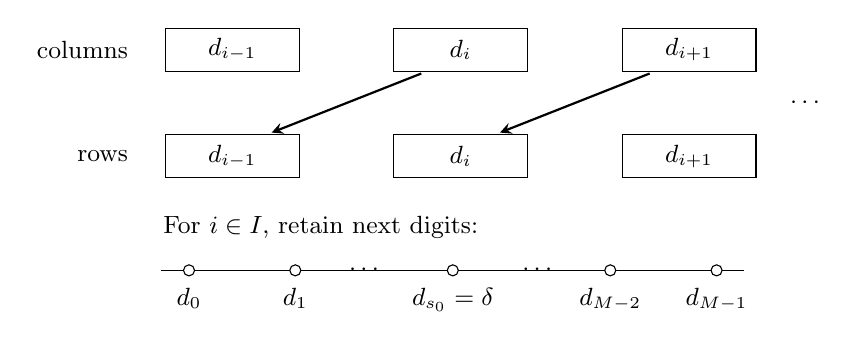
\begin{tikzpicture}[x=1cm,y=1cm,>=stealth,font=\small]
 \node[anchor=east] at (0,2.6) {columns};
 \node[anchor=east] at (0,1.25) {rows};
 \foreach \x/\lab in {1.2/{i-1},4.1/{i},7/{i+1}} {
   \node[draw,minimum width=1.7cm,minimum height=.55cm]
     at (\x,2.6) {$d_{\lab}$};
   \node[draw,minimum width=1.7cm,minimum height=.55cm]
     at (\x,1.25) {$d_{\lab}$};
 }
 \draw[->,thick] (3.6,2.3)--(1.7,1.55);
 \draw[->,thick] (6.5,2.3)--(4.6,1.55);
 \node at (8.5,1.93) {$\cdots$};
 \node[anchor=west] at (.2,.35)
   {For $i\in I$, retain next digits:};
 \draw (.3,-.2)--(7.7,-.2);
 \foreach \x/\lab in {.65/{d_0},2/{d_1},4/{d_{s_0}=\delta},6/{d_{M-2}},7.35/{d_{M-1}}} {
   \draw[fill=white] (\x,-.2) circle (2pt);
   \node[below] at (\x,-.3) {$\lab$};
 }
 \node at (2.9,-.2) {$\cdots$};
 \node at (5.1,-.2) {$\cdots$};
\end{tikzpicture}
\caption{One matching stage. Arrows show the first band of possible
pairings from a column cluster to the preceding row cluster; each
indicated cluster pair contains all lower-label pairs. In a retained
central cluster $i\in I$, the marked next digits have no pivot. The
spacings are schematic. The fixed-cut argument below uses the protected
digit $\delta=d_{s_0}$ to rule out crossings at sufficiently large
stages.}
\label{op:matching-figure}
\end{figure}

Fix now $J\in\Z$. At a sufficiently large stage, a possible matched
pair crossing $J$ would have column index
\[
 J<j\le J+X(1/M+2/p),
\]
since new matches occur only in the first band. Its lower label is
\[
 (\alpha+j)\bmod X=(X-1)/2+j
\]
without wrap, and its next digit is $\delta$. If the lower label is
eligible, its cluster index lies in $I$. In fact its representative
divided by $X$ differs from $1/2$ by at most
$1/M+2/p+o(1)$; if its last digit is $d_i$, the same representative
differs from $(i+1/2)/M$ by at most $1/p$. Hence $i$ is within three
places of $s_0$ for large $X$, which is inside $I$ since $M\ge81$.
But the next digit $\delta=d_{s_0}$ was explicitly retained there.
Such a pair cannot be matched. The remaining finitely many depths
each have only finitely many pairs crossing $J$. This proves the
first assertion.

For the second assertion, use labels with the prescribed units digit
and all later digits in $d(I)$ for columns or $d(I-1)$ for rows,
eventually all equal to $\delta$. These survive at every stage.
Changing finitely many digits of $\alpha$ gives an integer offset,
so each such label is $\alpha+j$ for a genuine integer row or
column index $j$. At a highest
modified position $r\ge1$, choose a center digit strictly below
$\delta$ for a column or strictly above it for a row. Both sets of
center digits contain such choices. The change at position $r$ has
absolute value at least $p^r$, while all lower changes together
have absolute value less than $p^r$, so this determines the
appropriate sign of the offset. The remaining $r-1$ intermediate digits can be
chosen freely, giving at least $B_0^{r-1}$ distinct offsets of
absolute value less than $p^{r+1}$. For $p^{r+1}\le N<p^{r+2}$,
these offsets lie in the required intervals and
\[
 B_0^{r-1}=p^{\beta(r-1)}\ge p^{-3\beta}N^\beta.
\]
Reducing the constant if necessary to work on both sides proves
the assertion for every sufficiently large integer $N$, including
cutoffs between successive powers of $p$.
\end{proof}

\section{From pivots to a gluing lattice}
\label{glue:section}

Fix the operator $a$ of Proposition~\ref{op:operator}. We first pass
from its finite-block pivots to actual kernel and cokernel vectors in
$\Phi$. The finite-crossing property makes the resulting quotient
Hausdorff and controls its compact open subspaces. We then pair the
two sorts of defects in a discrete lattice and glue it to the cone of
$a$. The resulting object will satisfy the first two conditions of
the transfer criterion; exclusion from $\Thick(T')$ will be the next
section's task.

For $J\in\Z$, put
\begin{equation}
 F_J\Phi=w^Jk[[w^{-1}]],\qquad
 \mathcal Q=\Phi/a\Phi,\qquad
 \mathcal K=\ker(a:\Phi\longrightarrow\Phi).
 \label{glue:spaces}
\end{equation}
The $F_J\Phi$ are compact open subspaces for the Laurent-series
topology, with $\Phi=\bigcup_JF_J\Phi$ and
$\bigcap_JF_J\Phi=0$. Give $\mathcal K$ the subspace topology and
$\mathcal Q$ the quotient topology. The \emph{leading position} of
a nonzero series is its greatest exponent of $w$.

The operator $a$ is continuous and preserves every $F_J\Phi$.
Consequently, for $L\le J$, its matrix block on indices
$L,\ldots,J$ is the induced map on the finite-dimensional space
$F_J\Phi/F_{L-1}\Phi$. This remains true for inputs with infinitely
many nonzero coefficients below $L$: their tails contribute nothing
to the displayed rows. The rank of this block is the
$\mathsf R(L,J)$ used in Lemma~\ref{op:matching}.

\begin{lemma}[Pivots and the pole topology]
\label{glue:pivot-topology}
An integer $j$ is an unmatched column of $a$ if and only if there is
a vector in $\mathcal K$ with leading term $w^j$. An integer $l$ is
a matched row if and only if it is the leading position of a nonzero
vector in $a\Phi$. Moreover, for every $J\in\Z$,
\begin{equation}
 \dim_k\frac{a\Phi\cap F_J\Phi}{a(F_J\Phi)}
   =\#\{(l,j)\text{ matched}:l\le J<j\}<\infty.
 \label{glue:crossing-quotient}
\end{equation}
The image $a\Phi$ is closed. Thus $\mathcal Q$ and $\mathcal K$ are
Hausdorff locally compact $k$-vector spaces, with compact open
subspaces given respectively by the images of $F_J\Phi$ and by
$\mathcal K\cap F_J\Phi$.
\end{lemma}

\begin{proof}
Suppose column $j$ is unmatched. For every lower cutoff $L\le j$,
its rank increment in the block $[L,j]$ is zero. Hence
\[
 S_L=\{f\in w^j+F_{j-1}\Phi:a(f)\in F_{L-1}\Phi\}
\]
is nonempty: a solution of the finite coefficient equations extends
by a zero tail. Continuity of $a$ makes $S_L$ closed in the compact
space $w^j+F_{j-1}\Phi$. Lowering $L$ adds equations, so these
sets are nested. Compactness gives a point in their intersection,
and its image lies in $\bigcap_LF_{L-1}\Phi=0$. This is an actual
kernel vector with leading term $w^j$. Conversely, such a vector
makes column $j$ dependent in every finite block, so the column is
unmatched. In particular,
\begin{equation}
 \dim_k\frac{a(F_j\Phi)}{a(F_{j-1}\Phi)}
 =
 \begin{cases}
 1,&\text{if column $j$ is matched},\\
 0,&\text{if column $j$ is unmatched}.
 \end{cases}
 \label{rew:glue:image-increment}
\end{equation}
Indeed, $F_j\Phi/F_{j-1}\Phi$ is generated by $w^j$, and
$a(w^j)\in a(F_{j-1}\Phi)$ is equivalent to the existence of the
kernel vector just constructed.

If row $l$ is matched, then at some finite column cutoff its
addition increases rank. A finite column combination therefore
has nonzero coefficient in that row and zero coefficients above
it. The combination is an actual Laurent polynomial input, and
triangularity makes all rows above the finite block vanish too.
Conversely, suppose $a(f)$ has leading position $l$. Write
$f=f_{\ge l}+f_{<l}$, where $f_{\ge l}$ is a Laurent polynomial
and $f_{<l}\in F_{l-1}\Phi$. Since $a$ preserves $F_{l-1}\Phi$,
the infinite tail contributes nothing on rows at least $l$.
The finite polynomial $f_{\ge l}$ therefore exhibits the same
row increment in a finite block, so row $l$ is matched.

For $J'>J$, equation~\eqref{rew:glue:image-increment} shows that
the dimension of $a(F_{J'}\Phi)/a(F_J\Phi)$ is the number of
matched columns in $(J,J']$. The map from this quotient to
$F_{J'}\Phi/F_J\Phi$ induced by projection has rank
$\mathsf R(J+1,J')$: the images of input terms at or below $J$
lie in $F_J\Phi$ and vanish under the projection. The kernel of
this induced map is
\[
 \frac{a(F_{J'}\Phi)\cap F_J\Phi}{a(F_J\Phi)}.
\]
Subtracting the projected rank therefore counts exactly the matches
with $l\le J<j\le J'$. Every Laurent input belongs to some
$F_{J'}\Phi$, so taking the increasing union over $J'$ proves
\eqref{glue:crossing-quotient}. This calculation precedes any
closedness assertion. The crossing count is finite by
Proposition~\ref{op:operator}.

The image $a(F_J\Phi)$ is compact by continuity. The quotient in
\eqref{glue:crossing-quotient} is finite-dimensional over the finite
field $k$, hence is a finite set. Thus $a\Phi\cap F_J\Phi$ is a
finite union of translates of $a(F_J\Phi)$, and is compact and
closed. The $F_J\Phi$ form an open cover of $\Phi$, so $a\Phi$ is
closed in $\Phi$. The quotient is Hausdorff, and the quotient map
is open, proving the asserted compact open subspaces of $\mathcal Q$.
The kernel is closed by continuity, and its intersections with the
compact open stages give the assertion for $\mathcal K$.
\end{proof}

\subsection{The complete cone and its overlap}

In the category of complete objects, or equivalently in the perfect
$\mathscr E$-module calculus of
Proposition~\ref{complete:realization}, define
\begin{equation}
 m=\cofib(a:\widehat T'\longrightarrow\widehat T'),
 \qquad Y=\bigoplus_{r=0}^{D-1}m[r].
 \label{glue:complete-object}
\end{equation}
Recall that $W_i(Y)=\pi_i LY$ denotes the normalized overlap.
The finite sum over all residues ensures that both kinds of defect
occur in every degree.

\begin{lemma}[Compact stages of the cone]
\label{glue:overlap}
For every degree $i$, the normalized overlap has an identification
\begin{equation}
 W_i(Y)=\mathcal Q\oplus\mathcal K,
 \label{glue:overlap-splitting}
\end{equation}
compatible with the $t$-period identifications. The map
$\pi_iY\longrightarrow W_i(Y)$ has finite kernel and compact open
image. Each such image is commensurable with
\begin{equation}
 C_0^{\rm lat}=\im_{\mathcal Q}(F_0\Phi)
                     \oplus(\mathcal K\cap F_0\Phi).
 \label{glue:standard-compact}
\end{equation}
The topology of $\pi_iY$ is the intrinsic compact topology from its
finite reductions, and the induced topology on the overlap is the
locally compact topology in \eqref{glue:overlap-splitting}. Every
fixed compact stage of this overlap is contained in the image of
one sufficiently late $t$-translated group $\pi_{i+sD}Y$.
\end{lemma}

\begin{proof}
The overlap of $\widehat T'$ is supported in degrees divisible by
$D$, with normalized coefficient space $\Phi$ and the action of $a$
used above. Since $D>2$, the cofiber calculation in each summand has
separate cokernel and kernel residues. In degree $i$, the cokernel
component comes from $m[r]$ with $i\equiv r\bmod D$, by the cofiber
inclusion from $\widehat T'[r]$. The kernel component comes from
$m[r']$ with $i\equiv r'+1\bmod D$, by the connecting map into
$\widehat T'[r'+1]$. Summing gives
\eqref{glue:overlap-splitting} and its periodic compatibility.

For complete homotopy, Proposition~\ref{complete:sections} replaces
$\Phi$ by the compact coefficient stages
\[
 (x^{-s}R)^\Lambda=F_{\lfloor s/q\rfloor}\Phi.
\]
The two components may use different values of $s$ and hence of $J$;
both increase without bound under positive $t$-translation.
On a cokernel component, the kernel of the map from the stage
cokernel to $\mathcal Q$ is exactly
$(a\Phi\cap F_J\Phi)/a(F_J\Phi)$, finite by
Lemma~\ref{glue:pivot-topology}; its image is the compact open image
of $F_J\Phi$. On a kernel component, the stage gives simply
$\mathcal K\cap F_J\Phi$, injecting into $\mathcal K$. This proves
the finite-kernel and compact-open claims. Any two compact open
subspaces here are commensurable: their intersection is open in each
compact space, so the two quotient spaces are finite.

By Lemma~\ref{complete:reductions}, the kernel and cokernel
calculations at a fixed compact stage are inverse limits of the
corresponding finite-level calculations. These inverse systems of
finite groups satisfy the Mittag--Leffler condition: at each fixed
level, their decreasing sequences of images stabilize. Their
inverse limits are therefore exact, and the resulting compact
topology is the intrinsic topology from reductions. Taking the
$t$-colimit recovers the same locally compact union topology on
$\mathcal Q\oplus\mathcal K$.
Finally the coefficient stages increase without bound under positive
$t$-translation. Choosing a single sufficiently large stage for both
components proves the last assertion.
\end{proof}

\subsection{A lattice pairing the defects}

We choose the open part by constructing, in each degree, a discrete
complement to the compact open subspace
$C_0^{\rm lat}\subset\mathcal Q\oplus\mathcal K$.
Such a complement can be obtained by lifting an algebraic basis of
$(\mathcal Q\oplus\mathcal K)/C_0^{\rm lat}$ and taking its span.
Adding a vector of $\mathcal K\cap F_0\Phi$ to the kernel coordinate
of a lift does not change its quotient class. We use this freedom to
attach the distinguished compact kernel vectors to independent polar
cokernel classes.

For each forever unmatched positive row $j$, let $q_j\in\mathcal Q$
be the class of $w^j$. For each forever unmatched nonpositive column
$l$, choose $k_l\in\mathcal K$ with leading term $w^l$, as supplied
by Lemma~\ref{glue:pivot-topology}. In particular
$k_l\in\mathcal K\cap F_0\Phi\subset R$. Pair these lists in order
of increasing $j$ and increasing $|l|$; write $(j,l)$ for a resulting
pair of an unmatched row and an unmatched column.
Since $(0,k_l)\in C_0^{\rm lat}$, the pair $(q_j,k_l)$ and the
vector $(q_j,0)$ have the same image in the quotient. The next lemma
verifies the independence of these quotient classes and records
simultaneous bounds on their leading positions.

\begin{lemma}[Simultaneous defect pairs]
\label{glue:pairs}
The vectors $(q_j,k_l)\in\mathcal Q\oplus\mathcal K$, indexed by
the paired lists, are linearly independent modulo $C_0^{\rm lat}$.
For every sufficiently large integer $N$, at least $cN^\beta$ pairs,
for a fixed $c>0$, simultaneously satisfy $j\le N$ and $|l|\le N$.
For these pairs, their kernel coordinates are linearly independent
modulo $x^{qN+1}R$.
\end{lemma}

\begin{proof}
The $q_j$ are independent modulo $\im_{\mathcal Q}(F_0\Phi)$.
Otherwise a finite nontrivial relation, after subtracting a vector in
$F_0\Phi$, would be an actual image of $a$ whose leading position
is an unmatched positive row. This contradicts
Lemma~\ref{glue:pivot-topology}. It also proves independence of the
pairs modulo $C_0^{\rm lat}$.

Let $n_+(N)$ count the positive unmatched rows at most $N$, and let
$n_-(N)$ count the nonpositive unmatched columns of absolute value
at most $N$. In the ordered pairing, the first condition holds
precisely for the first $n_+(N)$ pairs and the second for the first
$n_-(N)$ pairs. Thus exactly $\min\{n_+(N),n_-(N)\}$ pairs satisfy both
conditions. Proposition~\ref{op:operator} bounds each count below
by a constant times $N^\beta$ for every sufficiently large $N$,
giving the simultaneous bound.
The leading terms of their kernel vectors are the distinct powers
$w^l=x^{q|l|}$, with $q|l|\le qN$. A nonzero combination has one of
these as its lowest $x$-power, so cannot lie in $x^{qN+1}R$.
\end{proof}

In every period residue, extend the independent images of the pairs
to an algebraic basis of
$(\mathcal Q\oplus\mathcal K)/C_0^{\rm lat}$. Choose lifts retaining
the specified pairs, and let $\mathcal L_i$ be their span. The
projection of this algebraic span to the quotient is an isomorphism.
It therefore meets $C_0^{\rm lat}$ trivially and, together with
$C_0^{\rm lat}$, fills the whole space. Since $C_0^{\rm lat}$ is
open, the span is discrete. Each open coset of $C_0^{\rm lat}$
contains exactly one point of the span, so the span is also closed.
Finally, the compact space $C_0^{\rm lat}$ maps onto the quotient
by the span, proving cocompactness. Make the same choice along each
$t$-period.

By Lemma~\ref{complete:open-splitting}, the $t$-open category is
the split category of $D$-periodic complexes of $k$-vector spaces.
There is consequently an open object $V$, also regarded as pushed
forward to $\mathbf D(\mathcal N)$, and a map $V\to LY$ whose maps
on homotopy are precisely these lattice inclusions. Define
\begin{equation}
 U=Y\mathop{\times}_{LY}V\quad\text{in }\mathbf D(\mathcal N),
 \label{glue:definition-U}
\end{equation}
where the pullback is a homotopy pullback.

\begin{proposition}[The glued object]
\label{glue:object}
The object $U$ of \eqref{glue:definition-U} satisfies
\[
 \pi_iU\text{ is finite for every }i,\qquad
 \widehat U\simeq Y\in\Thick(\widehat T'),\qquad LU\simeq V.
\]
Under these equivalences the structure map
$LU\longrightarrow L\widehat U$ is the chosen lattice map.
\end{proposition}

\begin{proof}
By Lemma~\ref{glue:overlap}, the map from $\pi_iY$ to $\pi_iLY$
has finite kernel and compact open image; call this image $C_i$.
It is commensurable with $C_0^{\rm lat}$, and
$\pi_iV=\mathcal L_i$ is a discrete complement to
$C_0^{\rm lat}$. Consider the joint map
\[
 \pi_iY\oplus\pi_iV\longrightarrow\pi_iLY.
\]
After dividing its kernel by the finite kernel of $\pi_iY\to C_i$,
one obtains $C_i\cap\mathcal L_i$. This intersection injects into
$C_i/(C_i\cap C_0^{\rm lat})$, which is finite. The cokernel of the
joint map is a quotient of
$C_0^{\rm lat}/(C_i\cap C_0^{\rm lat})$, also finite.
Thus the joint map has finite kernel and cokernel in every degree.
The pullback long exact sequence expresses $\pi_iU$ as an extension
of the kernel in degree $i$ by the cokernel in degree $i+1$.
Both are finite, so $\pi_iU$ is finite.

Both $V$ and $LY$ are $t$-invertible and hence have zero completion.
Exactness of completion and completeness of $Y$ give
$\widehat U\simeq Y$. Localizing the pullback instead gives
$LU\simeq V$, since the localization of $Y\to LY$ is an equivalence.
These identifications preserve the structure map. The object $Y$ is
a finite sum of shifts of a two-cell cone on $\widehat T'$, so lies
in $\Thick(\widehat T')$.
\end{proof}

The construction has now supplied the finite homotopy and complete
thick-membership parts of Proposition~\ref{transfer:criterion}.
The following consequence of the chosen lattice is the restriction
that will obstruct global thick membership.

\begin{lemma}[Constraint on global maps]
\label{glue:global-maps}
For every map $g:U\to P$ with $P\in\Thick(T')$, the induced map
\[
 W_i(\widehat g):\mathcal Q\oplus\mathcal K
                    \longrightarrow W_i(\widehat P)
\]
is continuous and sends each paired vector $(q_j,k_l)$ into the
discrete lattice $\im(\pi_iLP\to W_i(\widehat P))$.
\end{lemma}

\begin{proof}
Objects of $\Thick(T')$ have finite homotopy in each degree. The
same is true of $U$ by Proposition~\ref{glue:object}.
Proposition~\ref{complete:topology} therefore makes every map between
their completions continuous on overlap homotopy. Under
Lemma~\ref{glue:overlap}, the source topology is precisely the
locally compact topology on $\mathcal Q\oplus\mathcal K$ used here.

The additional lattice assertion uses that $\widehat g$ comes from
the global map $g$. Naturality of the fracture square gives a
commutative square from $LU\to L\widehat U$ to
$LP\to L\widehat P$. Each paired vector is represented in
$\pi_iLU=\pi_iV=\mathcal L_i$. Applying $\pi_iLg$ and then the
target structure map places its image in
$\im(\pi_iLP\to W_i(\widehat P))$, which is the discrete lattice
provided by Proposition~\ref{complete:topology}. This argument
uses the representative in $\pi_iLU$; an individual pair need not
lift to $\pi_iU$.
\end{proof}

To see how the pairing will be used, choose a compact open target
subspace containing the images of the kernel coordinates. Modulo
this subspace, each paired image is its polar image. Since all paired
images lie in a discrete lattice, the part of their span inside the
compact subspace has finite dimension. Thus a rank bound for the
polar images controls the rank of the paired images up to a fixed
finite error. The next section obtains the required bound under its
homology-vanishing hypothesis.

\section{The obstruction to a global finite construction}
\label{obs:section}

The object $U$ of Proposition~\ref{glue:object} has finite homotopy
groups in every degree, and its completion is the finite construction
\[
 Y=\bigoplus_{r=0}^{D-1}m[r],\qquad
 m=\cofib\bigl(a:\widehat T'\longrightarrow\widehat T'\bigr).
\]
The remaining condition in the transfer criterion is
$U\notin\Thick(T')$.  We must rule out every finite tower of shifts
of $T'$ and every retract of such a tower.  Ruling out a retract
of a finite sum of shifts would still leave longer towers untreated.

We first isolate the finite-tower argument.  Its input is an exact
functor to perfect modules over a periodic algebra over a domain
with principal left and right ideals.  The criterion uses ordinary
homology and the homology of module duals
to pass backward through any finite tower: the dual test removes
the free part of a tower tail, and the ordinary test then uses
torsion to force vanishing.  We next construct a flat extension of
the operation coefficients for which $Y$ has nonzero torsion
homology.  The final part verifies the relation between the two
tests for maps that come from global objects.

\subsection{A criterion for arbitrary finite constructions}

We state the two tests abstractly before constructing the
coefficient extension that will make them apply to the operator
$a$ and the gluing lattice.  Torsion homology by itself
cannot be the obstruction: the cone of $2:\Z\to\Z$ is a two-cell
object with homology $\Z/2$.  The additional information will
restrict the maps that exist in the original category.

Let $\mathscr B_0=S_0[t^{\pm1}]$, where $S_0$ is a domain with principal
left and right ideals, $t$ is central of positive even homological
degree $D_0$, and the differential is zero.  Write $\Perf(\mathscr B_0)$
for the full subcategory of the derived category consisting of
perfect right dg $\mathscr B_0$-modules.
For a right module over a domain, we call an element \emph{torsion}
if it is annihilated on the right by a nonzero ring element.  In the
principal domains used below the Ore property makes these elements
a submodule.  A torsion module has no nonzero map to a free module:
the image of a torsion element would be annihilated by a nonzero
element of the domain.

For $M\in\Perf(\mathscr B_0)$ its module dual is the left dg module
\[
 M^*=R\Hom_{\mathscr B_0}(M,\mathscr B_0).
\]
A map $f:M\to N$ induces
$H(f):H(M)\to H(N)$ and
$H(f^*):H(N^*)\to H(M^*)$.  The dual test has the opposite
direction, and in both tests vanishing means zero in every degree.

Testing finite constructions by maps invisible to homology is part
of the theory of ghosts and projective classes developed by
Christensen~\cite[Theorem~3.5 and Section~8]{Christensen1998}.
The following criterion adds a relation between the two tests for
maps in the original category.  Its proof is included.

\begin{theorem}[A finite-tower criterion]
\label{rew:obs:tower-criterion}
Let $\mathcal C$ be an idempotent-complete triangulated category,
let $T_0,U_0\in\mathcal C$, and let
\[
 \Psi:\mathcal C\longrightarrow\Perf(\mathscr B_0)
\]
be an exact functor with $\Psi(T_0)\simeq\mathscr B_0$.  Assume that
$H(\Psi(U_0))$ is torsion as a right $S_0$-module in every degree
and is nonzero in at least one degree.  Assume also that, for every
$P\in\Thick_{\mathcal C}(T_0)$ and every map $g:U_0\to P$ in
$\mathcal C$,
\begin{equation}
\label{rew:obs:two-tests}
 H(\Psi(g))=0
 \quad\Longrightarrow\quad
 H\bigl((\Psi(g))^*\bigr)=0.
\end{equation}
Then $U_0\notin\Thick_{\mathcal C}(T_0)$.
\end{theorem}

Here $\Thick_{\mathcal C}(T_0)$ is the ordinary thick closure,
using isomorphisms, finite sums, all integer shifts, triangles
and retracts.
The quantifier in \eqref{rew:obs:two-tests} concerns maps in
$\mathcal C$.  In our application, their global origin is precisely
what imposes a constraint on the gluing lattice.

The proof uses two algebraic facts.  The first separates free
homology from torsion homology over the coefficient ring.

\begin{lemma}[Periodic splitting]
\label{obs:periodic-splitting}
Let $S_0$ be a domain whose left and right ideals are principal, and
let $D_0$ be a positive even integer.  Every finitely generated right
$S_0$-module is a direct sum of a torsion module and a finite free
module and has a finite free resolution of length at most one.
Every perfect right dg module over
$S_0[t^{\pm1}]$, with $|t|=D_0$ and zero differential, splits in its
derived category into the $D_0$-periodizations of its shifted homology
modules.  In particular it splits as a finite sum of free shifts and
a perfect module with torsion homology.
\end{lemma}

\begin{proof}
First, $S_0$ is noetherian on both sides, since every one-sided
ideal is principal.  Nonzero right ideals $dS_0$ and $eS_0$ must
intersect.  Otherwise the right ideals $e^i dS_0$, $i\geq0$,
would form an infinite internal direct sum in $S_0$: in a finite
relation, its term of least $e$-power belongs both to $dS_0$ and
to $eS_0$ after canceling that power, and hence vanishes; continue
inductively.  This contradicts noetherianity.  The same argument
on the left gives the two-sided Ore division ring of fractions
$Q_0$.  Clearing common
denominators gives exact localization of modules.  Consequently,
for a finitely generated right module $M$, the kernel
\[
 M_{\mathrm{tor}}=\ker\bigl(M\longrightarrow M\otimes_{S_0}Q_0\bigr)
\]
consists exactly of the elements right-annihilated by a nonzero
element of $S_0$.

The quotient $M/M_{\mathrm{tor}}$ embeds in the finite-dimensional
right $Q_0$-vector space $M\otimes_{S_0}Q_0$.  Choose coordinates
in that space and finitely many generators of the embedded module.
In each coordinate, clear their common \emph{left} denominators.
Left multiplication in a coordinate is right $S_0$-linear, so this
produces an injection
\[
 M/M_{\mathrm{tor}}\longrightarrow S_0^r
\]
for some finite $r$.  The choice of left denominators is the one
compatible with right modules.

Every submodule of $S_0^r$ is free of finite rank.  To prove this,
induct on $r$ and project to the first coordinate.  The image is
a right ideal.  If it is zero, the induction hypothesis applies
inside $S_0^{r-1}$.  If it is nonzero, its principal generator is
a nonzero element of the domain, so the image is free of rank one.
The projection then splits, and its kernel lies in $S_0^{r-1}$.
This proves the assertion in both cases.  It follows that
$M/M_{\mathrm{tor}}$ is finite free, and hence that the sequence
with this quotient splits.  The kernel of a finite free presentation
of $M$ is also finite free by the same argument.  This gives a
finite free resolution of length at most one.

Now view a dg module over $S_0[t^{\pm1}]$ as a $D_0$-periodic
complex of right $S_0$-modules.  A finite-cell module has finite
free modules in each period residue, and noetherianity of $S_0$
makes its homology finitely generated there.  The same holds for
a retract, hence for every perfect module $P$.
For each $i\in\{0,\ldots,D_0-1\}$ choose a resolution
\[
 0\longrightarrow R_{1,i}\longrightarrow R_{0,i}
   \longrightarrow H_i(P)\longrightarrow0
\]
by finite free right modules.  Place $R_{0,i}$ in degree $i$ and
$R_{1,i}$ in degree $i+1$.  Lift the free generators of $R_{0,i}$
to cycles in a representative complex for $P$.  The images of
the relations are boundaries.  Since $R_{1,i}$ is free, lift them
through the differential onto the boundaries in degree $i$.
This gives a map of the two-term complex into $P$.

Extend the map periodically using multiplication by $t$.
The positive even degree $D_0$ gives the usual periodization
without changing the homological signs.  This periodized complex
has homology $H_i(P)$ in residue $i$ and zero in the other residues.
Sum the maps over $0\leq i<D_0$.  The sum is finite and induces
an isomorphism in every homology degree, so it is a
quasi-isomorphism.  Finally split each $H_i(P)$ into its torsion
and finite free parts.  The periodizations of the free parts are
finite sums of free shifts; those of the torsion parts are perfect
because of their length-one finite free resolutions.  This gives
the asserted splitting.
\end{proof}

The second puts every finite construction into a tower of free
layers, with all retracts taken at the end.

\begin{lemma}[Finite towers and retracts]
\label{rew:obs:tower-normal-form}
For an idempotent-complete triangulated category $\mathcal C$ and
an object $T_0$, every $P\in\Thick_{\mathcal C}(T_0)$ is a
retract of an object $P_0$ admitting a finite tower of triangles
\[
 F_j\longrightarrow P_j\longrightarrow P_{j+1}
      \longrightarrow F_j[1],
 \qquad 0\leq j<s,\qquad P_s=0,
\]
where each $F_j$ is a finite sum of arbitrary integer shifts of
$T_0$.
\end{lemma}

\begin{proof}
Call an object a finite extension of free layers if it admits such
a tower.  Zero, finite sums of shifts of $T_0$, and their shifts
have this property.  The octahedral axiom concatenates two towers.
More explicitly, suppose $A\to E\to B$ is a triangle, and the
first layer of a tower for $A$ is $F_0\to A\to A_1$.  The cofiber
$E_1$ of the composite $F_0\to A\to E$ fits into triangles
\[
 F_0\longrightarrow E\longrightarrow E_1,
 \qquad A_1\longrightarrow E_1\longrightarrow B.
\]
Induction on the number of layers in $A$, ending with the tower
for $B$, gives a tower for $E$.  In particular, if $A$ and $B$
have towers and $f:A\to B$ is a map, the triangle
\[
 B\longrightarrow\cofib(f)\longrightarrow A[1]
\]
gives a tower for $\cofib(f)$.  Finite sums of towers give the
same closure for finite sums.

It remains to move retracts to the end.  Let $A$ and $B$ be
retracts of finite extensions $\overline A$ and $\overline B$.
Idempotent completeness supplies complements
\[
 \overline A\simeq A\oplus A',
 \qquad \overline B\simeq B\oplus B'.
\]
Extend a map $f:A\to B$ to
$\overline f:\overline A\to\overline B$ by setting all other
matrix entries to zero.  Its cone is isomorphic to
\[
 \cofib(f)\oplus B'\oplus A'[1].
\]
Thus $\cofib(f)$ is a retract of a finite extension.  Shifts,
finite sums and successive retracts of such objects are also
retracts of finite extensions.  The resulting subcategory is thick
and contains $T_0$, which proves the lemma.
\end{proof}

\begin{proof}[Proof of Theorem~\ref{rew:obs:tower-criterion}]
Suppose that $U_0\in\Thick_{\mathcal C}(T_0)$.
By Lemma~\ref{rew:obs:tower-normal-form}, choose a retract
insertion $g_0:U_0\to P_0$ and a tower as in that lemma.
Let $g_j:U_0\to P_j$ be the composite with the map to its
$j$th tail, and put $Y_0=\Psi(U_0)$.
We prove backward from $j=s$ that
\[
 H(\Psi(g_j))=0,
 \qquad H\bigl((\Psi(g_j))^*\bigr)=0.
\]
Both assertions hold for $P_s=0$.

Write one extended step as
\[
 F\longrightarrow P_1'\longrightarrow P_2'
      \longrightarrow F[1],
 \qquad g_1':Y_0\to P_1',\quad g_2':Y_0\to P_2',
\]
where $F$ is a finite sum of free shifts, and suppose that the
two vanishing assertions hold for $g_2'$.
By Lemma~\ref{obs:periodic-splitting}, choose
\[
 P_2'\simeq V'\oplus L',
\]
with $V'$ a finite sum of free shifts and $H(L')$ torsion.
Each component of the projection $P_2'\to V'$ is a class in
the homology of $(P_2')^*$.  Dual-homology vanishing for $g_2'$
says that its composite with each of these classes is zero.
Hence
\[
 Y_0\xrightarrow{g_2'}P_2'\longrightarrow V'
\]
is zero as a derived map.  The exact sequence of maps into the
fiber triangle therefore lifts $g_1'$ to
\[
 Z'=\fib(P_1'\longrightarrow V').
\]
The fiber construction, equivalently the octahedral axiom, gives
a triangle
\[
 F\longrightarrow Z'\longrightarrow L'\longrightarrow F[1].
\]

In its homology sequence, the map preceding
$H(F)\to H(Z')$ has torsion source and free target in each
degree.  It is zero, so $H(F)\to H(Z')$ is injective.
The lifted map $Y_0\to Z'$ is zero on homology after composition
with $Z'\to L'$, because that composite is the corresponding
summand of $g_2'$.  Its homology therefore factors through
the submodule $H(F)\subset H(Z')$.  The source $H(Y_0)$ is
torsion, so its map into the free module $H(F)$ is zero.
It follows that $H(g_1')=0$.

The map $g_1'$ is the image of a map $U_0\to P_j$ in
$\mathcal C$, and this tower tail belongs to
$\Thick_{\mathcal C}(T_0)$.  Hypothesis
\eqref{rew:obs:two-tests} gives $H((g_1')^*)=0$ as well.
This completes the backward induction.  In particular
$\Psi(g_0)$ is zero on homology.  It has a left inverse because
$g_0$ is a retract insertion and every functor preserves its
retraction equation.  Thus $H(\Psi(g_0))$ is also a split
injection, contradicting the nonzero homology of $Y_0$.
\end{proof}

The two tests have distinct roles in the induction.  Dual homology
removes the free quotient of a tower tail as an actual derived map.
Ordinary homology then places the remaining map in a free submodule,
where torsion forces it to vanish.  The implication
\eqref{rew:obs:two-tests} restores the dual statement for the next
step.  There is no bound on the length of the proposed tower.

\subsection{A flat coefficient extension}

We now construct the coefficient ring required by the criterion.
The extension must be flat on both sides: homology of right
modules and homology of their left-module duals will both be tested
after extending coefficients.  It must also keep the cone of $a$
nonzero while making its homology torsion.

There are two filtrations in what follows.  The paired vectors in
$W_i(Y)=\mathcal Q\oplus\mathcal K$ have Laurent pole bounds in
$K_0=k((x))$.  The operation ring $\Delta=R[[H]]$, with $R=k[[x]]$,
has instead the weight filtration of
Proposition~\ref{geom:skew-filtration}, with
\[
 \gr\Delta=k[\sigma x,A,B,C],\qquad
 |\sigma x|=4,\quad |A|=|B|=1,\quad |C|=3.
\]
The coefficient extension will be taken at the homogeneous prime
$(C)$ and used only to test homology of perfect modules.  The later
estimate concerns integral operators acting on
Laurent functions: it compares the growth of their joint kernels
with the larger exponent $\beta>1/3$ supplied by
Lemma~\ref{glue:pairs}.

We give the filtered algebra argument with explicit hypotheses.  A
decreasing filtration is indexed by integers and is multiplicative.  Its
initial-symbol map is denoted by $\sigma$.  A filtration on a finitely
generated module is called \emph{good} if it is the quotient filtration
from a finite direct sum of filtration shifts of the ring.
The construction through truncated Rees rings is the algebraic approach
to microlocalization developed by Asensio, Van den Bergh, and
Van Oystaeyen~\cite[Sections~2--3]{AVVO1989}.  We give the construction
and flatness argument in the precise complete setting needed here.

\begin{lemma}[Filtered microlocalization]
\label{obs:microlocal-flat}
Let $k$ be a finite field, and let $\mathcal A$ be a complete separated
filtered $k$-algebra such that $F^n\mathcal A=\mathcal A$ for $n\leq0$
and
\[
 \gr\mathcal A=k[z_1,\ldots,z_d,c]
\]
as a graded algebra, with all the displayed generators of positive
integer degree.  There is a filtered algebra $\mathcal S$ and a map
$\mathcal A\to\mathcal S$ with the following properties:
\begin{enumerate}
 \item $\gr\mathcal S$ is the homogeneous localization of
 $\gr\mathcal A$ obtained by inverting all homogeneous elements outside
 $(c)$;
 \item $\mathcal S$ is separated and complete for its exhaustive
 filtration, which is allowed to have nonzero terms of negative degree;
 \item $\mathcal S$ is flat as both a left and a right
 $\mathcal A$-module.
\end{enumerate}
For a finitely generated good filtered right module $M$, the corresponding
microlocalized module is $M\otimes_{\mathcal A}\mathcal S$ and its
associated graded is the same homogeneous localization of $\gr M$.
The analogous assertion holds for left modules.
\end{lemma}

\begin{proof}
We first justify the finite-module filtration properties needed for the
construction.  If $N$ is a submodule of a finite shifted filtered free
module, choose homogeneous generators of $\gr N$ over the noetherian
ring $\gr\mathcal A$ and lift them to $N$.  For an element of $N$,
subtract a linear combination of the lifts matching its initial symbol,
and repeat.  The remainder increases in filtration at each step.
The coefficients of each chosen lift form a convergent series in
$\mathcal A$, so the element is a finite linear combination of the
lifts.  This also proves that the resulting surjection from a finite
shifted free module is strict for the induced filtration.

Each quotient $\mathcal A/F^n\mathcal A$ is finite: the graded pieces
below $n$ are finite-dimensional over the finite field $k$.
Consequently $\mathcal A$ and its finite products are compact.
The submodule just considered is therefore compact and closed, being
the image of a compact finite free module.  Notice that closedness was
not assumed during the initial-symbol subtraction.  These observations
prove that $\mathcal A$ is noetherian on both sides and that every
finitely generated module has a complete separated good filtration.
Submodule and quotient filtrations are good, by using their preimages
in a finite free presentation.  A map of finite good filtered modules
is bounded up to a filtration shift, as one sees on strict generators.
In particular, any two good filtrations on one module differ by bounded
shifts.

Form the Rees ring and Rees module
\[
 \widetilde{\mathcal A}
   =\bigoplus_{n\in\mathbb Z}F^n\mathcal A\,s^{-n},
 \qquad
 \widetilde M
   =\bigoplus_{n\in\mathbb Z}F^nM\,s^{-n},
\]
where $s$ is central of Rees degree $-1$.
For $j\geq1$, work modulo $s^j$ and invert the homogeneous elements
whose reductions modulo $s$ lie outside $(c)$.
Such elements are regular, by induction through the $s$-layers and
regularity of their nonzero reductions in the polynomial ring.
They satisfy the Ore conditions on both sides.  Indeed all commutators
are divisible by $s$, so for a denominator $d$ and an element $e$ one
has $\operatorname{ad}_d^j(e)=0$ modulo $s^j$.  Expanding this identity
shows that $d^j e$ has a right factor $d$, and that $e d^j$ has a left
factor $d$.  Powers of a denominator are still denominators.  These
relations give the Ore conditions first for homogeneous elements and
then for their finite sums.  We may thus use ordinary two-sided Ore
localization, retaining the Rees grading.  Localization is exact on
modules, by clearing common denominators.

Let $M_j^\mu$ denote this localization of
$\widetilde M/s^j\widetilde M$.  Denominators lift across truncation
levels.  The localizations therefore reduce compatibly, and localizing
a module from a lower level at a higher level gives its own
localization.  Define
\begin{equation}
\label{obs:mu-definition}
 F^n\mu(M)=\lim_j(M_j^\mu)_n,
 \qquad
 \mu(M)=\bigcup_{n\in\mathbb Z}F^n\mu(M).
\end{equation}
The inclusions in this union come from multiplication by powers of $s$.
More precisely, regularity of $s$ on the untruncated Rees module gives,
after exact localization,
\begin{equation}
\label{obs:rees-layers}
 0\longrightarrow(M_j^\mu)_{n+l}
 \xrightarrow{\ s^l\ }(M_{j+l}^\mu)_n
 \longrightarrow(M_l^\mu)_n\longrightarrow0
 \qquad(l,j\geq1).
\end{equation}
Transitions in each fixed Rees degree are surjective.  Taking limits
in \eqref{obs:rees-layers} gives the asserted inclusions and
\[
 F^n\mu(M)/F^{n+l}\mu(M)=(M_l^\mu)_n.
\]
The filtration is separated and complete.  In fact compatible Cauchy
data eventually lie in one fixed $F^n\mu(M)$, where both assertions
follow from the inverse-limit description.  Taking $l=1$ identifies
the associated graded with the homogeneous localization of $\gr M$.

Products at the truncated levels give
$\mathcal S=\mu(\mathcal A)$ its ring structure and give $\mu(M)$
its module structure.  The natural maps from $\mathcal A$ and $M$
are obtained by taking their classes at each level.  A bounded-shift
map of good filtered modules gives a map on these unions; changing
the bound does not change the map, by the transition inclusions.
Thus the underlying module $\mu(M)$ is functorial and independent
of the good filtration chosen.

This functor is exact on finite modules.  Use induced and quotient
filtrations in a short exact sequence to make it strict.  Its Rees
sequence remains exact modulo $s^j$, because the quotient Rees module
is $s$-torsion-free.  Ore localization preserves exactness.  Inverse
limits preserve it here because the transition maps in each module
system are surjective, and taking the filtered union preserves it as
well.  The natural map
\[
 M\otimes_{\mathcal A}\mathcal S\longrightarrow\mu(M)
\]
is an isomorphism for a free module and hence for every finite module
by a finite presentation.  This proves left flatness of $\mathcal S$;
over a noetherian ring, exactness on finite modules suffices for this
flatness test.  The identical construction for left modules proves
right flatness.
\end{proof}

Apply Lemma~\ref{obs:microlocal-flat} to $\mathcal A=\Delta$ and
$c=C$, and write $S$ for the resulting ring.  The initial symbol of
$x$ is a unit in $\gr S$.  Lifting its inverse and correcting the
successive errors in increasing filtration shows that $x$ is a unit
in $S$.  Both left and right flatness hold also over $\Delta[x^{-1}]$:
on a module over that ring, balancing by the invertible $x$ identifies
tensoring over $\Delta$ with tensoring over $\Delta[x^{-1}]$.

Recall from Proposition~\ref{complete:operations} that
\[
 \mathscr E[t^{-1}]=A_{\mathrm{op}}[t^{\pm1}],
 \qquad A_{\mathrm{op}}=(\Delta[x^{-1}])^\Lambda.
\]
The tame character decomposition makes $\Delta[x^{-1}]$ finite free
over $A_{\mathrm{op}}$ on either side.  Indeed $x$ has a faithful
$\Lambda$-character and is a unit; multiplication on either side
by its powers identifies every character space with the invariant
space.  We have proved the following coefficient-extension statement:
\begin{equation}
\label{obs:coefficient-extension}
 \mathscr E\longrightarrow
 A_{\mathrm{op}}[t^{\pm1}]
 \longrightarrow\Delta[x^{-1}][t^{\pm1}]
 \longrightarrow\mathscr B:=S[t^{\pm1}]
\end{equation}
is flat on both sides.  Here $t$ is central, of homological degree $D$;
$S$ is in homological degree zero and has zero differential.
The filtration on $S$ is unrelated to this homological grading.

The following lemma verifies the remaining ring properties and
shows that the cone of $a$ retains nonzero torsion homology.

\begin{lemma}
\label{obs:principal}
The ring $S$ is a domain, every left or right ideal of $S$ is principal,
and $S$ has a two-sided Ore division ring of fractions.  The operator
$a$ constructed in Proposition~\ref{op:operator} has no one-sided inverse
in $S$.  In particular $S/aS\ne0$, and this right $S$-module is torsion.
\end{lemma}

\begin{proof}
The graded ring of $S$ is a domain, so multiplicativity of initial
symbols proves that $S$ is a domain.  Every nonzero homogeneous element
of $\gr S$ is a power of $C$ times a homogeneous unit.  In a nonzero
right ideal choose $d_0$ minimizing the nonnegative $C$-order of its
initial symbol.  For any member $d$ of the ideal, its initial symbol
is a multiple of $\sigma(d_0)$.  Lift the multiplier and subtract the
corresponding right multiple of $d_0$.  The remainder is still in the
ideal and has strictly larger filtration, so its initial $C$-order
is still at least the chosen minimum.  Repeating, and summing the
convergent multipliers, expresses $d$ as a right multiple of $d_0$.
The successive multipliers tend to zero because their filtration
degrees increase by the same amount as those of the remainders.
This proves the right principal-ideal property; the left proof is
identical.

The intersection argument in the proof of
Lemma~\ref{obs:periodic-splitting} now gives the two-sided Ore
division ring of fractions.

The operator $a$ still has initial symbol $C$ in $S$.  A one-sided
inverse would make $C$ invertible in $\gr S$, which it is not.
Thus $S/aS\ne0$.  Given a nonzero representative $b\in S$, the
nonzero intersection $bS\cap aS$ supplies a nonzero $d$ with
$bd\in aS$.  Every class in $S/aS$ is therefore annihilated on the
right by a nonzero element, proving torsion.
\end{proof}

\paragraph{The instance supplied by the glued object.}
We now return to $\mathbf D(\mathcal N)$ and the coefficient
extension \eqref{obs:coefficient-extension}.  Let
\[
 \mathcal C_{\mathrm{comp}}
 =\{P\in\mathbf D(\mathcal N):
       \widehat P\in\Thick(\widehat T')\}
\]
be the full subcategory with the displayed property.
Completion is exact by Proposition~\ref{complete:fracture}, so
the inverse image of $\Thick(\widehat T')$ is thick.  The ambient
derived category is idempotent-complete, and the defining property
is closed under retracts; hence $\mathcal C_{\mathrm{comp}}$ is
idempotent-complete as well.  It contains $T'$, and
it contains $U$ because Proposition~\ref{glue:object} identifies
$\widehat U$ with the displayed finite construction $Y$.
Compose completion, the inverse of the strict realization
equivalence in Proposition~\ref{complete:realization}, and derived
extension of scalars to obtain an exact functor
\[
 \Psi:\mathcal C_{\mathrm{comp}}\longrightarrow\Perf(\mathscr B).
\]
We write $\widehat P_{\mathscr B}$ for $\Psi(P)$ and use the
same subscript for the image of a map.  The functor sends $T'$
to the free right module $\mathscr B$.

On a free right module, the map determined by $1\mapsto a$ is
left multiplication by $a$.  It is injective over $S$ because
$S$ is a domain, and its cokernel is the right module $S/aS$.
Since $Y$ is the sum of all $D$ shifts of this cone,
\begin{equation}
\label{rew:obs:source-homology}
 H_i(\Psi(U))\cong S/aS
 \quad\text{as right $S$-modules for every integer }i.
\end{equation}
Lemma~\ref{obs:principal} says that this module is nonzero and
torsion.  This verifies the first hypothesis of
Theorem~\ref{rew:obs:tower-criterion}.  The remaining task is
the implication from homology vanishing to dual-homology
vanishing for every global map $g:U\to P$ with
$P\in\Thick_{\mathbf D(\mathcal N)}(T')$.

\subsection{A growth bound for joint operator kernels}

To prove the remaining implication, we return to integral operators
acting on $K_0=k((x))$.  For the remainder of this section let
$\bar b$ denote the reduction of $b\in\Delta$ in
$\Omega=\Delta/(x)=k[[H]]$.  The notation $\sigma(\bar b)$ means
the subsequent initial symbol for the weight filtration on
$\Omega$; reduction modulo $x$ and passage to the initial symbol
are distinct operations.
The congruence subgroups $H_l$, their indices $N_l$, and the balanced
sequence $b_j^H$ are those used in
Lemma~\ref{op:displacement} and
Lemma~\ref{op:divided-differences}.  In particular, with
$z_h=h(x)/x$, we have
\begin{equation}
\label{obs:growth-inputs}
 r'_m=\sum_{l\geq1}\lfloor m/N_l\rfloor\leq\kappa m,
 \qquad
 \Gamma_s\subset H_{p^s},\qquad
 N_{p^s}\geq p^{3(s-1)}\quad(s\geq1).
\end{equation}
These are the inputs that will turn linear Laurent precision into
cubic-root dimension growth.

\begin{lemma}[Joint-kernel growth]
\label{obs:growth}
Suppose $a_1,b_1\in\Delta$ satisfy
\[
 \bigl(\sigma(\bar a_1)\bigr)=(C)
 \quad\text{in }\gr\Omega=k[A,B,C],
 \qquad \sigma(\bar b_1)\notin(C).
\]
Fix an integer $L_0\geq0$.  There is a constant $c_0$, depending on
the fixed chart, $L_0$, $a_1$, and $b_1$, such that for every $n\geq1$
the image of
\[
 \{f\in x^{-L_0}R:a_1(f)=b_1(f)=0\}
       \longrightarrow K_0/x^nR
\]
has $k$-dimension at most $c_0(1+n)^{1/3}$.
\end{lemma}

\begin{proof}
Choose any finite family $f_1,\ldots,f_v$ in the indicated joint
kernel which is independent modulo $x^nR$.  We bound $v$ uniformly.
Consider the orbit functions
\[
 \varphi_i(h)=h(f_i),\qquad h\in H,
\]
as functions with values in $K_0$.  The proof first places them
in a lattice of integral-valued functions whose reduction injects
into functions on $H$.  Interpolation then makes that reduction
factor through a finite quotient, where the two annihilator
relations give the required dimension bound.

We first bound the coefficients of integral-valued linear
combinations of the $\varphi_i$.  Put
$F_i(y)=y^{L_0}f_i(y)\in k[[y]]$.
For coefficients $c_i\in K_0$ with minimum $x$-valuation zero,
\[
 \sum_i c_i \varphi_i(h)
   =h(x)^{-L_0}\sum_i c_i F_i(h(x)).
\]
The reduction modulo $x$ of $\sum_i c_iF_i(y)\in R[[y]]$ is a
nonzero series of order $d<n+L_0$.  Indeed the residues of the $c_i$
give a nontrivial $k$-linear combination, and the assumed independence
of the $f_i$ bounds its order after multiplication by $y^{L_0}$.
Weierstrass preparation writes this series as a unit times a monic
polynomial of degree $d$.  Evaluation at $h(x)=xz_h$ preserves
valuation of the polynomial because the evaluated unit is a unit.

As a polynomial in $z_h$, that monic polynomial evaluated at $xz_h$
has leading coefficient $x^d$.  Lagrange interpolation on the first
$d+1$ balanced orbit points expresses $x^d$ as the sum of its values
divided by the interpolation denominators.  Every such denominator
has valuation at most $r'_d$.  Therefore at least one of the values
has valuation at most $d+r'_d$.  By
\eqref{obs:growth-inputs}, some value of the normalized orbit
combination has valuation $O(n)$, with constants independent of
the chosen family and coefficients.

It follows first that the $\varphi_i$ are independent over $K_0$.
It follows also that the coefficients of every integral-valued
combination have valuations bounded below by $-O(n)$: factor out
the smallest coefficient valuation and apply the preceding upper
bound to the remaining normalized combination.
Let $\mathcal L_{\mathrm{orb}}$ be the $R$-module of integral-valued functions in
the $K_0$-span of the $\varphi_i$.  It contains each $x^{L_0}\varphi_i$ and is
contained in a fixed finite free lattice by the coefficient bound.
Thus it is a full finite free lattice of rank $v$.
Its reduction injects into the space of functions $H\to k$.
In fact an integral-valued function whose values all lie in $xR$
is divisible by $x$ within $\mathcal L_{\mathrm{orb}}$, by its definition.

Multiply an integral combination by $z_h^{L_0}$, which is congruent
to one modulo $x$.  Its residue is consequently the residue of
\[
 x^{-L_0}\sum_i c_iF_i(xz_h).
\]
The uniform coefficient bound permits truncation to a polynomial
in $z_h$ of degree $J=O(n)$: all later terms vanish modulo $x$.
The truncated polynomial is integral-valued on the whole orbit,
since it differs from the preceding integral expression by an
$xR$-valued function.

We next control the congruence level on which the residue of such
a polynomial depends.  The normalized Newton basis is the
integral-valued-polynomial construction associated with $P$-orderings;
see \cite[\S11, Theorem~24]{Bhargava2000} for the general framework.
The orbit-specific bounds and residue estimates below are proved here.
The integral-valued polynomials of degree
at most $J$ on the orbit points have the $R$-basis
\begin{equation}
\label{obs:newton-basis}
 x^{-r'_m}\prod_{i=0}^{m-1}(z-z_{b_i^H}),
 \qquad 0\leq m\leq J.
\end{equation}
Balancedness gives at least $\lfloor m/N_l\rfloor$ factors
congruent to zero modulo $x^l$ at every orbit point.  Hence each
polynomial in \eqref{obs:newton-basis} is integral-valued.
At $z=z_{b_m^H}$ these counts are exact, so its value is a unit.
Successively evaluating at $z_{b_0^H},z_{b_1^H},\ldots$ now proves
the basis assertion by triangular interpolation.

If two orbit points are congruent modulo $x^l$ and $N_l>J$, the
residues of all the polynomials in \eqref{obs:newton-basis} agree
at the two points.  To see this, expand the difference of a product
by replacing one factor at a time.  Deleting that factor loses
at most one of the required matches at each level below $l$.
No matches at levels $l$ and higher are needed, since $N_l>m$.
The difference of the replaced factors contributes valuation at
least $l$, exceeding the possible loss of $l-1$.  After division
by $x^{r'_m}$ every difference is thus in $xR$.

Choose $s\geq1$ with $N_{p^s}>J$ and
$p^s=O(n^{1/3})$.  Such a choice follows from the last inequality
of \eqref{obs:growth-inputs}, by taking the first $s$ for which
$p^{3(s-1)}>J$.  All the residue functions coming from
$\mathcal L_{\mathrm{orb}}$ then factor through $H/\Gamma_s$.

We have placed the rank-$v$ lattice, after reduction, inside
functions on a finite quotient.  The annihilator equations now
impose two algebraic relations on that function space.
For any $\varphi\in\mathcal L_{\mathrm{orb}}$ and $\mu=a_1,b_1$, the original
annihilator equations imply
\begin{equation}
\label{obs:orbit-equations}
 \int_{g\in H}h\bigl(\mu(g)\bigr)\varphi(hg)=0
 \qquad(h\in H).
\end{equation}
For the functions $\varphi_i$ this is obtained by applying $h$ to
$\mu(f_i)=0$; field-linear combinations preserve the identity
because their coefficients do not depend on $h$.
All integrals can be computed at finite coefficient and group
precision.  On reduction, $h$ acts trivially on the coefficient
field $k$.  The resulting functions on $H/\Gamma_s$ therefore
annihilate the left translates of $\bar a_1$ and $\bar b_1$.
Their space has dimension at most
\[
 \dim_k\frac{\Omega}
 {\Omega\bar a_1+\Omega\bar b_1+
        \ker\bigl(\Omega\longrightarrow k[H/\Gamma_s]\bigr)}.
\]
The associated graded of this quotient kills at least
\[
 C,\quad \sigma(\bar b_1),\quad
 A^{p^s},\quad B^{p^s},\quad C^{p^s},
\]
since $g_i^{p^s}\in\Gamma_s$.  The quotient filtration is finite,
already on the finite group algebra.  Modulo $C$, take a leading
monomial $A^{u_0}B^{v_0}$ of the fixed nonzero polynomial
$\sigma(\bar b_1)\bmod C$.  Among the monomials
$A^iB^j$ with $0\leq i,j<p^s$, at most $(u_0+v_0)p^s$ are not
divisible by $A^{u_0}B^{v_0}$; the case of a nonzero constant gives a zero
quotient.  Thus the displayed dimension is $O(p^s)=O(n^{1/3})$.
Because $\mathcal L_{\mathrm{orb}}/x\mathcal L_{\mathrm{orb}}$ has dimension $v$ and injects
into this function space, the required bound follows.
\end{proof}

We now have a quantitative restriction on joint kernels of two
integral operators.  To apply it to a global map out of $U$, we must
extract a second annihilating operator from a microlocal homology
vanishing condition.  The next lemma records both sides of this
extraction; they will be used separately and must not be interchanged.

\begin{lemma}[Removal of $x$-divisible remainders]
\label{obs:right-annihilator}
Let $a\in\Delta$ be the operator of
Proposition~\ref{op:operator}, so that $\bar a=U_3$ and
$\sigma(\bar a)=C$.
\begin{enumerate}
 \item Suppose a right ideal $J\subset\Delta$ contains $a\Delta$,
 is right $x$-saturated, meaning $bx\in J\Rightarrow b\in J$,
 and satisfies $JS=S$.  Then $J$ contains an element $b$ such that
 $\sigma(\bar b)\notin(C)$.
 \item\label{obs:left-reduction}
 Suppose $b_0\in\Delta[x^{-1}]$ does not belong to $Sa$ and
 annihilates a $k$-subspace $V\subset\ker(a:K_0\to K_0)$.
 There is $b_1\in\Delta$ annihilating $V$ with
 $\sigma(\bar b_1)\notin(C)$.
\end{enumerate}
\end{lemma}

\begin{proof}
For the first assertion, suppose that every member of $J$ reduces
into $\bar a\Omega$.  Starting with $j\in J$, subtract a right
multiple of $a$ with the same reduction and write
\[
 j=a d_0+j_1x.
\]
Normality of $x$ allows the right division, and right saturation
puts $j_1$ back in $J$.  Repetition gives
\[
 j=a(d_0+d_1x+\cdots+d_{r-1}x^{r-1})+j_rx^r.
\]
The remainder tends to zero, and the coefficient series converges
in $\Delta$.  Thus $j\in a\Delta$, and $J=a\Delta$.
This contradicts $JS=S$, because $aS\ne S$ by
Lemma~\ref{obs:principal}.

Choose now $j\in J$ whose reduction is not in $\bar a\Omega$.
If its reduction has initial symbol divisible by $C$, subtract a
right multiple of $\bar a$ matching that symbol.  Continue in the
complete filtered ring $\Omega$.  The process must terminate with
an initial symbol outside $(C)$: otherwise the convergent sum of
multipliers would express the original reduction as a member of
$\bar a\Omega$.  Lift the finitely many subtractions to right
multiples of $a$ in $\Delta$.  They preserve membership in $J$
and produce the asserted $b$.

For the second assertion, first multiply $b_0$ on the left by a
power of $x$ to obtain $b\in\Delta$.  This preserves annihilation
of $V$ and nonmembership in $Sa$, since $x$ is a unit on $K_0$
and in $S$.  Whenever $\bar b\in\Omega\bar a$, subtract a left
multiple of $a$ and divide on the left by $x$.  If this procedure
never terminated, its equations would give
\[
 b=(d_0+xd_1+\cdots+x^{r-1}d_{r-1})a+x^r b_r,
 \qquad b_r,d_r\in\Delta.
\]
The limit would put $b$ in $\Delta a$, a contradiction.  Thus a
reduction outside $\Omega\bar a$ is reached.  As on the right,
successive initial-symbol subtraction by left multiples of
$\bar a$ then terminates with a symbol outside $(C)$.
Throughout, subtracting a left multiple of $a$ preserves
annihilation of $V$, and division on the left by $x$ does also.
The final integral operator is the required $b_1$.
Neither of these two convergent expansions commutes $x$ through $a$.
\end{proof}

\subsection{Dual detection for global maps}

We now verify the second hypothesis of
Theorem~\ref{rew:obs:tower-criterion} for the functor
$\Psi(P)=\widehat P_{\mathscr B}$ defined above.
Proposition~\ref{complete:realization} identifies each complete
object in $\Thick(\widehat T')$ with a perfect right
$\mathscr E$-module.  For such a module $M$, the two duals used
below are
\[
 M^*=R\Hom_{\mathscr E}(M,\mathscr E),
 \qquad
 (M_{\mathscr B})^*
   =R\Hom_{\mathscr B}(M_{\mathscr B},\mathscr B).
\]
They are left modules.  The subscript $\mathscr B$ denotes the
extension \eqref{obs:coefficient-extension}.
A \emph{homology ghost} here is a map inducing zero on module
homology in every degree.  We will show that a global map out of
$U$ which becomes a homology ghost also becomes zero on dual
homology.

\begin{lemma}[Adjoints on the Laurent field]
\label{obs:adjoint}
Every element $b\in\Delta$ has an adjoint $b^\dagger\in\Delta$
for the continuous pairing
\[
 \langle u,f\rangle=\CT_x(uf),\qquad u,f\in K_0.
\]
Here $\CT_x$ extracts the coefficient of $x^0$ in a Laurent series.
Modulo $x$, taking the adjoint induces group inversion on
$\Omega=k[[H]]$.  In particular it preserves the conditions
that an initial symbol generate $(C)$ or lie outside $(C)$.
\end{lemma}

\begin{proof}
The pairing identifies $K_0$ with its continuous $k$-linear dual.
Indeed a continuous functional kills some $x^jR$; its values on
the monomials $x^i$ are exactly the coefficients of a Laurent
series bounded below, read in the reverse order.
For a coefficient $c_0\in R$ and a group element $g\in H$,
formal residue substitution in $dx/x$ gives
\begin{equation}
\label{obs:adjoint-formula}
 (c_0\delta_g)^\dagger
 =g^{-1}(c_0)\,
   \frac{x\,(g^{-1}(x))'}{g^{-1}(x)}\,
   \delta_{g^{-1}}.
\end{equation}
The Jacobian factor is an integral unit congruent to one modulo
$x$, since $g(x)/x\in1+xR$.
Residue substitution remains valid in characteristic $p$:
for monomials, the requisite identities depend on only finitely
many coefficients of an invertible formal series and hold
integrally, as is seen by verifying them first over characteristic
zero.  They then specialize to $k$ and extend to Laurent series.

Formula~\eqref{obs:adjoint-formula} extends to measures in
$\Delta$.  At any fixed coefficient precision, moving the
coefficients by $g^{-1}$ and multiplying by the Jacobian require
only a finite level of the group action; inversion is continuous
in the group coordinates.  Equivalently, integrate the displayed
formula on sufficiently fine finite quotients, at each precision.
The resulting compatible measures define $b^\dagger\in\Delta$
and satisfy the adjoint identity.  Modulo $x$, this is group
inversion on the completed group algebra.  Its associated graded
map sends the generator symbols $A,B,C$ to their negatives.
It therefore preserves the two asserted symbol conditions.
\end{proof}

\begin{proposition}[Dual detection of global ghosts]
\label{obs:dual-ghost}
For the object $U$ of Proposition~\ref{glue:object}, let
$g:U\to P$ be a map in $\mathbf D(\mathcal N)$ with
$P\in\Thick(T')$.  Then
\begin{equation}
\label{obs:ghost-implication}
 H(\widehat g_{\mathscr B})=0
 \quad\Longrightarrow\quad
 H\bigl((\widehat g_{\mathscr B})^*\bigr)=0.
\end{equation}
Both zero assertions mean that the corresponding induced homology
maps vanish.
\end{proposition}

\begin{proof}
Assume the left side of \eqref{obs:ghost-implication}.
We first bound the images of the polar representatives belonging
to the cokernel part of $W(Y)$, then use the paired lattice to
obtain large killed subspaces of the paired span.  Composites into
the generator vanish on the cokernel part, so they annihilate
the kernel projections of these subspaces.  Lemma~\ref{obs:growth}
will force the operators representing those composites into the
left ideal $Sa$.

\paragraph{An integral second annihilator.}
Fix a residue $r$ and let
$\iota_r:\widehat T'[r]\to m[r]$ be the cofiber inclusion.
Restrict $\widehat g$ to this summand of $Y$ and put
\[
 h:\widehat T'[r]\xrightarrow{\iota_r}m[r]
       \longrightarrow Y\xrightarrow{\widehat g}\widehat P.
\]
This map is a homology class of the perfect module representing
$\widehat P$.  Extend coefficients first to
$\Delta[x^{-1}][t^{\pm1}]$, but not yet to $\mathscr B$, and
let $J_h\subset\Delta$ be the right annihilator of that class.
The ring $\Delta$ acts in homological degree zero here.
We have $a\Delta\subset J_h$ because $\iota_r a=0$.
The ideal is right $x$-saturated because $x$ acts invertibly on
the extended module.

Put $A_{\mathrm{loc}}=\Delta[x^{-1}]$ and
$N_h=H_r(\widehat P_{A_{\mathrm{loc}}[t^{\pm1}]})$, and let
$I_h=\operatorname{Ann}_{A_{\mathrm{loc}}}(h)$ be the local right
annihilator.  Then $J_h=I_h\cap\Delta$ and
$I_h=J_hA_{\mathrm{loc}}$: every local coefficient is a right
fraction $d x^{-n}$, and $h d x^{-n}=0$ if and only if $h d=0$,
by multiplying on the right by the unit $x^n$.
The cyclic map
\[
 A_{\mathrm{loc}}/I_h\longrightarrow N_h,\qquad
 \alpha+I_h\longmapsto h\alpha
\]
is injective.  Left flatness of $S$ over $A_{\mathrm{loc}}$
preserves this injection, with source
$(A_{\mathrm{loc}}/I_h)\otimes_{A_{\mathrm{loc}}}S\cong S/I_hS$.
The same left flatness, after adjoining $t$, commutes extension
with homology.  It gives
\[
 0\longrightarrow S/I_hS
 \longrightarrow N_h\otimes_{A_{\mathrm{loc}}}S
 \cong H_r(\widehat P_{\mathscr B}).
\]
The generator maps to the extended class $h_{\mathscr B}$, which
is zero because it factors through the homology ghost
$\widehat g_{\mathscr B}$.  Injectivity forces $1+I_hS=0$, so
$J_hS=I_hS=S$.
Lemma~\ref{obs:right-annihilator} gives
\begin{equation}
\label{obs:second-annihilator}
 b\in J_h,\qquad \sigma(\bar b)\notin(C).
\end{equation}
Crucially, $b$ annihilates the homology class \emph{before}
microlocal extension; $S$ was used to prove its existence, not
to define a new action on functions.

\paragraph{From the annihilator to a Laurent rank bound.}
Extend the overlap calculation from $\Phi$ to $K_0$ by derived
tensor with the left module $K_0[t^{\pm1}]$ over
$\Delta[x^{-1}][t^{\pm1}]$.  The integral skew action extends to
Laurent functions by the same integration formula: for a fixed
bounded input lattice and a fixed output precision, finite
coefficient and group levels suffice.
The relations $ha=hb=0$ are zero homology classes of maps out of
a free shift, hence zero derived maps before tensoring.  Derived
tensor therefore preserves them, without any flatness assumption
on $K_0$ as a coefficient module.

To make the return to the original overlap explicit, put
$D_{\rm loc}=\Delta[x^{-1}][t^{\pm1}]$ and let $\mathsf P$
be the perfect right $\mathscr E$-module representing $\widehat P$.
Derived associativity gives the natural identification
\[
 (\mathsf P\otimes^{\mathbf L}_{\mathscr E}D_{\rm loc})
       \otimes^{\mathbf L}_{D_{\rm loc}}K_0[t^{\pm1}]
 \simeq
 \mathsf P\otimes^{\mathbf L}_{\mathscr E}K_0[t^{\pm1}].
\]
The same identification applies to the source free shift
$\mathscr E[r]$ and is natural for $h$.
The tame average
\[
 \operatorname{pr}:K_0\longrightarrow K_0^\Lambda=\Phi,
 \qquad f\longmapsto\frac1{|\Lambda|}
                  \sum_{\lambda\in\Lambda}\lambda(f)
\]
is $\mathscr E$-linear, because the normalized operations in
$\mathscr E$ are $\Lambda$-invariant. Tensoring this map over
$\mathscr E$ projects the last displayed complex onto
$\mathsf P\otimes^{\mathbf L}_{\mathscr E}\Phi[t^{\pm1}]$,
and similarly for the source. Naturality gives a commuting square
for these two projections and the maps induced by $h$.
Applying this projection \emph{after} the preceding derived
vanishing yields
\begin{equation}
\label{obs:projected-annihilation}
 W(h)\bigl(\operatorname{pr}(a(f))\bigr)
 =W(h)\bigl(\operatorname{pr}(b(f))\bigr)=0
 \qquad(f\in K_0).
\end{equation}
The operator $b$ need not be invariant, and $\operatorname{pr}$ need
not be linear over $\Delta[x^{-1}]$.  The extended tensor complex
is equally the original perfect $\mathscr E$-module tensored
with $K_0[t^{\pm1}]$, so the $\mathscr E$-linear projection is
all that is required.

Choose a fixed compact open subspace $C_P$ in the target overlap
degree.  Continuous functionals on that overlap which kill $C_P$
pull back along $W(h)\operatorname{pr}$ to functionals on $K_0$.
By Lemma~\ref{obs:adjoint}, write them as $\CT_x(uf)$.
The map $W(h)$ is continuous by
Proposition~\ref{complete:topology}: both $T'$ and $P$ have
degreewise finite sections homotopy, and the reduction maps give
the intrinsic topology on their completions. Since the tame average
is also continuous, $W(h)\operatorname{pr}$ sends some $x^jR$
into $C_P$. All the pulled-back functionals therefore kill
$x^jR$. In the constant-term pairing this means
$u\in x^{1-j}R$, so all these $u$ lie in one fixed
$x^{-L_0}R$, with $L_0=\max(0,j-1)$.
Equation~\eqref{obs:projected-annihilation} and nondegeneracy
of the pairing show that
\[
 a^\dagger(u)=b^\dagger(u)=0.
\]
The adjoint lemma and \eqref{obs:second-annihilator} verify the
symbol hypotheses of Lemma~\ref{obs:growth}.

It follows that, modulo $C_P$, the images under $W(h)$ of the
selected polar representatives $w^j$, $1\leq j\leq N$, have
rank $O(N^{1/3})$.  Indeed take independent functionals on their
span in the discrete quotient and extend them to that quotient.
Their pullback series $u$ are independent modulo $x^{qN+1}R$:
any linear combination lying in this subspace pairs to zero with
every $w^j=x^{-qj}$, $j\leq N$, contradicting independence on
the selected images.  Lemma~\ref{obs:growth}, with
$n=qN+1$, gives the rank bound.  This argument applies in every
period residue.

\paragraph{The paired lattice forces a large killed subspace.}
In a fixed degree identify
$W_i(Y)=\mathcal Q\oplus\mathcal K$ as in
Lemma~\ref{glue:overlap}.  The images of $(q_j,0)$ are
the images just bounded, through the relevant map $W(h)$.
All images of $(0,k_l)$ belong to one compact open subspace of
the target.  In fact the $k_l$ lie in the compact subspace
$\mathcal K\cap R$ of the source, the map is continuous, and
any compact subset of the target lies in a sufficiently large
compact open stage.  Enlarge $C_P$ to contain those images.

By Lemma~\ref{glue:global-maps}, the sums $(q_j,k_l)$ belong
after applying $W(\widehat g)$ to the discrete lattice image of
$\pi_iLP$.  At scale $N$, Lemma~\ref{glue:pairs} supplies at
least $cN^\beta$ simultaneous pairs.  The rank of their images
modulo $C_P$ is $O(N^{1/3})$, while the intersection of the
discrete lattice with $C_P$ has fixed finite dimension.
Therefore the span of these pairs contains a subspace killed by
$W(\widehat g)$ of dimension at least
\begin{equation}
\label{obs:killed-pair-bound}
 cN^\beta-O(N^{1/3}),\qquad c>0.
\end{equation}
Its projection to $\mathcal K$ has the same dimension even
modulo $x^{qN+1}R$, since the selected $k_l$ are independent
modulo that subspace.  These projected vectors lie in
$\mathcal K\cap R$.

\paragraph{Composites into a free shift.}
Take any map of perfect modules, before microlocal extension,
\[
 \theta:\widehat P\longrightarrow\widehat T'[\ell].
\]
On the summand $m[r]$, the composite $\theta\widehat g$ kills
the cofiber inclusion $\iota_r$.  Indeed its composite $c$ on
that free shift satisfies $ca=0$, and right multiplication by
$a$ on homogeneous operations is injective: the operation ring
embeds in the domain $\Delta[x^{-1}][t^{\pm1}]$.
The cofiber triangle therefore factors this composite as
\[
 m[r]\xrightarrow{\partial_r}\widehat T'[r+1]
             \xrightarrow{b'}\widehat T'[\ell],
\]
where $b'$ is a homogeneous operation.  Consequently all
cokernel components of its overlap map vanish.
In degree $i\equiv r+1\pmod D$, the only kernel component is
the one belonging to this summand, and $\partial_r$ identifies
it with $\mathcal K$.  Thus $b'$ annihilates the projected
subspaces in \eqref{obs:killed-pair-bound}.
If the relevant operation degree is not a multiple of $D$,
then $b'=0$ already.  Otherwise normalize by the corresponding
power of $t$ and regard its coefficient, still denoted by $b'$,
as an element of $(\Delta[x^{-1}])^\Lambda$ acting on $K_0$.

We claim that $b'\in Sa$.  If not, apply the second part of
Lemma~\ref{obs:right-annihilator} to the span of all the
projected subspaces just found.  It produces an integral
operator $b_1$ annihilating them with
$\sigma(\bar b_1)\notin(C)$.  The vectors are also killed by
$a$, lie in $R$, and at scale $N$ contain a family independent
modulo $x^{qN+1}R$ of dimension
$cN^\beta-O(N^{1/3})$.  Lemma~\ref{obs:growth} contradicts
this because $\beta>1/3$.  The claim follows.

After extension to $\mathscr B$, a left multiple of $a$ kills
the cofiber connecting map, since $a[1]\partial_r=0$.
Hence every $\theta\widehat g$ is zero after this extension,
on every summand of $Y$.
For a perfect right $\mathscr E$-module $M$, evaluation gives a
natural equivalence of left $\mathscr B$-modules
\[
 \mathscr B\otimes_{\mathscr E}^{\mathbf L}M^*
 \xrightarrow{\ \sim\ }(M_{\mathscr B})^*.
\]
It is an equivalence for the free module and its shifts.  Both
sides are exact contravariant functors, so the class of modules
for which it is an equivalence is closed under finite sums,
cones and retracts.  Thus it holds for every perfect module.
Right flatness of $\mathscr B$ over $\mathscr E$ in
\eqref{obs:coefficient-extension} then gives
\[
 H\bigl((M_{\mathscr B})^*\bigr)
 \cong\mathscr B\otimes_{\mathscr E}H(M^*).
\]
For the module representing $\widehat P$, each homogeneous class
on the right is a finite sum of tensors $b_\nu\otimes[\theta_\nu]$.
Here each $[\theta_\nu]$ is represented, under strict realization,
by a pre-extension map to a shift of $\widehat T'$ as above.
By naturality, the dual of $\widehat g_{\mathscr B}$ sends this tensor
to $b_\nu\cdot[(\theta_\nu)_{\mathscr B}\widehat g_{\mathscr B}]$.
Every such composite has just been shown to vanish.  This proves
the right side of \eqref{obs:ghost-implication}.
\end{proof}

\subsection{Applying the criterion to the glued object}

Proposition~\ref{obs:dual-ghost} supplies the constraint on global
maps required by the finite-tower criterion.  The nonzero torsion
homology was established in \eqref{rew:obs:source-homology}, so
we can now conclude the obstruction.

\begin{theorem}
\label{obs:nonmembership}
For the object $U\in\mathbf D(\mathcal N)$ constructed in
Proposition~\ref{glue:object},
\[
 U\notin\Thick_{\mathbf D(\mathcal N)}(T').
\]
\end{theorem}

\begin{proof}
Take $S_0=S$, $D_0=D=2(p-1)$ and $\mathscr B_0=\mathscr B$ in
Theorem~\ref{rew:obs:tower-criterion}.  Lemma~\ref{obs:principal}
and the positive even value of $D$ verify its ring and period
assumptions.  Use the full thick subcategory
$\mathcal C_{\mathrm{comp}}$ and the exact functor $\Psi$ defined
above.  The subcategory contains $U$ and $T'$, and
$\Psi(T')\simeq\mathscr B$.  Since
$\mathcal C_{\mathrm{comp}}$ is full and thick in
$\mathbf D(\mathcal N)$ and contains $T'$, the ordinary thick
closure of $T'$ computed in either category is the same.
Equation~\eqref{rew:obs:source-homology} and
Lemma~\ref{obs:principal} verify that $H(\Psi(U))$ is torsion
in every degree and nonzero.  Proposition~\ref{obs:dual-ghost}
verifies \eqref{rew:obs:two-tests} for every map into that thick
closure, including every tower tail.  Theorem~\ref{rew:obs:tower-criterion}
therefore gives
\[
 U\notin\Thick_{\mathcal C_{\mathrm{comp}}}(T')
   =\Thick_{\mathbf D(\mathcal N)}(T').
\]
\end{proof}

Theorem~\ref{obs:nonmembership}, together with
Proposition~\ref{glue:object}, establishes all three conditions
of the transfer criterion: degreewise finite homotopy, a finite
complete construction, and failure of a global finite construction.
The remaining step is to transfer this object to the claimed
connective spectrum and record its chromatic consequences.

\section{Comparison with chromatic homotopy theory}
\label{comp:section}

The algebraic construction and its obstruction are now complete. To
turn them into a spectrum, we use the large-prime comparison between
$E(2)$-local homotopy theory and the periodic derived category on
$\mathcal M$. Two identifications make that comparison useful here:
the localized sphere must correspond to the pure unit, and the
localized truncated Brown--Peterson spectrum must correspond to its
coefficient-chart sheaf. The first recovers ordinary homotopy groups
from algebraic sections. The second carries a proposed finite
construction into the algebraic setting, where the coefficient-change
argument will compare it with the obstruction on $\mathcal N$.

\subsection{The exact comparison}

Let $E=E(2)$ be the $p$-local Johnson--Wilson theory, using the
Hazewinkel coefficient chart from Proposition~\ref{geom:law-charts}.
In this section let $p>8$ and $D=2(p-1)$; in particular $D>12$.
This bound concerns the comparison. The operator construction imposes
the larger prime bounds already used in the algebraic argument.

\begin{theorem}[Large-prime algebraicity]
\label{comp:algebraicity}
For $p>8$ there is a triangulated equivalence
\[
 \mathcal F:h\Sp_E\longrightarrow \mathbf D(\mathcal M)
\]
whose sheaf homology is naturally identified, under descent and the
periodic regrading below, with the $E_*E$-comodule homology functor
$E_*(-)$. Its suspension structure
gives natural isomorphisms
\[
 \mathcal F(\Sigma^jZ)\cong(\mathcal F Z)[j]
 \qquad(j\in\Z).
\]
\end{theorem}

We use the construction in the November 14, 2018 version (v2) of
Pstr\k{a}gowski's preprint. Its Corollary~6.9 gives the range
$p>n^2+n+2$, hence $p>8$ at height two, by comparing homotopy
2-categories \cite[Corollary~6.9]{Pstragowski2021}. Two inputs to
that construction need explicit support here: the bound $6$ for Ext
between all graded comodules, and convergence of the topological and
algebraic potential-stage towers. The quotient-closure inference in
the proof of v2 Theorem~2.4 does not follow from the long exact Ext
sequence, and Proposition~4.4 defers the needed convergence. We first
identify the target, then prove these inputs for this fixed $E(2)$,
and finally follow the stage-zero homology and triangulated structures
through the same comparison.

Write $\mathcal D(E_*E)$ for the stable localization of differential
$E_*E$-comodules at homology isomorphisms, as in v2
Definitions~3.1--3.2 and Proposition~3.3
\cite{Pstragowski2021}. Its homotopy category is our twisted periodic
model by the following degree regrading. All coefficient and
cooperation degrees are multiples of $D$. For a differential comodule
$M$ in the homological convention, so that its differential lowers
total degree by one, define the weight-$s$ part of $C_j$ by
\[
 (C_j)_s=M_{j+sD}\qquad(j,s\in\Z).
\]
The graded comodule structure becomes the weight equivariance for flat
descent to $\mathcal M$. The definition gives
$(C_{j+D})_s=(C_j)_{s+1}$, hence $C_{j+D}=C_j(1)$, and the differential
gives $C_j\to C_{j-1}$. Conversely, write each total degree uniquely as
$n=r+sD$ with $0\leq r<D$ and set $M_n=(C_r)_s$. For $r>0$ the
differential is the component of $C_r\to C_{r-1}$. At $r=0$, the
identity $C_{-1}=C_{D-1}(-1)$ identifies its target with
$(C_{D-1})_{s-1}$, the component of total degree $n-1$; this is the
required twist at the residue boundary. The coefficient action and
coaction are recovered from the weight-graded ones. Degree-zero maps
restrict to families of sheaf maps commuting with differentials and
periodicity, and the inverse formula recovers every such map uniquely.
The two constructions identify homology in every degree and weight,
so they identify quasi-isomorphisms. They also identify shifts and
mapping cones: the suspension convention is
$(C[h])_j=C_{j-h}$ with differential multiplied by $(-1)^h$.
In particular $C[D]\cong C(-1)$ with its differential sign, since
$D$ is even. Thus regrading gives an exact equivalence
$h\mathcal D(E_*E)\simeq\mathbf D(\mathcal M)$. It applies to all
differential comodules and periodic complexes, including arbitrary
unbounded and non-finite-type objects.

\begin{lemma}[The height-two comparison inputs]
\label{rew:comp:height-two-inputs}
Let $\mathscr C_E=\operatorname{Comod}_{E_*E}$ be the ordinary abelian
category of all graded comodules. Then
\[
 \operatorname{Ext}_{\mathscr C_E}^{s}(M,N)=0
 \qquad(M,N\in\mathscr C_E,\ s>6).
\]
This includes every internal grading shift. Let $\mathrm{Syn}_E$ be
the Grothendieck prestable infinity-category of spherical hypercomplete
sheaves of spaces on the site $\Sp_E^{\mathrm{fp}}$ of finite spectra
$P$ with $E_*P$ projective over $E_*$, with covers the single maps
surjective on $E$-homology. Its objects are connective synthetic
spectra, and each satisfies
\[
 X\simeq\lim_{i\geq0}X_{\leq i}\qquad(X\in\mathrm{Syn}_E).
\]
The ordinary unbounded derived infinity-category
$\mathcal D_{\mathrm{ord}}(\mathscr C_E)$ is left complete as well.
For the topological potential stages of the unit shift algebra on this
same $\mathrm{Syn}_E$, and the algebraic potential stages of the
periodicity algebra on $\mathcal D_{\mathrm{ord}}(\mathscr C_E)_{\geq0}$,
the natural functors are equivalences
\[
 \mathcal M_\infty^{\mathrm{top}}\simeq
       \lim_\ell\mathcal M_\ell^{\mathrm{top}},\qquad
 \mathcal M_\infty^{\mathrm{alg}}\simeq
       \lim_\ell\mathcal M_\ell^{\mathrm{alg}}.
\]
These are the two convergence inputs $(\spadesuit5)$ of v2
Propositions~4.4 and~4.8.
\end{lemma}

\begin{proof}
Put
\[
 \begin{gathered}
 B=E_*=\Z_{(p)}[v_1^{\mathrm{Haz}},(v_2^{\mathrm{Haz}})^{\pm1}],
 \\
 I_0=(0),\quad I_1=(p),\quad
 I_2=(p,v_1^{\mathrm{Haz}}),\quad Q_h=B/I_h\quad(0\leq h\leq2).
 \end{gathered}
\]
The ideals $I_h$ are invariant under the chart Hopf algebroid, by
\eqref{geom:invariant-ideals} and the triangular coordinate change.
Because the coefficient and cooperation degrees lie in $D\Z$, the
degree phases split $\mathscr C_E$ into a product of $D$ abelian
categories. After shifting a phase and reindexing its degrees as
weights, flat descent on the chart of Proposition~\ref{geom:law-charts}
identifies it with $\operatorname{QCoh}(\mathcal M)$. This is abelian
descent, independent of the differential regrading and of topological
algebraicity.

\paragraph{Supported unit-source bounds.}
For a comodule $V$ annihilated by $I_h$, the supported
unit-source bounds are
\[
 \operatorname{Ext}_{\mathscr C_E}^{a}(B,V)=0\qquad(a>6-h),
\]
also after arbitrary internal shifts. For $h=0$ this is the bound on
$\mathcal M$ in Proposition~\ref{geom:cohomological-bounds}. For $h=1$,
the closed-base-compatible coinduced resolution in
Lemma~\ref{geom:sections-resolution} identifies the sections
calculation with the characteristic-$p$ one, where that proposition
gives the bound $5$.

For $h=2$, regard the corresponding sheaf as a sheaf on
$\mathcal M_0$ and extend it to $\mathcal M_k$, writing $V_k$ for the
result. The congruence proved in Remark~\ref{comp:forms} identifies
$v_1^{\mathrm{Haz}}$ modulo $p$ with the Cartier section $t$, so
$tV_k=0$. The central action is $\mathcal O$-linear. Consequently
both $r_*V_k=\ker(c-1)$ and $R^1r_*V_k=\coker(c-1)$ are still killed
by $t$, and the higher derived invariants vanish, by
Proposition~\ref{geom:cohomological-bounds}. Since $r^*$ is exact,
$r_*$ preserves injectives, and the derived-composite spectral
sequence is
\[
 E_2^{a,b}=H^a(\mathcal N,R^b r_*V_k)
 \Longrightarrow H^{a+b}(\mathcal M_k,V_k).
\]
There are only rows $b=0,1$. The closed-base resolution and
Lemma~\ref{geom:group-cohomology} apply to both rows on
$\mathcal N/(t)$ and give vanishing for $a>3$, for arbitrary sheaves.
Thus the total degree is at most~$4$. Finite flat extension
$\F_p\to k$ commutes with the coinduced sections resolution and
detects vanishing. The closed-base compatibility of that resolution
then returns the bound from $\mathcal M_0$ to $\mathcal M$. These three
bounds are uniform under weight
twists. They are bounds with unit source; the following argument is
needed to obtain the all-pairs assertion.

\paragraph{From supported units to all pairs.}
The cooperation Hopf algebroid is flat and Adams. Indeed the empty
regular sequence in Hovey's Proposition~1.4.8 gives topological
flatness of $\BP$; Theorem~1.4.9 carries it to its Landweber-exact
module $E$, and Lemma~1.4.6 uses the commutative cooperation algebra
to give the Adams property \cite{Hovey2004}. Propositions~1.4.4
and~1.4.1 there imply that $\mathscr C_E$ is Grothendieck, that its
dualizable comodules generate, and that every comodule finitely
generated over $B$ is a quotient of a dualizable one. By
Proposition~1.3.4 there, dualizability means that the underlying
$B$-module is finitely generated projective.

The ring $B$ is noetherian, and the regular sequence defining $I_h$
gives $Q_h$ a graded $B$-module Koszul resolution of length $h$.
Starting with $K_0=Q_h$, choose dualizable epimorphisms
$P_j\to K_j$ and put $K_{j+1}=\ker(P_j\to K_j)$ for $0\leq j<h$.
Noetherianity keeps these kernels finitely generated over $B$.
For every graded $B$-module $W$, dimension shifting gives
\[
 \operatorname{Ext}^1_B(K_h,W)
 \cong\operatorname{Ext}^{h+1}_B(Q_h,W)=0.
\]
Thus $K_h$ is projective over $B$ and is dualizable. For $h=0$ the
object $Q_0=B$ already is dualizable. This constructs in every case
a length-$h$ resolution $P^\bullet\to Q_h$ by dualizable comodules,
in ordinary cohomological degrees $-h,\ldots,0$.

For an arbitrary comodule $V$, the bounded complex
$(P^\bullet)^\vee\otimes_B V$ computes the internal derived Hom from
$Q_h$ in $\mathcal D_{\mathrm{ord}}(\mathscr C_E)$. To see this within
that category, each dualizable term has evaluation and coevaluation,
and its tensor functor is exact; bounded totalization therefore
preserves quasi-isomorphisms and the duality descends to the ordinary
derived category. The underlying complex is the graded
$\operatorname{Hom}_B(P^\bullet,V)$. Its cohomology in degree $b$ is
$\operatorname{Ext}^b_B(Q_h,V)$, including its internal grading, and
vanishes outside $0\leq b\leq h$. It is annihilated by $I_h$: the
$B$-action on this Ext can be taken through its source $Q_h$, or,
equivalently, multiplication by an element of $I_h$ lifts to a
null-homotopic map on a projective resolution. Since $I_h$ is
invariant, these cohomology objects are supported comodules. The
bounded hypercohomology spectral sequence is consequently
\[
 E_2^{a,b}=\operatorname{Ext}_{\mathscr C_E}^{a}
   \bigl(B,H^b((P^\bullet)^\vee\otimes_B V)\bigr)
 \Longrightarrow \operatorname{Ext}_{\mathscr C_E}^{a+b}(Q_h,V).
\]
Its entries have $a\leq6-h$ by the supported unit bounds and
$0\leq b\leq h$ by the resolution. Hence
$\operatorname{Ext}^{>6}_{\mathscr C_E}(Q_h,V)=0$ for arbitrary $V$,
uniformly in internal shifts. This calculation uses a bounded
dualizable comodule resolution in the ordinary derived category; it
requires no comparison with a different derived category of sheaves.

By the Landweber filtration theorem
\cite[Theorem~5.7]{HS2005}, every comodule finitely presented over $B$
has a finite filtration by internal shifts of $Q_0,Q_1,Q_2$. The long
exact Ext sequence therefore gives the same bound $6$ for every such
source and every target. Let $\mathscr U$ be this class of finite
sources. It is quotient closed: a quotient remains finitely generated
over the noetherian ring $B$, hence finitely presented, and comodule
quotients have the underlying module quotients. It also detects every
nonzero comodule, because the primitive theorem
\cite[Theorem~5.1]{HS2005} supplies a nonzero map from an internal shift
of $B$ to each one.

We use the partial-section argument underlying Franke's
injective-truncation criterion
\cite[Section~3.4.3, Lemma~2]{Franke1996}. In a Grothendieck abelian
category, let a quotient-closed class $\mathscr U$ detect nonzero
objects. If $K$ is injective and $\pi:K\to L$ induces surjections
$\operatorname{Hom}(U,K)\to\operatorname{Hom}(U,L)$ for every
$U\in\mathscr U$, then $\pi$ admits a section. Indeed partial sections
on subobjects of $L$ form a set, by well-poweredness and local
smallness, and exact filtered unions give upper bounds for chains.
Choose a maximal partial section with domain $L_0$. If $L_0\ne L$,
choose a nonzero map from an object of $\mathscr U$ to $L/L_0$.
Its image $V$ still belongs to $\mathscr U$ by quotient closure; let
$L_1$ be its preimage in $L$. Injectivity extends the partial section
to a map $\widetilde s:L_1\to K$. The discrepancy
$\pi\widetilde s-(L_1\hookrightarrow L)$ vanishes on $L_0$, so it
factors through a map $V\to L$. Lift that map to $K$ by the Hom
surjection and subtract its composite with $L_1\to V$. This extends
the section to $L_1$, contradicting maximality.

For any target $N$, take an injective resolution
$0\to N\to I^0\to I^1\to\cdots$ and set
$Z^7=\ker(I^7\to I^8)$. Dimension shifting and the finite-source
bound show that $I^6\to Z^7$ induces surjections on
$\operatorname{Hom}(U,-)$ for every $U\in\mathscr U$: their cokernels
are $\operatorname{Ext}^7(U,N)=0$. The criterion splits this
epimorphism. Its kernel is an injective direct summand of $I^6$, so
the resolution truncates at degree $6$. Thus every target has
injective dimension at most $6$, proving the stated Ext bound for
all sources and targets.

\paragraph{Postnikov completeness.}
It remains to prove the two convergence assertions. We apply
Pstr\k{a}gowski--VanKoughnett's general synthetic construction and
the argument of their Theorem~7.4, with locators in arXiv v4
\cite{PV2022}. The theory $E(2)$ is Adams-type by their Example~6.2.
The site in the statement consists of the unlocalized finite spectra
$P$ and its stated cover maps. Taking all its objects and their
identity covers in their Lemma~7.2 gives the colimit-generating family
\[
 G_P=\nu(L_EP)\quad\text{in }\mathrm{Syn}_E.
\]
For $X\in\mathrm{Syn}_E$, put
$X[i]=\operatorname{fib}(X_{\leq i}\to X_{\leq i-1})
\simeq\Sigma^i\pi_iX$. This layer is canonically a module over the
unit truncation $\mathbf 1_{\leq0}$. Their Theorem~3.11 together with
Proposition~6.4 identifies that module category with
$\mathcal D_{\mathrm{ord}}(\mathscr C_E)_{\geq0}$, and identifies the
reduction of $G_P$ with $E_*P$. By the module adjunction, for $j\geq0$
we therefore have
\[
 \pi_j\operatorname{Map}_{\mathrm{Syn}_E}(G_P,X[i])
 \cong\operatorname{Ext}_{\mathscr C_E}^{i-j}(E_*P,\pi_iX).
\]
This vanishes when $i>6+j$, uniformly in $P$ and in the arbitrary
layer comodule $\pi_iX$. The fiber sequences of the Postnikov tower
therefore stabilize these mapping-space homotopy groups.

For precision, the completeness criterion in the proof of their
Theorem~7.4 asks that, for every $m\geq0$, the projection
$\lim_iX_{\leq i}\to X_{\leq k}$ become an $m$-equivalence for large
$k$, meaning an equivalence after $m$-truncation. It is enough that
the induced maps on mapping spaces out of the colimit generators be
$(m+1)$-equivalences.
Representable mapping spaces preserve limits, so the preceding
stabilization and the Milnor exact sequence give this condition.
Comparing with $X\to X_{\leq k}$ and using separatedness of
$\mathrm{Syn}_E$ proves $X\simeq\lim_iX_{\leq i}$. The literal
Theorem~7.4 is stated for Morava $E$-theory; this is its proof applied
on the stated $E(2)$ site, using Lemma~7.2 and the local uniform Ext
bound in place of its Morava-specific finite-source input.

\paragraph{Potential-stage convergence.}
This objectwise Postnikov completeness supplies the separate formal
tower step. Proposition~3.2 of the same source recovers unit-module
categories as the limit of the categories of modules over the unit
truncations; Definition~4.1 and Remark~4.4 restrict this equivalence
to the potential stages. Proposition~6.4 identifies the periodic
unit modules in this synthetic category with $\Sp_E$. On the
algebraic side the finite homological dimension just proved gives
left completeness of $\mathcal D_{\mathrm{ord}}(\mathscr C_E)$ by the
argument recorded in Remark~7.5. The same formal module and
potential-stage step applies to the algebraic periodicity algebra of
v2 Proposition~4.8. This proves both displayed tower equivalences in
the exact categories used by the comparison.
\end{proof}

\begin{proof}[Proof of Theorem~\ref{comp:algebraicity}]
We now follow the comparison in Pstr\k{a}gowski v2
\cite{Pstragowski2021}. Propositions~4.4 and~4.8, item
$(\spadesuit6)$, identify stage-zero reduction with $E$-homology on
the topological side and differential-comodule homology on the
algebraic side. Lemma~5.3 identifies the bottom functor on finitely
projective comodules with their inclusion into the standard comodule
heart, and its cocontinuous extension gives the heart identification.
Lemmas~5.6 and~5.8 identify the heart and the homotopy objects used by
the stages. Corollary~6.5 uses the preferred unit/free-algebra map and
commutes with reduction to stage zero; Corollary~6.7 restricts that
comparison to potential stages.

Lemma~\ref{rew:comp:height-two-inputs} supplies the dimension $d=6$
and the two convergence inputs used by v2 Theorem~4.10. Its
stabilization stage is $\ell=d+k-1$ at homotopy level $k$, hence
$\ell=7$ at level two. Theorem~6.8, in the stated Corollary~6.9 range
$p>8$, then gives the zigzag of homotopy 2-category equivalences
\[
 h_2\Sp_E\xrightarrow{\sim}h_2\mathcal M_7^{\mathrm{top}}
 \simeq h_2\mathcal M_7^{\mathrm{alg}}
 \xleftarrow{\sim}h_2\mathcal D(E_*E).
\]
Choose an inverse to the final leg. Compose from left to right and
then apply the regrading above on homotopy categories. Call the
resulting equivalence $\mathcal F$. The stage-zero compatibility
throughout the restriction and assembly gives its natural identification of
sheaf homology with $E_*(-)$.

The recovery of triangles uses Appendix~B of v2, with one local
correction: the proof of Lemma~B.3 overstates the local connectivity
of the projection from a stable infinity-category to its homotopy
2-category. Its needed uniqueness follows directly from the cone
mapping space. Write $\mathcal H=h_2\mathscr T$ for a stable
infinity-category $\mathscr T$, and fix a span
$\sigma=(B\leftarrow A\to C)$. The space of cones with vertex $W$ is
\[
 \operatorname{Cone}_{\sigma}(W)\simeq
 \operatorname{Map}_{\mathcal H}(B,W)
 \mathop{\times}^{h}_{\operatorname{Map}_{\mathcal H}(A,W)}
 \operatorname{Map}_{\mathcal H}(C,W),
\]
where the homotopy pullback retains the cone's 2-cell. If $q_c$ is a
cone with vertex $V$ and $q$ is any target cone with vertex $W$,
Lemma~A.5 identifies the mapping space of cones as
\[
 \operatorname{Map}_{\mathcal H_{\sigma/}}(q_c,q)
 \simeq\operatorname{hofib}_{q}\bigl(
 \operatorname{Map}_{\mathcal H}(V,W)
 \longrightarrow\operatorname{Cone}_{\sigma}(W)\bigr).
\]
The arrow postcomposes the entire cone $q_c$ with a vertex map.
When $q_c$ is 1-cocartesian, Definition~B.1 says that the displayed
comparison is 1-connected. Its fiber over the arbitrary cone $q$ is
therefore nonempty and connected, so it has exactly one $\pi_0$ class.
Existence follows by lifting the span to $\mathscr T$, forming a
pushout, and applying Lemma~B.2 to its image. This proves the
existence and full uniqueness needed in Lemma~B.3. Corollary~B.4 then
identifies any two such cones. The arbitrary-target form also gives
suspension maps and their naturality: for $f:X\to Y$, precompose the
chosen cone under $0\leftarrow Y\to0$ to obtain a cone under
$0\leftarrow X\to0$ with vertex $\Sigma Y$, and apply that uniqueness.
The two-dimensional lifting in Theorem~B.6, together with
Lemma~B.2 and Corollary~B.4, consequently recovers distinguished triangles,
their boundary classes, and the natural suspension comparison;
Corollary~B.7 makes the induced equivalence triangulated.

Apply this recovery to the chosen equivalence of homotopy
2-categories and then use the exact regrading. It equips the same
$\mathcal F$ with its triangulated structure. Iterating its natural
suspension isomorphism and its inverse gives the displayed
isomorphisms for every integer $j$.
\end{proof}

Franke introduced the differential-object model and realization
construction \cite[Section~2.2 and Theorem~10 of Section~3.5]{Franke1996}.
Patchkoria identified a gap in the general equivalence argument
\cite[Remark~6.3.1]{Patchkoria2011}. The comparison just justified is
Pstr\k{a}gowski's later Goerss--Hopkins construction; these results
do not identify it with Franke's particular functor.
Patchkoria--Pstr\k{a}gowski give a homology-theoretic formulation of
the comparison \cite[Theorems~7.56 and~8.13]{PP2023}, and Barkan proves
a tensor-triangulated strengthening in its stated prime range
\cite[Theorem~1.1 and Corollary~3.42]{Barkan2023}. We use the chosen
exact comparison, its homology identification, and distinguished
triangles and retracts. The inverse limits, completions, and gluing
used to construct the algebraic object were formed in the algebraic
homotopy theory before realization; no monoidal or stable
infinity-category comparison between the topological and algebraic
theories is used.

\subsection{The Brown--Peterson quotient and its comodule}

Recall the rings $P=\BP_*$ and $B_2=\Z_{(p)}[v_1,v_2]$, the chart
$f:\mathcal X\to\mathcal M$, and the sheaves
\[
 T_{\Z}=f_*\mathcal O_{\mathcal X},\qquad
 T_{\Z_p}=f_*\bigl(\mathcal O_{\mathcal X}
                  \otimes_{\Z_{(p)}}\Z_p\bigr).
\]
The comparison theorem identifies homology, but this alone does not
identify the image of a chosen spectrum with a pure sheaf. We first
calculate the comodule of a standard Brown--Peterson quotient; the
sparsity argument in the next subsection will then identify the
object itself.

We use the regular-quotient form $b$ of $\BP\langle2\rangle$.
The existence of an $\mathbb E_4$ multiplication on $\BP$
\cite[Theorem~1.1 and Corollary~1.2]{BM2013} gives a monoidal module
category in which to form the cofibers of the scalar maps $v_i$, $i>2$.
Taking these regular quotients
successively and then their sequential colimit gives a $\BP$-module
with coefficients $B_2$. Indeed the scalar action on the homotopy of a
module is multiplication by the corresponding coefficient: homotopy
classes are maps out of shifts of the monoidal unit, and tensor
naturality identifies the scalar action with composition at that unit.

We explain why the enhanced multiplication causes no change in the
cooperation formulas used below. An $\mathbb E_4$ ring with underlying
spectrum $\BP$ has even homotopy and admits a complex orientation.
The orientation determines a unital multiplicative map from
$MU_{(p)}$ in the homotopy category: its Thom classes multiply under
Whitney sum. Composing with the multiplicative inclusion of the Quillen
summand gives a homotopy ring map from the usual $\BP$ to this
enhancement; see \cite[Theorem~4.1.12 and Lemma~4.1.13]{Ravenel1986}.
Both $MU_{(p)}$ and $MU_{(p)}\wedge MU_{(p)}$ have filtrations by
finite even-cell skeleta. Maps from their suspended finite skeleta to
the even target vanish by cellular induction. The corresponding Milnor
$\lim^1$ terms therefore vanish, so the compatible Thom maps and their
multiplicativity identities pass to the whole spectra without phantom
ambiguities.
This is the even-cell case of the no-even-phantoms criterion in
\cite[Lemma~2.11, Corollary~2.15, and Proposition~2.18]{HoveyStrickland1999}.

This map is an equivalence. It induces a unit on degree-zero mod-$p$
cohomology, since the unit of $\pi_0\cong\Z_{(p)}$ is not
$p$-divisible. The Steenrod module $H^*(\BP;\F_p)$ is cyclic on this
class, and source and target have the same finite dimensions in each
degree. The induced map is therefore an isomorphism on mod-$p$
cohomology. Its cofiber is connective and of finite type over
$\Z_{(p)}$; lowest-degree Hurewicz and Nakayama show that this cofiber
vanishes. We may accordingly choose the usual coefficient generators
and cooperation formulas for the multiplication acting on these modules.
Naturality of multiplication and of the unit insertions identifies the
units and coproduct on cooperations under this homotopy ring equivalence.
All module constructions remain in the module category of the chosen
$\mathbb E_4$ enhancement; this argument requires no refinement of the
comparison map to a map of structured rings.

\begin{proposition}[The quotient comodule]
\label{comp:bp-comodule}
For the regular quotient $b$ just constructed,
\[
 \BP_*b\cong\Gamma_P\otimes_{\eta_R,P}B_2.
\]
Under Landweber base change to $E$ and descent to $\mathcal M$, this
comodule is the pure sheaf $T_{\Z}$. The corresponding comodule for
$b_p^\wedge$ is $T_{\Z_p}$. Both sheaves are $p$-monic, and their
reductions modulo $p$ equal $T_0$.
\end{proposition}

\begin{proof}
There is a relative smash identification
\[
 \BP\wedge b\simeq
 (\BP\wedge\BP)\otimes_{\BP}b.
\]
As a right $\BP$-module, $\BP\wedge\BP$ is a wedge of free shifts:
lift a right-module basis of its homotopy to obtain the equivalence.
Thus the flat K\"unneth calculation gives the asserted tensor product.
Under that identification, insertion of units, which defines the
coaction, agrees with the cooperation coproduct. Only the homotopy
cooperation formulas, not a further multiplicative enhancement, enter
this calculation.

Landweber exactness now gives, on the Hazewinkel chart,
\[
 A_{\rm Haz}\otimes_{P,\eta_L}\Gamma_P
                  \otimes_{\eta_R,P}B_2.
\]
These are the functions on strict arrows with the chosen chart law at
the left and a $\mathcal X$-law at the right, with grading frames
identified. Descent is composition of arrows. This is precisely the
pullback of $f_*\mathcal O_{\mathcal X}$. All degrees lie in
$D\Z$, so its regraded sheaf is pure. Since $f$ is affine and
$\mathcal O_{\mathcal X}$ is $p$-monic, so is $T_{\Z}$.

The same calculation also identifies the completed generator. The
completion $b_p^\wedge$ is the homotopy limit of $b/p^a$.
The tower is surjective on homotopy, so its coefficients are
$B_2\otimes_{\Z_{(p)}}\Z_p$, with ordinary completion in each
graded degree. The limit is complete by its Postnikov description and
has the same multiplication-by-$p$ cofiber as $b$. It remains a
$\BP$-module, and the same free-right-module calculation gives
$T_{\Z_p}$. Its $p$-monicity and reduction follow on the affine chart
and then by affine pushforward.
\end{proof}

We have now matched the quotient coefficients and coaction to the
chart. To ensure that this particular regular quotient is a standard
truncated Brown--Peterson spectrum, we check its Steenrod module.

\begin{proposition}[Standard mod-$p$ cohomology]
\label{comp:standard-cohomology}
At an odd prime, the quotient $b$ has the standard Steenrod module
\[
 H^*(b;\F_p)\cong
 \mathcal A//E(Q_0,Q_1,Q_2),
\]
where $Q_i$ are the Milnor primitives and $E(Q_0,Q_1,Q_2)$ is their
exterior subalgebra. In particular its completion is a standard form
of $\BP\langle2\rangle_p^\wedge$.
\end{proposition}

The displayed Steenrod module is classical
\cite[Proposition~1.7]{Wilson1975}; we verify it for the module quotient
chosen here.

\begin{proof}
Connective $\BP$-module truncation and reduction give a map
$b\to H\F_p$. For $N=b,H\F_p$, consider the connective K\"unneth
spectral sequence for
\[
 H\F_p\otimes_{\BP}(\BP\wedge N),
\]
where $\BP$ acts on the first factor of $\BP\wedge N$.
The free-right-module calculation in
Proposition~\ref{comp:bp-comodule} applies to both choices of $N$.
The map on Tor terms is therefore
\[
 \F_p[t_1,t_2,\ldots]\otimes
       \bigwedge(\epsilon_i:i>2)
 \ \longrightarrow\
 \F_p[t_1,t_2,\ldots]\otimes
       \bigwedge(\epsilon_i:i\geq0),
 \qquad |\epsilon_i|=2p^i-1,
\]
and is the inclusion. To compute it, use the regular Koszul resolutions
of the right-base-change quotients of $\Gamma_P$, on
$\eta_Rv_i$ for $i>2$, and on $p,\eta_Rv_i$ for $i\geq1$,
respectively. These resolutions are free over the left base. After
tensoring with the left $\F_p$, every differential vanishes.

The target spectral sequence collapses by the dimensions in Milnor's
dual Steenrod algebra calculation, recalled in
\cite[Theorem~3.1.1(b)]{Ravenel1986}.
The injective map and naturality then force the source to collapse
page by page. Connectivity gives convergence, and the resulting map
on mod-$p$ homology is injective. Dually $\mathcal A$ surjects onto
$H^*(b;\F_p)$. There are no classes in the odd degrees of
$Q_0,Q_1,Q_2$, so these primitives kill the degree-zero generator.
The resulting quotient map from
$\mathcal A//E(Q_0,Q_1,Q_2)$ is an isomorphism by the same dimension
calculation.
\end{proof}

\begin{remark}[Choice of generators and forms]
\label{comp:forms}
The quotient comparison can equally be made with the Hazewinkel
chart. Its characteristic-$p$ reduction agrees with the Araki chart
used here. The congruence between the Araki and Hazewinkel generators
modulo $p$ is classical \cite[Theorem~A2.2.3]{Ravenel1986}; we give the
calculation in our notation. If $l_i$ are the logarithm coefficients, subtraction
of the two logarithm recursions gives
\[
 v_n-v_n^{\rm Haz}
 =-p^{p^n}l_n+
   \sum_{0<i<n}l_i\bigl((v_{n-i}^{\rm Haz})^{p^i}
                              -v_{n-i}^{p^i}\bigr).
\]
The facts that $p^il_i\in P$ and that raising to $p^i$ improves a
congruence modulo $p$ to one modulo $p^{i+1}$ prove inductively that
$v_n\equiv v_n^{\rm Haz}\pmod p$. Thus the subsequent reduction
argument does not depend on this coordinate choice.

The quotient $b$ is connective and each $\pi_i b$ is finitely generated
over $\Z_{(p)}$. Together with the Steenrod-module calculation above,
the completed uniqueness theorem of Angeltveit--Lind \cite{AL2017},
with Lee's corrected proof, identifies $b_p^\wedge$ with the standard
underlying spectrum $\BP\langle2\rangle_p^\wedge$
\cite[Theorem~1.1 and Remark~1.4]{Lee2026}; see also
\cite[Note~2]{LP2026}. For independence of the quotient generators
already before completion, see \cite[Corollary~1.9]{Lee2026}. That
statement concerns underlying spectra; the $\BP$-module structures
may differ. For a refutation of the universal thick generation
assertion, the specified standard quotient form already suffices.
\end{remark}

\subsection{Identifying the pure representatives}

We have identified the homology of the comparison objects. The
remaining step is to rule out nontrivial attachments between copies
of that homology in different periods. The cohomological bounds from
Section~\ref{geom:section} do this: the next lemma makes precise how a
gap in homology forces a periodic complex to be pure.

\begin{lemma}[Sparse representatives]
\label{comp:sparse}
In a twisted periodic derived category of period $D$, suppose a complex
has homology only in one residue modulo $D$, with sheaf $W$ in a
chosen representative of that residue. It is isomorphic to the
corresponding pure object in either of the following cases:
\begin{enumerate}
\item $W$ has projective dimension at most $a$ in the Ext sense and
      $D>a+1$;
\item $W$ has injective dimension at most $b$ and $D>b+1$.
\end{enumerate}
The assertion applies to every shift of the complex.
\end{lemma}

\begin{proof}
Shift the chosen residue to degree zero. For the first assertion, take
a fibrant representative $C$ with injective terms and write $B_j,Z_j$
for its boundaries and cycles. Lifting the isomorphism
$W\to H_0C$ to $Z_0C$ is obstructed by
$\Ext^1(W,B_0C)$. In the intervening positive degrees the homology
vanishes, so the short exact sequences
\[
 0\longrightarrow B_jC\longrightarrow C_j
       \longrightarrow B_{j-1}C\longrightarrow0
\]
dimension-shift this obstruction through injective terms. Before
reaching the next nonzero homology residue it becomes an Ext group
of degree greater than $a$, and hence vanishes. A lift gives a map
from the pure $W$ into $C$. Repeat it by the period-twist
identifications. It induces the given isomorphism on every homology
sheaf and is a quasi-isomorphism.

For the second assertion take an injective resolution of $W$ in
degrees $0,-1,\ldots,-b$, and periodize it. Map $C$ into this
resolution. The isomorphism on $Z_0C/B_0C$ extends to $C_0/B_0C$
with values in the first injective. Its composite with the next
differential vanishes on cycles, so it prescribes a map on $B_{-1}C$;
extend that map to $C_{-1}$ by injectivity. Continue in this way.
At every intermediate step, vanishing of homology identifies the
cycles with the boundaries on which the chain-map equation has
already been prescribed. The finite resolution ends before the next
homology residue, so its periodically repeated copies do not
interfere. The resulting map is again a quasi-isomorphism. The same
arguments begin in any chosen residue, proving the assertion for all
shifts.
\end{proof}

\begin{proposition}[The comparison generators]
For every integer $j$,\label{comp:generators}
\[
 \begin{split}
 \mathcal F(\Sigma^jL_ES^0)&\cong\mathcal O[j],\\
 \mathcal F(\Sigma^jL_Eb)&\cong T_{\Z}[j],\\
 \mathcal F(\Sigma^jL_Eb_p^\wedge)&\cong T_{\Z_p}[j].
 \end{split}
\]
\end{proposition}

\begin{proof}
The sphere has pure comodule homology $\mathcal O$, and
Proposition~\ref{geom:cohomological-bounds} gives
$\Ext^{>6}(\mathcal O,-)=0$. Thus the first part of
Lemma~\ref{comp:sparse} identifies its image, since $D>12>6+1$.

For the chart objects we claim injective dimension at most $5$.
Resolve $\mathcal O_{\mathcal X}$ by its sheaf \v{C}ech resolution for
the three principal opens, of length $2$. On each quotient-affine
chart the localized regular polynomial ring has global dimension
at most $3$. Hence each term has injective dimension at most $3$
after pushforward. This assertion applies to arbitrary graded
modules: a graded free resolution is also an ungraded free
resolution, and in its Hom complex the projection of every
homogeneous input to the output of matching degree splits off the
grading-preserving Hom complex. Its Ext groups are therefore
summands of the ordinary Ext groups. Flat-affine adjunction for $f$
preserves the injective-dimension bound. Combining the length-$2$
resolution with the bound $3$ gives the bound $5$ for $T_{\Z}$.

The same argument applies after tensoring the chart sheaf with
$\Z_p$: global dimension bounds hold for arbitrary modules over
the localized regular rings, so no finite-generation assertion over
$\Z_{(p)}$ is needed. It gives injective dimension at most $5$ for
$T_{\Z_p}$. Proposition~\ref{comp:bp-comodule}, homology
compatibility, and the second part of Lemma~\ref{comp:sparse}
now give the remaining identifications, since $D>5+1$. The bounds
are unchanged by the weight twists, so the sparsity proof applies in
every residue. Equivalently, once the degree-zero objects have been
identified, the suspension structure of $\mathcal F$ gives the
displayed isomorphisms for every $j$.
\end{proof}

Proposition~\ref{comp:generators} completes the two identifications
needed for transfer. For every realized algebraic object, maps from
the pure unit compute ordinary homotopy groups. Moreover, exactness of
$\mathcal F$ sends every finite construction from $L_Eb_p^\wedge$
to a finite construction from $T_{\Z_p}$: it carries shifts,
distinguished triangles, and retracts to the corresponding operations. The transfer
argument will use precisely these two consequences.

The main counterexample proof continues in
Section~\ref{transfer:section}. The following subsection gives an
independent categorical extension.

\subsection{A transport principle without exactness}
\label{rew:comp:weaker-transport}

There is a useful weaker principle for comparisons that are known
only as equivalences of underlying categories. In that setting the
functor need not identify suspension, so all shifts must appear in
the membership condition. This principle is independent of the exact
comparison chosen above.

\begin{lemma}[Transport of thick membership]
\label{comp:thick-transport}
Let $F:\mathcal C\to\mathcal D$ be an equivalence of the underlying
categories of triangulated categories, and let $\mathcal D_0$ be a
thick subcategory of $\mathcal D$. Then
\[
 \{X\in\mathcal C:
       F(\Sigma^jX)\in\mathcal D_0\text{ for every }j\in\Z\}
\]
is a thick subcategory of $\mathcal C$.
\end{lemma}

\begin{proof}
Equivalences preserve zero objects, finite biproducts, and retracts.
Closure under shifts is built into the definition. To prove closure
under triangles, consider
\[
 A\longrightarrow B\longrightarrow C\longrightarrow\Sigma A
\]
and first suppose only that $F(B),F(\Sigma A)\in\mathcal D_0$.
Complete the map $F(B)\to F(C)$ to a triangle
\[
 F(B)\longrightarrow F(C)\xrightarrow{s}D_1\longrightarrow F(B)[1].
\]
The map $s$ kills $F(B)\to F(C)$. Full faithfulness and essential
surjectivity transport the exactness of represented sequences in
$\mathcal C$, so $s$ factors through the image of the next map:
\[
 s=hF(C\to\Sigma A),\qquad h:F(\Sigma A)\longrightarrow D_1.
\]
Form a weak homotopy pullback $P$ of $s$ along $h$. Its triangle is
\[
 F(B)\longrightarrow P\longrightarrow F(\Sigma A)
     \longrightarrow F(B)[1],
\]
so $P\in\mathcal D_0$. The pair consisting of the identity of $F(C)$
and $F(C\to\Sigma A)$ has equal composites to $D_1$. The exact
sequence defining the weak pullback therefore gives a map
$F(C)\to P$ whose composite with $P\to F(C)$ is the identity.
Thus $F(C)$ is a retract of $P$ and belongs to $\mathcal D_0$.
Weak pullbacks here can be constructed from fiber triangles and the
octahedral axiom.

Now suppose $A$ and $B$ belong to the subcategory in the statement.
Apply the preceding argument to each shifted triangle: its two inputs
are $F(\Sigma^jB)$ and $F(\Sigma^{j+1}A)$, both in $\mathcal D_0$.
It follows that $F(\Sigma^jC)\in\mathcal D_0$ for every $j$.
Rotating triangles gives the other two-out-of-three implications.
\end{proof}

Even under this weaker hypothesis, the equivalence preserves addition
on Hom sets: addition is determined by biproduct diagonals and folds.
Consequently an identification of maps out of the sphere obtained from
such a comparison is an identification of abelian groups, as well as
of their underlying sets.

\section{Transfer to a topological counterexample}
\label{transfer:section}

Theorem~\ref{obs:nonmembership} completes the algebraic construction
on $\mathcal N$. We now turn that object into a topological
counterexample. The comparison of Section~\ref{comp:section} takes
place over the integral stack $\mathcal M$. Recall the coefficient maps
\[
 \mathcal N\xleftarrow{r}\mathcal M_k
       \xrightarrow{e}\mathcal M_0\xrightarrow{i}\mathcal M,
\]
where $r$ removes the central automorphisms, $e$ is the finite field
extension, and $i$ is the characteristic-$p$ inclusion. The main
algebraic step is to reverse a hypothetical finite construction through
these maps. The comparison triangles for reduction and removal of the
center may be nonsplit; their boundary maps will instead be nilpotent.

\Needspace{12\baselineskip}
\begin{proposition}[Transfer criterion]
\label{transfer:criterion}
Let $p>8$, with $D=2(p-1)>12$, and choose the comparison of
Theorem~\ref{comp:algebraicity}. Suppose $U\in\mathbf D(\mathcal N)$ satisfies
\begin{equation}
 \pi_iU\text{ is finite for every }i\in\Z,\qquad
 \widehat U\in\Thick(\widehat T'),\qquad
 U\notin\Thick(T').
 \label{transfer:conditions}
\end{equation}
Choose an $E(2)$-local spectrum $Z_{\rm sp}$ whose image under
$\mathcal F$ is
\[
 \widetilde U=i_*e_*r^*U\in\mathbf D(\mathcal M).
\]
Then
\[
 X_{\rm sp}=\tau_{\geq0}Z_{\rm sp}
\]
is a connective $p$-complete fp-spectrum of fp-type at most $2$,
and
\[
 L_{E(2)}X_{\rm sp}\simeq Z_{\rm sp},\qquad
 X_{\rm sp}\notin
 \Thick_{\Sp_p^\wedge}(b_p^\wedge).
\]
Here $b$ is the standard regular quotient of
Proposition~\ref{comp:standard-cohomology}.
\end{proposition}

The proposition is stated for any $U$ with these three properties;
the object already constructed will be its final application. The
proof has two parts. First we construct derived reduction
$Li^*:\mathbf D(\mathcal M)\to\mathbf D(\mathcal M_0)$ and,
writing $F=e_*r^*U$, establish the implications
\[
 \begin{split}
 Li^*i_*F\in\Thick(T_0)
 &\Longrightarrow F\in\Thick(T_0)\\
 &\Longrightarrow r^*U\in\Thick(T_k)
 \Longrightarrow U\in\Thick(T').
 \end{split}
\]
The last conclusion contradicts the third hypothesis. We then use the
comparison of the pure unit to prove that the connective cover is
$p$-complete and satisfies the \emph{total} finiteness test for fp-type.

\subsection{Derived reduction and its obstruction}

Call a sheaf, or a term of a complex, \emph{$p$-monic} if multiplication
by $p$ is injective on it. Derived reduction can be constructed using
such objects even though the characteristic-$p$ inclusion is not flat.
The following triangle records exactly how reducing an object already
in characteristic $p$ differs from returning that object unchanged.

\begin{lemma}[Reduction triangle]
\label{transfer:reduction}
There is an exact functor
\[
 Li^*:\mathbf D(\mathcal M)\longrightarrow
                 \mathbf D(\mathcal M_0)
\]
which on a termwise $p$-monic complex is ordinary reduction modulo $p$.
For $F\in\mathbf D(\mathcal M_0)$ it has a natural comparison triangle
\begin{equation}
 F[1]\longrightarrow Li^*i_*F\longrightarrow F
      \xrightarrow{\delta_F}F[2].
 \label{transfer:reduction-triangle}
\end{equation}
\end{lemma}

\begin{proof}
We first construct enough $p$-monic epimorphisms of sheaves. On the
whole graded $\BP$ stack, the cofree-on-the-base comodule $\Gamma_P$
is a union of graded dualizable subcomodules which are finite free over
the left base. Specifically, take the left spans of the arrow monomials
of bounded weight. There are finitely many such monomials at each
bound. The coproduct preserves these spans because it is homogeneous,
all base and arrow coefficients have nonnegative weight, and left
scalars remain in the outer factor of the coaction.

For a graded comodule $M$, the diagonal tensor $\Gamma_P\otimes_PM$
is cofree on the underlying graded module of $M$. This is also the
projection formula for the affine chart
$[\Spec P/\Gm]\to\mathcal M_{\rm all}$ of the whole stack.
A homogeneous element of $M$ therefore corresponds to a map from a
grading shift of the unit into this diagonal tensor. It factors through
$N\otimes_PM$ for one of the finite-free subcomodules $N$:
primitives commute with the filtered union, or equivalently the given
coaction expression has finite support. The inclusions of these spans
are split on underlying left modules, so tensoring with $M$ preserves
the injections and the factorization respects coactions. Duality turns
it into a map from a shifted $N^\vee$ to $M$. Evaluation at the
counit restricted to $N$ shows that the original element is in its
image. Summing these maps gives an epimorphism from a sum of
dualizables to every graded comodule.

To apply this on $\mathcal M$, extend a quasi-coherent sheaf by
pushforward from the height-open into the whole stack. This
pushforward is quasi-coherent: on the flat affine charts the open is
quasi-compact, and its pushforward commutes with flat base change.
Restrict the epimorphism just constructed. The restricted dualizables
are still $p$-monic, so $\mathcal M$ has enough $p$-monic
epimorphisms.

For a twisted periodic complex $C$, use disk sums on these generators
to choose a functorial degreewise epimorphism $P_C\to C$. Its
kernel $K_C$ is termwise $p$-monic, as is $P_C$. The natural map
\[
 \cofib(K_C\longrightarrow P_C)\longrightarrow C
\]
is a quasi-isomorphism, and its source is termwise $p$-monic.
The same construction works within the full subcategory of termwise
$p$-monic complexes, so that subcategory has the same
quasi-isomorphism localization as all complexes. An acyclic complex
in the subcategory stays acyclic after reduction: apply the short
exact multiplication-by-$p$ sequence. Since the subcategory is
closed under shifts and cones, ordinary reduction on it induces an
exact functor on its localized homotopy category. This constructs
$Li^*$.

For $C=i_*F$, the snake sequence for multiplication by $p$ is
\[
 0\longrightarrow F\longrightarrow K_C/p
  \longrightarrow P_C/p\longrightarrow F\longrightarrow0
\]
as a sequence of complexes over $\mathcal M_0$. The cone on the
middle map is a representative of $Li^*i_*F$. It extends the
cokernel $F$ by the shifted kernel $F[1]$, giving
\eqref{transfer:reduction-triangle}. The iterated boundary is natural
for chain maps and hence descends naturally to the localization.
\end{proof}

This supplies the first boundary map whose nilpotence will reverse a
coefficient change. The other comparison triangle was constructed in
Proposition~\ref{geom:relative-pushforward}:
\begin{equation}
 U\longrightarrow Qr^*U\longrightarrow U[-1]
       \longrightarrow U[1],\qquad Q=Rr_*.
 \label{transfer:center-triangle}
\end{equation}
After a shift, its last map is a natural transformation
$\epsilon_U:U\to U[2]$. We will use $\delta_F$ for reduction and
$\epsilon_U$ for removal of the center. The next lemma explains why
nilpotence of these transformations suffices to recover thick
membership from the middle terms.

\begin{lemma}[Nilpotent comparison obstructions]
\label{transfer:nilpotence}
Let $\delta:\id\to[2]$ be a natural transformation on a triangulated
category. For an object $A$, consider the property that there is an
integer $N\geq1$ such that
\[
 \delta_{A[j]}^N:A[j]\longrightarrow A[j+2N]
 \quad\text{is zero for every }j\in\Z,
\]
where the power denotes the successive natural transformations on
the intervening shifts. No compatibility between $\delta_{A[j]}$ and
$\delta_A[j]$ is assumed. This property is thick.

Suppose in addition that the cones of the maps $\delta_{A[j]}$ are
shifts of $B(A[j])$, where $B$ is an exact functor. If $A$ has the
property, then $A\in\Thick(B(A))$.
\end{lemma}

\begin{proof}
Shifts and retracts preserve the stated property. Consider a triangle
$A\to B_1\to C$ and exponents $a,c$ which work on every shift
of $A,C$, respectively. Naturality makes the composite of the
$c$-fold power on $B_1[j]$ with the map to $C[j+2c]$ vanish.
Exactness of represented sequences factors that power through
$A[j+2c]$. Another $a$ applications of $\delta$ kill the
factorization, again by naturality. Thus $a+c$ works uniformly
on all shifts of $B_1$.

For the second assertion, the cone of each factor in
$\delta_A^N$ belongs to $\Thick(B(A))$: exactness identifies
$B(A[j])$ with a shift of $B(A)$. Repeated octahedra show that
the cone of their composite also belongs there. If the composite
is zero, that cone is $A[2N]\oplus A[1]$. Taking a retract and
then a shift proves the claim.
\end{proof}

For \eqref{transfer:reduction-triangle} the cone of $\delta_F$ is
$(Li^*i_*F)[1]$. For the shifted boundary $\epsilon_U$ of
\eqref{transfer:center-triangle}, it is $(Qr^*U)[2]$.
Both middle-object functors are exact, so the lemma applies to each.

\subsection{Nilpotence on the open and complete pieces}

We next prove nilpotence for the particular objects in the transfer
criterion. Fracture reduces this to the $t$-open and the completion.
On an object pushed forward from the $t$-open, both obstructions
vanish. Indeed Lemma~\ref{complete:open-splitting} gives a finite
decomposition into pure period-residue summands. For $\mathcal N$
these are vector spaces; for $\mathcal M_0$ they are smooth
representations of the procyclic center. Each pure summand has no
self-map to its $2$-shift. Naturality against the inclusions of the
summands therefore kills the obstruction on their direct sum, and
the same reasoning applies to every shift. The vector spaces or
representations themselves need not have finite dimension: there are
only finitely many period residues.

By Corollary~\ref{complete:degree-two}, the complete generators
$\widehat T'$, $\widehat T_k$, and $\widehat T_0$ likewise
have no self-maps to their $2$-shifts, and the same holds after every
shift. Hence the appropriate obstruction
is nilpotent, uniformly over all shifts, on each of their thick
subcategories. To use this for the reduction comparison we must also
control the completed pullback through the center.

\begin{lemma}[Completed central pullback]
\label{transfer:central-completion}
Suppose $U\in\mathbf D(\mathcal N)$ and
$\widehat U\in\Thick(\widehat T')$. Set
$F=e_*r^*U\in\mathbf D(\mathcal M_0)$. Then
\[
 \widehat F\in\Thick(\widehat T_0).
\]
The comparison obstructions of
\eqref{transfer:center-triangle} and
\eqref{transfer:reduction-triangle} are uniformly nilpotent over all shifts of
$U$ and $F$, respectively.
\end{lemma}

\begin{proof}
The fiber of $U\to\widehat U$ is $t$-invertible by
Proposition~\ref{complete:fracture}. Pullback preserves this
property, and completion kills such objects. Therefore
\[
 \widehat{r^*U}\simeq\widehat{r^*(\widehat U)}.
\]
The exact functor obtained by composing $r^*$ with completion
reduces the assertion to the generator. Its value on
$\widehat T'$ is its value on $T'$, by the same invertible-fiber
argument. The finite reductions are $r^*T'_d$, where
$T'_d=T'/t^d$.

At each level the full coinduction description of
Proposition~\ref{geom:coinduction} gives an exact sequence
\begin{equation}
 0\longrightarrow r^*T'_d\longrightarrow T_{k,d}
       \xrightarrow{c-1}T_{k,d}\longrightarrow0,
 \qquad T_{k,d}=T_k/t^d.
 \label{transfer:central-difference}
\end{equation}
Here $c$ is a chosen topological generator of the center
$Z=1+p\Z_p$.
We include the surjectivity check, which uses characteristic $p$.
A locally constant function on $G_{\rm up}/\Lambda$ factors
through a finite quotient. Refine this quotient until each central
period has increased by a multiple of $p$. This is possible because
the center embeds in the profinite group and its central $p$-power
images meet the tame $\Lambda$-images trivially. On each refined
central cycle, the sum of the repeated values is zero in
characteristic $p$. The function can therefore be integrated as a
discrete difference. This proves surjectivity of $c-1$; its kernel
is the rigidified coinduction object.

Take homotopy limits of \eqref{transfer:central-difference}. The
result is a triangle expressing $\widehat{r^*T'}$ using two copies
of $\widehat T_k$. Thus
$\widehat{r^*U}\in\Thick(\widehat T_k)$. This argument uses
compatible finite reductions, not commutation of $r^*$ with
arbitrary homotopy limits. Restriction along the finite field extension
commutes with the limits and sends $\widehat T_k$ to a finite
sum of copies of $\widehat T_0$. Hence it gives the claimed
membership for $\widehat F$.

We have already proved nilpotence on the open pieces and on the thick
subcategories of the complete generators. Apply it to the fracture
triangles
\[
 U\longrightarrow\widehat U\oplus LU
               \longrightarrow L\widehat U,
 \qquad
 F\longrightarrow\widehat F\oplus LF
               \longrightarrow L\widehat F.
\]
The open terms have zero obstruction, and the complete terms have
nilpotent obstruction. Lemma~\ref{transfer:nilpotence} supplies a
uniform exponent over all shifts of $U$ and $F$.
\end{proof}

The completed central pullback is now controlled by the original
completed chart, and both comparison boundaries have uniform nilpotence
exponents. We can therefore reverse the coefficient changes at the
level of thick membership.

\begin{lemma}[Excluding the reduced construction]
\label{transfer:reduced-exclusion}
If $U$ satisfies \eqref{transfer:conditions}, then
\[
 Li^*(i_*e_*r^*U)\notin\Thick(T_0).
\]
\end{lemma}

\begin{proof}
Write $F=e_*r^*U$. If the displayed membership held, the
reduction comparison triangle, Lemma~\ref{transfer:central-completion},
and Lemma~\ref{transfer:nilpotence} would give
$F\in\Thick(T_0)$. Exact scalar extension then gives
\[
 e^*F\in\Thick(e^*T_0)=\Thick(T_k).
\]
The object $r^*U$ is a retract of $e^*e_*r^*U$ by separability
of the finite field extension. Hence $r^*U\in\Thick(T_k)$.
Apply the exact functor $Q$ and use
$QT_k=T'$ from Proposition~\ref{geom:relative-pushforward}.
It follows that $Qr^*U\in\Thick(T')$. Nilpotence of the
central comparison obstruction and
Lemma~\ref{transfer:nilpotence} now imply
$U\in\Thick(T')$, contrary to \eqref{transfer:conditions}.
\end{proof}

\subsection{The connective cover and the finite test}

\begin{proof}[Proof of Proposition~\ref{transfer:criterion}]
Choose $Z_{\rm sp}$ as in the statement, using essential
surjectivity of Theorem~\ref{comp:algebraicity}. By
Proposition~\ref{comp:generators}, its ordinary homotopy groups
identify with sections homotopy of $\widetilde U$:
\[
 \begin{aligned}
 \pi_i Z_{\rm sp}
 &\cong[\Sigma^iL_ES^0,Z_{\rm sp}]_{h\Sp_E}\\
 &\cong[\mathcal O[i],i_*e_*r^*U]_{\mathbf D(\mathcal M)}\\
 &\cong\pi_i Qr^*U.
 \end{aligned}
\]
These are identifications of abelian groups, since a triangulated
functor is additive. The last identification uses the acyclic
resolution and closed-base
change of Section~\ref{geom:section}. For example, $i_*e_*$ sends
termwise injectives to complexes of sections-acyclic objects, and the
finite sections bounds justify the computation on periodic complexes.
The comparison triangle \eqref{transfer:center-triangle} and the
first condition in \eqref{transfer:conditions} show that these groups
are finite $p$-groups in every degree.

Set $X_{\rm sp}=\tau_{\geq0}Z_{\rm sp}$. It is connective,
and its homotopy groups are finite $p$-groups. Its finite Postnikov
stages are $p$-complete, and $p$-complete spectra are closed under
limits. The Postnikov limit consequently proves that $X_{\rm sp}$
is $p$-complete.

Next, $H\F_p$ is $E(2)$-acyclic. One can see this directly in the
same module calculation as Proposition~\ref{comp:bp-comodule}:
connective ring truncation gives its $\BP$-module structure and
\[
 \BP_*H\F_p=\Gamma_P\otimes_{\eta_R,P}\F_p.
\]
The left positive coefficient actions vanish successively, using
$\eta_Rv_i\equiv v_i\pmod{(p,v_1,\ldots,v_{i-1})}$.
Landweber base change to the chart with $v_2$ invertible therefore
gives zero. The negative tail $\tau_{<0}Z_{\rm sp}$ is a filtered
colimit of finite Postnikov ranges with finite $p$-group homotopy.
A composition series of each finite $p$-group expresses its
Eilenberg--Mac Lane spectrum as a finite construction from $H\F_p$.
Consequently each range is a finite construction from shifts of
$H\F_p$ and is $E(2)$-acyclic. Thus the whole tail is acyclic and
\[
 L_{E(2)}X_{\rm sp}\simeq Z_{\rm sp}.
\]

Let $V$ be any finite type-three spectrum. Such spectra exist by
the periodicity theorem, taking successive self-map cofibers
\cite[Theorem~1.5.4 and Corollary~2.3.5]{Ravenel1992}. The chromatic
Bousfield-class calculation \cite[Theorem~7.3.2(d)]{Ravenel1992}
\[
 \langle E(2)\rangle
   =\langle K(0)\vee K(1)\vee K(2)\rangle
\]
shows that both $V$ and its Spanier--Whitehead dual are
$E(2)$-acyclic. Indeed finite duality over each Morava $K$-theory
field preserves the vanishing that defines type three. If $DV$ is the
Spanier--Whitehead dual and $W$ is any spectrum, finite duality gives
\[
 [W,V\wedge Z_{\rm sp}]\cong[DV\wedge W,Z_{\rm sp}]=0,
\]
because $DV\wedge W$ is $E(2)$-acyclic and $Z_{\rm sp}$ is local. Hence
$V\wedge Z_{\rm sp}=0$. Consequently
\[
 V\wedge X_{\rm sp}
   \simeq\Sigma^{-1}\bigl(V\wedge\tau_{<0}Z_{\rm sp}\bigr).
\]
The left side is bounded below and has finite homotopy in each
degree, since $X_{\rm sp}$ is connective with finite homotopy and
$V$ has finitely many cells. The right side is bounded above,
since its tail is bounded above and $V$ has finitely many cells.
It follows that $\pi_*(V\wedge X_{\rm sp})$ is finite in total.
Since $X_{\rm sp}$ is connective and $p$-complete,
Mahowald--Rezk's criterion \cite[Proposition~3.2]{MR1999} now
proves fp-ness as well as fp-type at most $2$; fp-ness is not an
additional assumption in that criterion. This connective-cover step
is also related to their general formulation in Proposition~3.5 and
the chromatic construction in Section~7.2(2).

Finally suppose that $X_{\rm sp}$ belonged to
$\Thick_{\Sp_p^\wedge}(b_p^\wedge)$. The full category of
$p$-complete spectra is stable, so its finite constructions remain
finite constructions of spectra. Exact localization gives
\[
 Z_{\rm sp}\in\Thick(L_Eb_p^\wedge).
\]
Apply the triangulated equivalence $\mathcal F$. It preserves shifts,
distinguished triangles, and retracts, while
Proposition~\ref{comp:generators} identifies the generator with
$T_{\Z_p}$. Hence
\[
 \widetilde U\in\Thick(T_{\Z_p}).
\]
The pure sheaf $T_{\Z_p}$ is $p$-monic and has reduction $T_0$ by
Proposition~\ref{comp:bp-comodule}. Exactness of $Li^*$ therefore gives
$Li^*\widetilde U\in\Thick(T_0)$. This contradicts
Lemma~\ref{transfer:reduced-exclusion} and completes the proof.
\end{proof}

For the glued object, Proposition~\ref{glue:object} supplies the first
two conditions in \eqref{transfer:conditions}, and
Theorem~\ref{obs:nonmembership} supplies the third. The transfer
criterion therefore produces the spectrum used in
Theorem~\ref{thm:main}. We next establish its exact fp-type and its
localization properties.

\section{The counterexample and its localizations}
\label{scope:section}

The algebraic construction and obstruction now give all three inputs to
Proposition~\ref{transfer:criterion}.  We first determine the exact
fp-type of its connective spectrum and prove both localization comparisons
for that same spectrum.  These conclusions finish the main theorem.
We then explain why its positive local classification is compatible with
the failure of global thick generation, and isolate the separate obstruction
for the connective cover of Morava \(E\)-theory.

\subsection{Exact type and telescope comparisons}

Fix a prime satisfying the operator bounds in \eqref{op:parameters}.  Let
\(U\) be the object of Proposition~\ref{glue:object}, and write
\[
 Z_{\rm sp}\in\Sp_{E(2)},\qquad
 X_{\rm sp}=\tau_{\geq0}Z_{\rm sp}
\]
for the spectra obtained from \(U\) by Proposition~\ref{transfer:criterion}.
That proposition gives finite \(p\)-groups \(\pi_iZ_{\rm sp}\) in every
degree, identifies \(L_{E(2)}X_{\rm sp}\) with \(Z_{\rm sp}\), and shows
that \(X_{\rm sp}\) is \(p\)-complete of fp-type at most two with
\[
 X_{\rm sp}\notin\Thick(b_p^\wedge).
\]
Here \(b\) is the regular \(\BP\)-module quotient representing
\(\BP\langle2\rangle\) in Proposition~\ref{comp:generators}.  We first
strengthen the upper bound on fp-type to an equality.

\begin{proposition}
\label{scope:exact-height}
The spectrum \(X_{\rm sp}\) has fp-type exactly two.
\end{proposition}

\begin{proof}
Suppose that \(X_{\rm sp}\) had fp-type at most one.  The height-one
theorem of Lee--Pstr{\k a}gowski
\cite[Theorems~1.3 and~5.4]{LP2026} would give
\[
 X_{\rm sp}\in\Thick(\BP\langle1\rangle_p^\wedge).
\]
We check that the generator on the right is already in
\(\Thick(b_p^\wedge)\).

In the same monoidal category of \(\BP\)-modules used to construct
\(b\), form the further scalar cofiber
\[
 b_1=\cofib\bigl(\Sigma^{2(p^2-1)}b
                  \xrightarrow{v_2}b\bigr).
\]
Multiplication by \(v_2\) is regular on
\(\pi_*b=\Z_{(p)}[v_1,v_2]\), so
\(\pi_*b_1=\Z_{(p)}[v_1]\).  The mod-\(p\) comparison in
Proposition~\ref{comp:standard-cohomology}, with the cutoff changed from two to
one, identifies
\[
 H^*(b_1;\F_p)
   \cong\mathcal A//E(Q_0,Q_1).
\]
Indeed the same Koszul calculation has exterior generators
\(\epsilon_i\) for \(i>1\); its comparison with the calculation for
\(H\F_p\) is injective, so the spectral sequence collapses and the
Milnor-basis dimension comparison identifies the displayed Steenrod
module.  Here \(E(Q_0,Q_1)\) is the exterior subalgebra generated by the
first two Milnor primitives.  The quotient is connective and of finite
type over \(\Z_{(p)}\).  Lee's odd-prime uniqueness theorem therefore
identifies \((b_1)_p^\wedge\) with
\(\BP\langle1\rangle_p^\wedge\) as a spectrum
\cite[Theorem~1.1]{Lee2026}; see also \cite[Note~2]{LP2026}.

Since \(p\)-completion is exact, completing the defining cofiber
sequence of \(b_1\) gives
\[
 \BP\langle1\rangle_p^\wedge\in\Thick(b_p^\wedge).
\]
The assumed height-one membership would consequently put
\(X_{\rm sp}\) in \(\Thick(b_p^\wedge)\), contradicting the transfer
criterion.  Its fp-type is at most two and not at most one, as required.
\end{proof}

Write \(L_2=L_{E(2)}\), and let \(L_2^f\) denote finite chromatic
localization away from finite spectra of type greater than two.  For
\(j>0\), let \(T(j)\) be the telescope of a positive-degree
\(v_j\)-self-map on a finite type-\(j\) spectrum, and put
\(T(0)=H\Q\).  These localizations occur in the restricted telescope
conjecture of Mahowald--Rezk
\cite[Conjecture~7.3]{MR1999}, and in the proposed reconstruction route
of \cite[Conjecture~1.2 and Remark~5.1]{LP2026}.  The following
comparisons are proved directly for the spectrum constructed here.

\begin{proposition}
\label{scope:telescopes}
There are equivalences
\[
 L_2^fX_{\rm sp}\simeq L_2X_{\rm sp}\simeq Z_{\rm sp},
 \qquad
 L_{T(2)}X_{\rm sp}\simeq L_{K(2)}X_{\rm sp}.
\]
\end{proposition}

\begin{proof}
Put \(N=\tau_{<0}Z_{\rm sp}\), so that
\[
 X_{\rm sp}\longrightarrow Z_{\rm sp}\longrightarrow N
\]
is a cofiber sequence.  The spectrum \(N\) is the filtered colimit of
its finite Postnikov ranges \(\tau_{\geq-m}N\).  Every homotopy group
of each such range is a finite \(p\)-group.  Filtering those groups by
their composition series expresses each range as a finite extension of
shifts of \(H\F_p\).

For \(j>0\), the ordinary mod-\(p\) homology of the finite spectrum
on which a \(v_j\)-self-map is chosen is bounded.  Iterating a
positive-degree self-map therefore gives the zero telescope on that
homology, and hence
\(H\F_p\wedge T(j)=0\).  The same conclusion for \(j=0\) is rational
acyclicity.  It follows that \(N\) is \(T(j)\)-acyclic for
\(0\leq j\leq2\).  Finite localization is smashing and its acyclics
are generated by a finite type-three spectrum
\cite[author-preprint Corollary~1.19(i) and Theorem~2.7(ii)]{Ravenel1993}.
Together with the Boolean algebra theorem
\cite[Theorem~7.2.9]{Ravenel1992}, this identifies
\(\langle L_2^fS^0\rangle\) with
\(\langle T(0)\vee T(1)\vee T(2)\rangle\).
Thus \(N\) is \(L_2^f\)-acyclic.

Every finite spectrum of type greater than two is \(E(2)\)-acyclic.
Thus an \(E(2)\)-local spectrum is also \(L_2^f\)-local: it is right
orthogonal to the localizing subcategory generated by those finite
spectra.  In particular \(Z_{\rm sp}\) is \(L_2^f\)-local, and the
preceding cofiber sequence proves
\(L_2^fX_{\rm sp}\simeq Z_{\rm sp}\).  The equality with
\(L_2X_{\rm sp}\) was established in the transfer criterion.  This
argument is consistent with the finite-localization property of the
connective-cover examples in \cite[Section~7.2(2)]{MR1999}.

For the second comparison we may work with \(Z_{\rm sp}\), since
\(N\) is \(T(2)\)-acyclic and hence also \(K(2)\)-acyclic.  The
latter implication follows from the field property: \(K(2)_*T(2)\)
is a nonzero graded vector space over \(K(2)_*\), and the K\"unneth
isomorphism shows that a \(T(2)\)-acyclic spectrum has zero
\(K(2)\)-homology.  The same implication shows that every
\(K(2)\)-local spectrum is \(T(2)\)-local.

Consider the fiber
\[
 G=\fib\bigl(Z_{\rm sp}\longrightarrow
                    L_{K(2)}Z_{\rm sp}\bigr).
\]
It is \(K(2)\)-acyclic and \(E(2)\)-local.  Here the target is
\(E(2)\)-local because every \(E(2)\)-acyclic spectrum is
\(K(2)\)-acyclic.  The Hopkins--Ravenel smashing theorem implies
that \(T(2)\wedge G\) remains \(E(2)\)-local
\cite[Theorem~7.5.6]{Ravenel1992}.  Its \(K(0)\)- and
\(K(1)\)-homology vanish because they vanish on \(T(2)\), while its
\(K(2)\)-homology vanishes because it vanishes on \(G\).  The
Bousfield-class identity
\[
 \langle E(2)\rangle
   =\langle K(0)\vee K(1)\vee K(2)\rangle
\]
therefore makes \(T(2)\wedge G\) also \(E(2)\)-acyclic
\cite[Theorem~7.3.2(d)]{Ravenel1992}.  Being both local and acyclic,
it is zero.  Thus the map from \(Z_{\rm sp}\) to its
\(K(2)\)-localization is a \(T(2)\)-equivalence with
\(T(2)\)-local target.  This proves the claimed equivalence of the
two localizations, and hence the assertion for \(X_{\rm sp}\).
\end{proof}

\begin{proof}[Proof of Theorem~\ref{thm:main}]
The parameter choices for Proposition~\ref{op:operator} are available
at every sufficiently large prime.  For any such prime,
Proposition~\ref{glue:object} provides an object \(U\) with finite
\(\pi_iU\) in every degree and
\(\widehat U\in\Thick(\widehat T')\).
Theorem~\ref{obs:nonmembership} gives
\(U\notin\Thick(T')\).  Applying
Proposition~\ref{transfer:criterion} produces the connective,
\(p\)-complete spectrum \(X_{\rm sp}\) of fp-type at most two
outside \(\Thick(\BP\langle2\rangle_p^\wedge)\).
Proposition~\ref{scope:exact-height} gives exact fp-type two, and
Proposition~\ref{scope:telescopes} gives both localization
comparisons.
\end{proof}

This gives the asserted failure at sufficiently large primes, without
a claim at the remaining primes.  The telescope comparisons are
properties of this example; they neither assume nor settle the general
restricted telescope conjecture for fp-spectra.

\subsection{The local classification and its hypotheses}

We now explain the positive local conclusion for this same example.
For general height \(n\), write \(E_n\) for Morava \(E\)-theory;
this notation is distinct from the Johnson--Wilson theory \(E(n)\).
A \(K(n)\)-local spectrum \(Y'\) is \emph{locally fp} if
\(\pi_i(F\wedge Y')\) is finite for every integer \(i\) and every
finite type-\(n\) spectrum \(F\).  This condition asks for
degreewise finiteness.  It does not ask that the direct sum over all
degrees be finite, as in the finite-spectrum test for fp-spectra.

\begin{corollary}
\label{scope:local-classification}
The spectrum \(Y'=L_{K(2)}X_{\rm sp}\) is locally fp.  In the
\(K(2)\)-local category it belongs to
\[
 \Thick(E_2)
   =\Thick\bigl(L_{K(2)}\BP\langle2\rangle\bigr).
\]
Its Morava \(E\)-cohomology \(E_2^*Y'\) is finitely generated over
the ring of operations \(E_2^*E_2\), and it is reflexive in the
\(K(2)\)-local category.
\end{corollary}

\begin{proof}
The exact fp-type from Proposition~\ref{scope:exact-height} and the
\(T(2)\)-to-\(K(2)\) comparison from
Proposition~\ref{scope:telescopes} verify the hypotheses of
\cite[Lemma~4.1]{LP2026}.  That lemma gives local fp-ness.  The
equivalent characterizations in \cite[Theorems~1.7, 1.8, and~4.3]{LP2026}
then give thick membership, finite generation over Morava operations,
and local reflexivity.
\end{proof}

By Corollary~\ref{scope:local-classification}, the spectrum
\(L_{K(2)}X_{\rm sp}\) satisfies the hypotheses of the local reduction
and resolution results discussed below.  Their operations are Morava
operations, and their finite constructions take place in the local
category.  They do not provide integral resolutions over global
\(\BP\langle2\rangle\)-operations or lifts of maps through the
height-open fracture square.  We spell out the relevant hypotheses,
since they specify exactly what finite constructions the local theorem
provides.

\begin{remark}[Periodic reductions in the local theorem]
\label{scope:local-reductions}
Theorem~3.9 of Lee--Pstr{\k a}gowski, stated as Theorem~1.9 in their
introduction, chooses a generalized type-\(n\) Moore spectrum \(M\)
and an ideal \(I\) generated by suitable powers of the generators of
the height ideal, so that
\[
 E_{n*}M\cong E_{n*}/I.
\]
The powers are chosen to permit the required multiplicative
structure.  They also choose a sufficiently small normal open subgroup
\(U_{\rm gp}\) of the extended Morava stabilizer group.  After
extension to the finite \(K(n)\)-local Galois extension
\(E_n^{hU_{\rm gp}}\), the reduction object
\[
 V'=E_n^{hU_{\rm gp}}\wedge M
\]
has homotopy
\[
 \pi_*V'
   \cong\bigwedge_{E_{n*}/I}
           (\bar x_1,\ldots,\bar x_{n^2}),
 \qquad |\bar x_i|=-1.
\]
Their lower \(p\)-series and trivial-action hypotheses ensure that
the subgroup acts trivially on the coefficient quotient, that its
cohomology has the required exterior form, and that the
Adams--Novikov spectral sequence collapses with the stated extensions.
The assertion concerns these choices of powers and subgroup; arbitrary
Moore exponents and arbitrary open subgroups need not have these
properties \cite[Section~3 and Theorem~3.9]{LP2026}.

The object \(V'\) is compact in the \(K(n)\)-local category and is
a retract of the localization of a finite type-\(n\) spectrum, as
used in \cite[Notation~4.6]{LP2026}.  Thus, if \(Y'\) is locally
fp, the groups
\(\pi_iL_{K(n)}(V'\wedge Y')\) are finite for all \(i\).  The
finite-smash version of this assertion needs no extra localization:
if \(F\) is finite and \(Y'\) is local, finite duality makes
\(F\wedge Y'\) local.

In fact \(V'\wedge Y'\) itself is \(K(n)\)-local here.  Both
\(E_n^{hU_{\rm gp}}\) and \(Y'\) are \(E(n)\)-local, so
\[
 A'=E_n^{hU_{\rm gp}}\wedge Y'
\]
is \(E(n)\)-local by smashing localization.  For a
\(K(n)\)-acyclic spectrum \(W\), finite duality gives
\[
 [W,M\wedge A']_*
     \cong[M^\vee\wedge W,A']_*.
\]
The spectrum on the left of the second mapping group is
\(E(n)\)-acyclic.  Its lower Morava \(K\)-theories vanish because
\(M^\vee\) has type \(n\), and its \(K(n)\)-homology vanishes
because that of \(W\) vanishes.  The mapping group is consequently
zero, proving the claim.  It follows that
\(\pi_*(V'\wedge Y')\) is degreewise finite.  Periodicity and the
Artin coefficient quotient then make it a finitely generated module
over the displayed graded exterior algebra.
\end{remark}

\begin{remark}[Operations and finite local resolutions]
\label{scope:local-resolutions}
The reductions of Remark~\ref{scope:local-reductions} are used in a
universal-coefficient spectral sequence for \(V'\)-linear cohomology
with target \(E_n\wedge M\).  This spectral sequence is a module
over the universal-coefficient spectral sequence for the
\(V'\)-linear endomorphisms of that target.  At the coefficient
level the relevant self-Ext algebra is
\[
 \Ext_{\pi_*V'}^*(E_{n*}/I,E_{n*}/I),
\]
a polynomial algebra on the exterior generators' Ext classes, all
even in total degree.  The even-degree endomorphism spectral sequence
collapses.  The accompanying noetherianity and Ext-finiteness
arguments give finite-page collapse and strong convergence for the
module spectral sequence, together with finite generation over
operations at the quotient level.  Derived completeness then permits
passage back from these reductions.  These are the steps in
\cite[Lemmas~4.7--4.9 and Proposition~4.11]{LP2026} that produce
finite generation of \(E_n^*Y'\) over \(E_n^*E_n\).

For the converse direction, the twisted group algebra description
gives noetherian operations and global dimension \(n^2+n\) for
suitable uniform open subgroups
\cite[Proposition~2.12 and Corollary~2.13]{LP2026}.  Taking the
subgroup to be pro-\(p\) and contained in the kernel of the Galois
quotient also makes finitely generated projectives free
\cite[Proposition~2.14 and Corollary~2.15]{LP2026}.  The finite
resolution and cofiber argument tracks projective dimension over this
small-subgroup algebra.  After a suitable
\(E_n^{hU_{\rm gp}}\)-extension it reduces to a free case and then
descends thick membership in the \(K(n)\)-local category
\cite[Lemmas~4.4--4.5 and the proof of Theorem~4.3]{LP2026}.

The subgroup filtrations and completed operations used in this paper
provide related control of the complete part of a gluing diagram.
After the field extension, characteristic reduction, and removal of
central inertia, the digit filtration, compact Koszul resolution, and
complete endomorphism calculation give the bounds and models proved
above.  The discrete lattice and the obstruction to global maps impose
additional conditions.  Theorem~\ref{obs:nonmembership} uses
those conditions to exclude a global finite construction even though
the corresponding local membership holds.
\end{remark}

\subsection{Connective covers and tensor-ideal classifications}

There is also a direct obstruction to carrying the height-one
connective-cover step of \cite[Lemma~5.3]{LP2026} over to Morava
\(E\)-theory at height two.

\begin{proposition}
\label{scope:connective-cover}
For height-two Morava \(E\)-theory,
\[
 \tau_{\geq0}E_2\notin\Thick(b_p^\wedge).
\]
\end{proposition}

\begin{proof}
For a spectrum \(P\), write \(P/p=\cofib(p:P\to P)\).  The
property that \(\pi_i(P/p)\) is finite for every \(i\) is thick:
the multiplication-by-\(p\) cofiber functor is exact, and
degreewise finiteness is preserved by shifts, finite sums, cofiber
sequences, and retracts.  The property holds for \(b_p^\wedge\),
since
\[
 \pi_*\bigl(b_p^\wedge/p\bigr)=\F_p[v_1,v_2]
\]
has finite-dimensional homogeneous pieces.

On the other hand,
\[
 \pi_0E_2=W(\F_{p^2})[[u_1]],
\]
where \(W(\F_{p^2})\) is the Witt-vector ring.  Since
\(\tau_{\geq0}E_2\) is connective, its multiplication-by-\(p\)
cofiber has
\[
 \pi_0\bigl((\tau_{\geq0}E_2)/p\bigr)
      \cong\F_{p^2}[[u_1]],
\]
which is infinite.  It cannot lie in the thick subcategory generated
by \(b_p^\wedge\).
\end{proof}

Consequently, taking connective covers of the pieces in a finite
\(K(2)\)-local construction and correcting by Postnikov sections
does not by itself reproduce the height-one argument.  In the
construction here, the connective cover is taken only after an
\(E(2)\)-local object with degreewise finite homotopy has been
glued.  The transfer criterion proves fp-ness for that connective
cover, while the global obstruction determines its failure of thick
generation.

\begin{remark}[Local tensor ideals and comodule realization]
\label{scope:tensor-ideals}
Barthel--Heard--Naumann study a different classification problem in
\emph{On conjectures of Hovey--Strickland and Chai}.  Their
Definition~3.2 and Conjecture~3.4 concern thick tensor ideals of
\(K(n)\)-locally dualizable spectra.  For \(0\leq j\leq n\),
their subcategory \(\mathcal D_j\) consists of retracts of
\(A\otimes F\), where \(A\) is locally dualizable, \(F\) is
finite of type at least \(j\), and the tensor product is taken in
the \(K(n)\)-local category; they set
\(\mathcal D_{n+1}=(0)\).  Theorem~4.9 deduces the proposed
classification from the Chai-type condition on invariant radical
ideals.  Theorem~4.13 gives the converse implication under
\(2p-2>n^2+n\), and Theorem~4.15 establishes the height-two
classification at every prime \cite{BHN2022}.

The corresponding local Hovey--Strickland classification is established
unconditionally for every prime and every height \(n\geq1\) in
\cite[Theorem~1.2]{OpenAIStabilizerIdeals2026}: the category of dualizable
\(K(n)\)-local spectra has exactly \(n+2\) thick tensor ideals.

The telescope-versus-Morava vanishing comparison used in Barthel--Heard--Naumann's
discussion of Proposition~3.3 also applies to our \(E(2)\)-local
calculation, as the proof of Proposition~\ref{scope:telescopes}
shows.  The classification itself has different hypotheses and
closure operations: its objects are locally dualizable, with the
corresponding finiteness of their Morava modules, and its subcategories
are closed under tensoring with locally dualizable objects.  The
ordinary global thick subcategory of fp-spectra considered in
Theorem~\ref{thm:main} is not such a tensor-ideal category.

A further point of contact is large-prime comodule realization.
\cite[Lemma~3.11]{BHN2022} recalls Pstr{\k a}gowski's realization
functor from \(E_{n*}E_n\)-comodules to the \(E_n\)-local homotopy
category under \(2p-2>n^2+n\).  Barthel--Heard--Naumann apply it to
invariant-ideal reductions and reassemble them to prove their
Theorem~3.7, realizing finitely generated Morava modules by local
dualizable spectra.  Our prime range satisfies this inequality at
\(n=2\).  However, the object constructed here includes a lattice
map and is glued in a derived category over heights at most two;
thick membership depends on maps between such objects, in addition
to the realization of their individual homology modules.

For this reason the transfer criterion uses the homology-compatible
triangulated comparison for \(E(2)\) in Theorem~\ref{comp:algebraicity},
together with the checks on pure representatives in
Proposition~\ref{comp:generators}; see
\cite[Corollary~6.9 in the cited preprint version]{Pstragowski2021}.
The comparison transports the derived object and the finite constructions
needed in the proof.  The reduced group action and orbit control for its
particular height-two charts were established directly in the preceding
algebraic sections.
\end{remark}

\phantomsection
\addcontentsline{toc}{section}{References}
\begin{thebibliography}{99}
\raggedright

\bibitem{Amice1964}
Yvette Amice,
\emph{Interpolation $p$-adique},
Bulletin de la Soci\'et\'e Math\'ematique de France \textbf{92} (1964),
117--180.
\href{https://doi.org/10.24033/bsmf.1606}{doi:10.24033/bsmf.1606}.

\bibitem{AL2017}
Vigleik Angeltveit and John A. Lind,
\emph{Uniqueness of $BP\langle n\rangle$},
Journal of Homotopy and Related Structures \textbf{12} (2017),
no.~1, 17--30.
\href{https://doi.org/10.1007/s40062-015-0120-0}{doi:10.1007/s40062-015-0120-0}.

\bibitem{AVVO1989}
Maria J. Asensio, Michel Van den Bergh, and Freddy Van Oystaeyen,
\emph{A new algebraic approach to microlocalization of filtered rings},
Transactions of the American Mathematical Society \textbf{316} (1989),
no.~2, 537--553.
\href{https://doi.org/10.1090/S0002-9947-1989-0958890-X}{doi:10.1090/S0002-9947-1989-0958890-X}.

\bibitem{Barkan2023}
Shaul Barkan,
\emph{Chromatic homotopy is monoidally algebraic at large primes},
preprint (2023),
\href{https://arxiv.org/abs/2304.14457v2}{arXiv:2304.14457v2},
version of June 5, 2023.

\bibitem{BHN2022}
Tobias Barthel, Drew Heard, and Niko Naumann,
\emph{On conjectures of Hovey--Strickland and Chai},
Selecta Mathematica (N.S.) \textbf{28} (2022), article~56.
\href{https://doi.org/10.1007/s00029-022-00766-2}{doi:10.1007/s00029-022-00766-2}.

\bibitem{BHV2018}
Tobias Barthel, Drew Heard, and Gabriel Valenzuela,
\emph{Local duality in algebra and topology},
Advances in Mathematics \textbf{335} (2018), 563--663.
\href{https://doi.org/10.1016/j.aim.2018.07.017}{doi:10.1016/j.aim.2018.07.017}.
Cited locators follow
\href{https://arxiv.org/abs/1511.03526v3}{arXiv:1511.03526v3},
version of July 31, 2018.

\bibitem{BM2013}
Maria Basterra and Michael A. Mandell,
\emph{The multiplication on $BP$},
Journal of Topology \textbf{6} (2013), no.~2, 285--310.
\href{https://doi.org/10.1112/jtopol/jts032}{doi:10.1112/jtopol/jts032}.

\bibitem{Beke2000}
Tibor Beke,
\emph{Sheafifiable homotopy model categories},
Mathematical Proceedings of the Cambridge Philosophical Society
\textbf{129} (2000), no.~3, 447--475.
\href{https://doi.org/10.1017/S0305004100004722}{doi:10.1017/S0305004100004722}.
Cited locators follow the
\href{https://faculty.uml.edu/tbeke/sheafi.pdf}{author's text},
dated September 17, 2000.

\bibitem{Bhargava2000}
Manjul Bhargava,
\emph{The Factorial Function and Generalizations},
The American Mathematical Monthly \textbf{107} (2000), no.~9, 783--799.
\href{https://doi.org/10.1080/00029890.2000.12005273}{doi:10.1080/00029890.2000.12005273}.

\bibitem{BHLS2023}
Robert Burklund, Jeremy Hahn, Ishan Levy, and Tomer M. Schlank,
\emph{$K$-theoretic counterexamples to Ravenel's telescope conjecture},
preprint (2023),
\href{https://arxiv.org/abs/2310.17459v1}{arXiv:2310.17459v1},
version of October 26, 2023.

\bibitem{Christensen1998}
J. Daniel Christensen,
\emph{Ideals in triangulated categories: phantoms, ghosts and skeleta},
Advances in Mathematics \textbf{136} (1998), no.~2, 284--339.
\href{https://doi.org/10.1006/aima.1998.1735}{doi:10.1006/aima.1998.1735}.
Cited locators follow the
\href{https://jdc.math.uwo.ca/papers/ideals.pdf}{author's corrected text},
dated February 25, 2013.

\bibitem{Franke1996}
Jens Franke,
\emph{Uniqueness theorems for certain triangulated categories possessing
an Adams spectral sequence},
preprint (1996).
\href{https://webusers.imj-prg.fr/~georges.maltsiniotis/groth/ps/Adams.pdf}{Institutional copy}.

\bibitem{HW2022}
Jeremy Hahn and Dylan Wilson,
\emph{Redshift and multiplication for truncated Brown--Peterson spectra},
Annals of Mathematics (2) \textbf{196} (2022), no.~3, 1277--1351.
\href{https://doi.org/10.4007/annals.2022.196.3.6}{doi:10.4007/annals.2022.196.3.6}.
Cited Theorem~B follows
\href{https://arxiv.org/abs/2012.00864v5}{arXiv:2012.00864v5},
version of August 24, 2022.

\bibitem{HM2007}
Rebekah Hahn and Stephen Mitchell,
\emph{Iwasawa theory for $K(1)$-local spectra},
Transactions of the American Mathematical Society \textbf{359} (2007),
no.~11, 5207--5238.
\href{https://doi.org/10.1090/S0002-9947-07-04204-3}{doi:10.1090/S0002-9947-07-04204-3}.

\bibitem{HS1998}
Michael J. Hopkins and Jeffrey H. Smith,
\emph{Nilpotence and stable homotopy theory II},
Annals of Mathematics (2) \textbf{148} (1998), no.~1, 1--49.
\href{https://doi.org/10.2307/120991}{doi:10.2307/120991}.

\bibitem{Hovey2004}
Mark Hovey,
\emph{Homotopy theory of comodules over a Hopf algebroid},
in \emph{Homotopy Theory: Relations with Algebraic Geometry,
Group Cohomology, and Algebraic $K$-Theory},
Contemporary Mathematics, vol.~346,
American Mathematical Society, Providence, RI, 2004, pp.~261--304.
Cited mathematical locators follow
\href{https://arxiv.org/abs/math/0301229v1}{arXiv:math/0301229v1},
version of January 21, 2003.

\bibitem{HoveyStrickland1999}
Mark Hovey and Neil P. Strickland,
\emph{Morava $K$-theories and localisation},
Memoirs of the American Mathematical Society \textbf{139} (1999),
no.~666.
\href{https://doi.org/10.1090/memo/0666}{doi:10.1090/memo/0666}.
Cited locators follow the
\href{https://www.sas.rochester.edu/mth/sites/doug-ravenel/otherpapers/kn.pdf}{author manuscript}.

\bibitem{HS2005}
Mark Hovey and Neil Strickland,
\emph{Comodules and Landweber exact homology theories},
Advances in Mathematics \textbf{192} (2005), no.~2, 427--456.
\href{https://doi.org/10.1016/j.aim.2004.04.011}{doi:10.1016/j.aim.2004.04.011}.
Cited locators follow
\href{https://arxiv.org/abs/math/0301232v1}{arXiv:math/0301232v1},
version of January 21, 2003.

\bibitem{Keller2006}
Bernhard Keller,
\emph{On differential graded categories},
in \emph{International Congress of Mathematicians. Vol.~II},
European Mathematical Society, Z\"urich, 2006, pp.~151--190.
The cited locators follow the
\href{https://webusers.imj-prg.fr/~bernhard.keller/publ/dgcat.pdf}{author's text},
dated February 26, 2006; see also the
\href{https://webusers.imj-prg.fr/~bernhard.keller/publ/KellerCorrDGCategories.pdf}{corrections},
dated July 24, 2021.

\bibitem{Lee2026}
David Jongwon Lee,
\emph{Uniqueness of $p$-local truncated Brown--Peterson spectra},
Mathematische Zeitschrift \textbf{313} (2026), article~12.
\href{https://doi.org/10.1007/s00209-026-04032-5}{doi:10.1007/s00209-026-04032-5}.

\bibitem{LP2026}
David Jongwon Lee and Piotr Pstr\k{a}gowski,
\emph{The monochromatic Hahn--Wilson conjecture},
Inventiones Mathematicae (2026), published online September 7, 2026.
\href{https://doi.org/10.1007/s00222-026-01448-y}{doi:10.1007/s00222-026-01448-y}.

\bibitem{MR1999}
Mark Mahowald and Charles Rezk,
\emph{Brown--Comenetz duality and the Adams spectral sequence},
American Journal of Mathematics \textbf{121} (1999), no.~6, 1153--1177.
\href{https://doi.org/10.1353/ajm.1999.0043}{doi:10.1353/ajm.1999.0043}.

\bibitem{Naumann2007}
Niko Naumann,
\emph{The stack of formal groups in stable homotopy theory},
Advances in Mathematics \textbf{215} (2007), no.~2, 569--600.
\href{https://doi.org/10.1016/j.aim.2007.04.007}{doi:10.1016/j.aim.2007.04.007}.
Cited locators follow
\href{https://arxiv.org/abs/math/0503308v2}{arXiv:math/0503308v2},
version of February 14, 2007.

\bibitem{OpenAIStabilizerIdeals2026}
OpenAI,
\emph{Stabilizer orbits and thick tensor ideals of dualizable $K(n)$-local spectra},
OpenAI Math Release preprint
\href{https://github.com/openai/math/blob/main/preprints/Stabilizer-Orbits-and-Thick-Tensor-Ideals-of-Dualizable-Kn-Local-Spectra-September-24-2026/paper.pdf}{OAI:Stabilizer-Orbits-and-Thick-Tensor-Ideals-of-Dualizable-Kn-Local-Spectra-September-24-2026},
2026.

\bibitem{Patchkoria2011}
Irakli Patchkoria,
\emph{On the algebraic classification of module spectra},
Algebraic \& Geometric Topology \textbf{12} (2012),
no.~4, 2329--2388.
\href{https://doi.org/10.2140/agt.2012.12.2329}{doi:10.2140/agt.2012.12.2329}.
Cited locators follow
\href{https://arxiv.org/pdf/1108.6309v1}{arXiv:1108.6309v1},
version of August 31, 2011.

\bibitem{PP2023}
Irakli Patchkoria and Piotr Pstr\k{a}gowski,
\emph{Adams spectral sequences and Franke's algebraicity conjecture},
Memoirs of the American Mathematical Society \textbf{321} (2026),
no.~1636.
Cited theorem numbering follows
\href{https://arxiv.org/abs/2110.03669v2}{arXiv:2110.03669v2},
version of July 9, 2023.

\bibitem{Pstragowski2021}
Piotr Pstr\k{a}gowski,
\emph{Chromatic homotopy theory is algebraic when $p>n^2+n+1$},
Advances in Mathematics \textbf{391} (2021), article~107958.
\href{https://doi.org/10.1016/j.aim.2021.107958}{doi:10.1016/j.aim.2021.107958}.
The numbered locators used here refer to
\href{https://arxiv.org/abs/1810.12250v2}{arXiv:1810.12250v2},
version of November 14, 2018.

\bibitem{PV2022}
Piotr Pstr\k{a}gowski and Paul VanKoughnett,
\emph{Abstract Goerss--Hopkins theory},
Advances in Mathematics \textbf{395} (2022), article~108098.
\href{https://doi.org/10.1016/j.aim.2021.108098}{doi:10.1016/j.aim.2021.108098}.
Cited mathematical locators follow
\href{https://arxiv.org/abs/1904.08881v4}{arXiv:1904.08881v4},
version of October 26, 2021.

\bibitem{Ravenel1986}
Douglas C. Ravenel,
\emph{Complex cobordism and stable homotopy groups of spheres},
Pure and Applied Mathematics, vol.~121, Academic Press, Orlando, FL, 1986.
\href{https://www.sas.rochester.edu/mth/sites/doug-ravenel/mu.html}{Author's book page}.
The numbered locators used here follow the
\href{https://www.sas.rochester.edu/mth/sites/doug-ravenel/mybooks/ravenel.pdf}{corrected second-edition electronic text},
revision of April 29, 2026.

\bibitem{Ravenel1992}
Douglas C. Ravenel,
\emph{Nilpotence and periodicity in stable homotopy theory},
Annals of Mathematics Studies, vol.~128, Princeton University Press,
Princeton, NJ, 1992.
\href{https://www.sas.rochester.edu/mth/sites/doug-ravenel/mybooks/nilpb2020.pdf}{Author's corrected electronic version}.

\bibitem{Ravenel1993}
Douglas C. Ravenel,
\emph{Life after the telescope conjecture},
in \emph{Algebraic K-Theory and Algebraic Topology},
P. G. Goerss and J. F. Jardine (eds.),
NATO ASI Series C, vol.~407, Kluwer Academic Publishers,
Dordrecht, 1993, pp.~205--222.
\href{https://doi.org/10.1007/978-94-017-0695-7_10}{doi:10.1007/978-94-017-0695-7\_10}.
Cited locators follow the
\href{https://www.sas.rochester.edu/mth/sites/doug-ravenel/mypapers/ll.pdf}{author preprint},
dated October 23, 1992.

\bibitem{Wilson1975}
W. Stephen Wilson,
\emph{The $\Omega$-spectrum for Brown--Peterson cohomology. Part II},
American Journal of Mathematics \textbf{97} (1975), no.~1, 101--123.
\href{https://math.jhu.edu/~wsw/papers2/math/06-spectrum-part2-1975.pdf}{Author-hosted journal reprint}.

\end{thebibliography}

\end{document}
